% !TEX encoding = UTF-8 Unicode
\documentclass{beamer}
\usetheme{metropolis}           % Use metropolis theme

%include required packages
\usepackage{listings}
\usepackage{graphicx}
\usepackage{hyperref}
\usepackage{tabularx}
\usepackage[activate=pagevisible, deactivate=pageinvisible,playbutton=none]{media9}
\usepackage[utf8]{inputenc}
\usepackage{setspace}
\usepackage{subfig}
\usepackage{makecell}
\usepackage{array}
\usepackage{circuitikz}

%create with titlepage
\title{Labor CAE - Einfuehrung in die Simulation elektrischer
Schaltungen mit LTSpice (6 UE)}
\date{15.03.2020}
\author{Andreas Schaefer - Matthias Holetzko - Franz Smagacz-Allramseder}
\institute{Duale Hochschule Baden-Württemberg  \newline -- \newline Fakultät Technik \newline Studiengang Mechatronik}


%begin the document
\begin{document}
  \maketitle
  \section{Introduction to LTSpice}
  
  %slides == frames
  \begin{frame}{Was ist LTSpice - Historisches}
 \textbf{Schaltungssimulation mit LTSpice}\newline
 \begin{enumerate}
 \item Viele Programme zur elektrischen Schaltungssimulation beruhen auf einem Spice Kernel,
 \item SPICE bedeutet: Simulation Program with Integrated Circuit Emphasis,
 \item SPICE wurde 1973 an der University of California at Berkeley. entwickelt,
 \item SPICE ist eine “open source” Software (kostenlos) Software.
 \end{enumerate}
 \end{frame}
  
 \begin{frame}[fragile]{Was ist LTSpice - Wie funktioniert eine Simulation?}
	
	In einem klassischen SPICE Program erfolgt die Eingabe der Schaltung über eine
	Netzliste.
\begin{center}
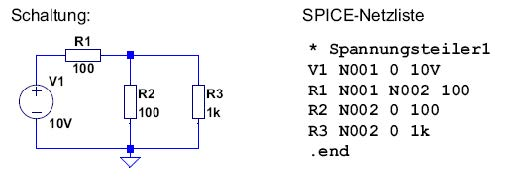
\includegraphics[scale=0.5]{pictures/page1.jpg}
\end{center}

	Eine Netzliste repräsentiert eine Schaltung entsprechend Knoten- und Maschenregel, \newline Viele moderne SPICE Simulationsprogramme
	bieten dem Nutzer jedoch eine grafische Bedienoberfläche. 
	So auch das in diesem Labor verwendete Programm, \textbf{LTSpice XVII}. 


  \end{frame}
  
   \begin{frame}[fragile]{Was ist LTSpice - Installation \& Features}
	
	\begin{enumerate}
\item \href{https://www.analog.com/en/design-center/design-tools-and-calculators/ltspice-simulator.html}{Hier findet Ihr alle Infos vom Hersteller, \textbf{analog devices}}.
\item \href{http://ltspice.analog.com/software/LTspice.dmg}{Installer fuer MacOs http://ltspice.analog.com/software/LTspice.dmg}.
\item \href{http://ltspice.analog.com/software/LTspice.dmg}{Installer fuer MacOs http://ltspice.analog.com/software/LTspice.dmg}.
	\end{enumerate}
	
\begin{center}

\includemedia[
width=0.6\linewidth,height=0.45\linewidth,
addresource=pictures/LTspiceOverview.mp4, %two video files
transparent, %transparent player background
passcontext, %show VPlayer's right-click menu
flashvars={
source=pictures/LTspiceOverview.mp4
}
]{}{VPlayer.swf}

\end{center} 
\end{frame}

 \begin{frame}[fragile]{Ziel dieser Laborübung}

\begin{enumerate}
\item Erarbeiten der Grundlagen zur Simulation mit LTSpice XVII,
\item Eigenständige Simulation von Schaltungen für Studien-/Abschlussarbeiten,
\item Verständnis theoretischer Inhalte mit empirischen Simulationen ergänzen.
\end{enumerate}

\textbf{nächste Schritte}

\begin{itemize}
\item Übungen zum Einstieg in die Simulationswelt,
\item Schrittweise Erarbeitung eines Kleinprojektes \newline \textbf{Simulation einer Temperaturmessbrücke},
\item Simulation digitaler Schaltungen und Bauelemente
\end{itemize}

  \end{frame}
  
\begin{frame}[fragile]{LTSpice XVII - Bitte öffnet alle das Programm}
	
Die Benutzeroberfläche von LTSpice XVII besteht aus den folgenden Elementen.
\begin{spacing}{0.6} \begin{tiny} \textbf{Hinweis:} Die Benutzeroberfläche von LTSpice auf MacOS und Windows unterscheided sich leicht. 
  Die Hautpmenuleiste ist für MacO nicht sichtbar.
  \end{tiny} \end{spacing}

\begin{figure}
  \centering
  \subfloat[Hautpmenuleiste]{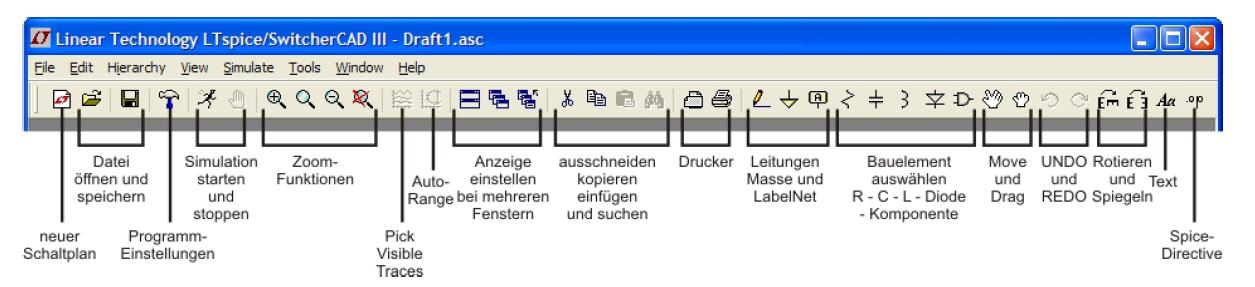
\includegraphics[scale=0.6]{pictures/mainmenu.jpg}}\\
  \subfloat[schematic]{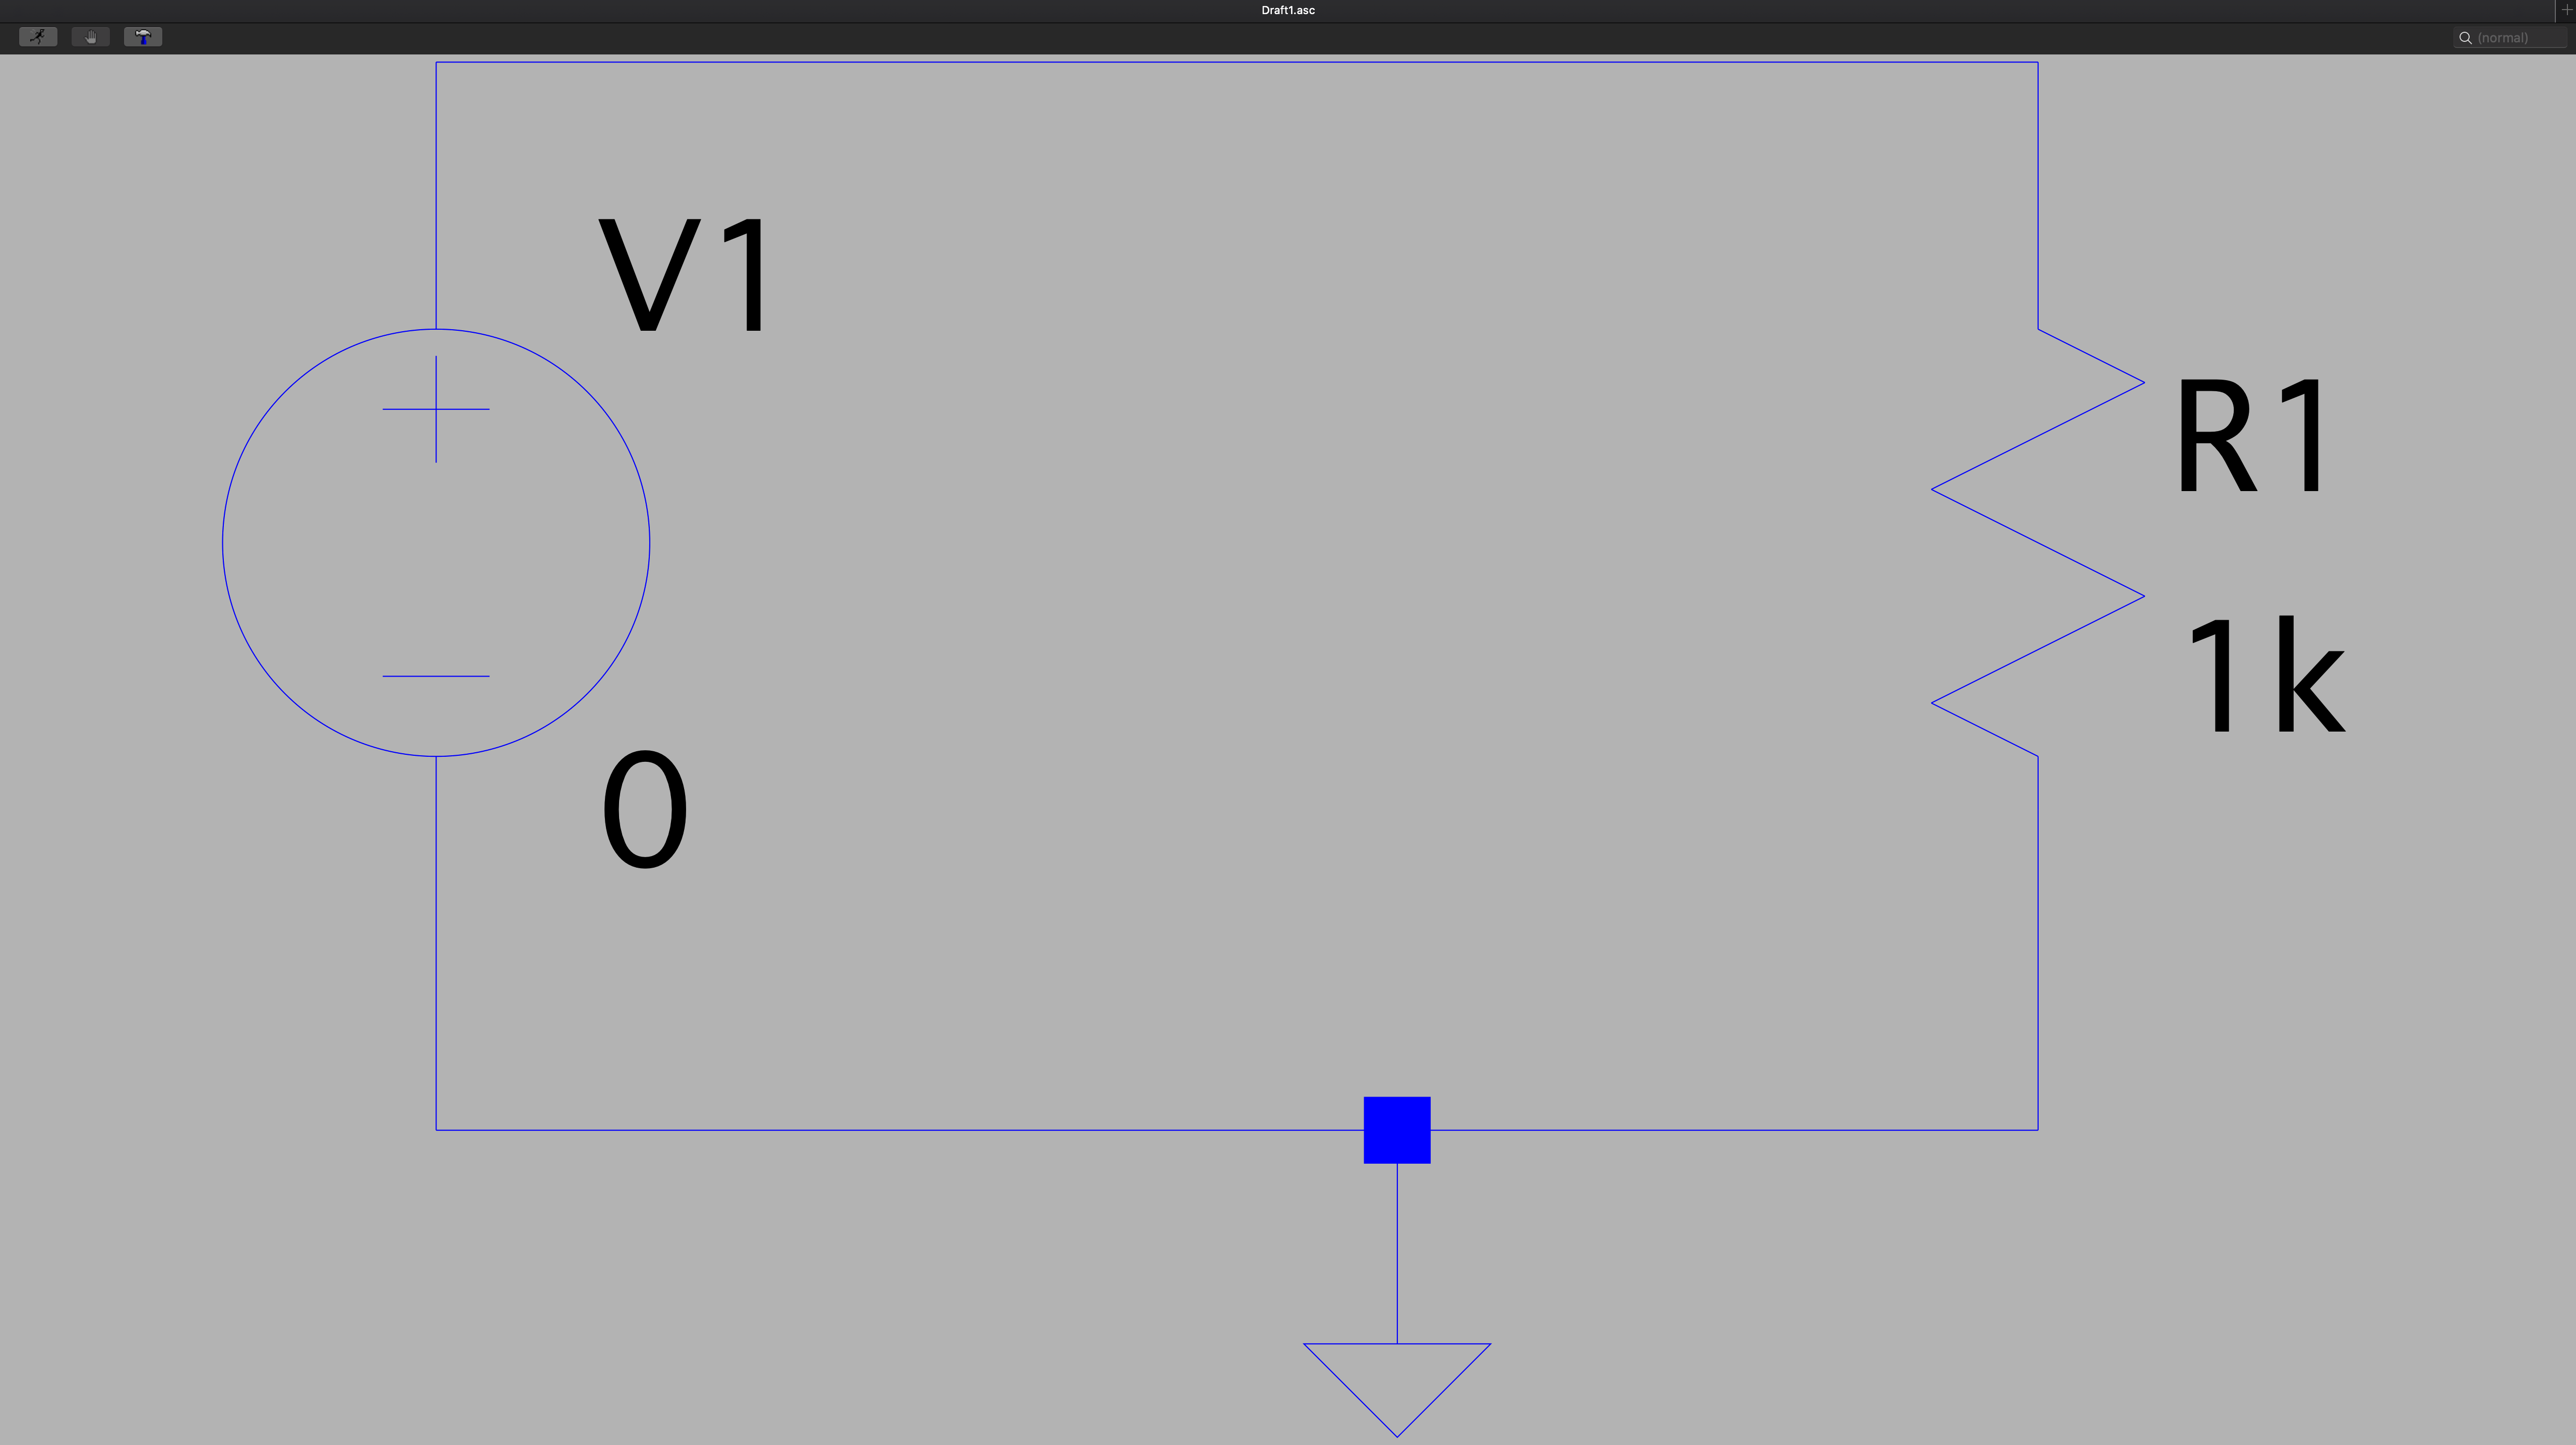
\includegraphics[width=4cm]{pictures/schematic.png}}\qquad    
  \subfloat[waveform]{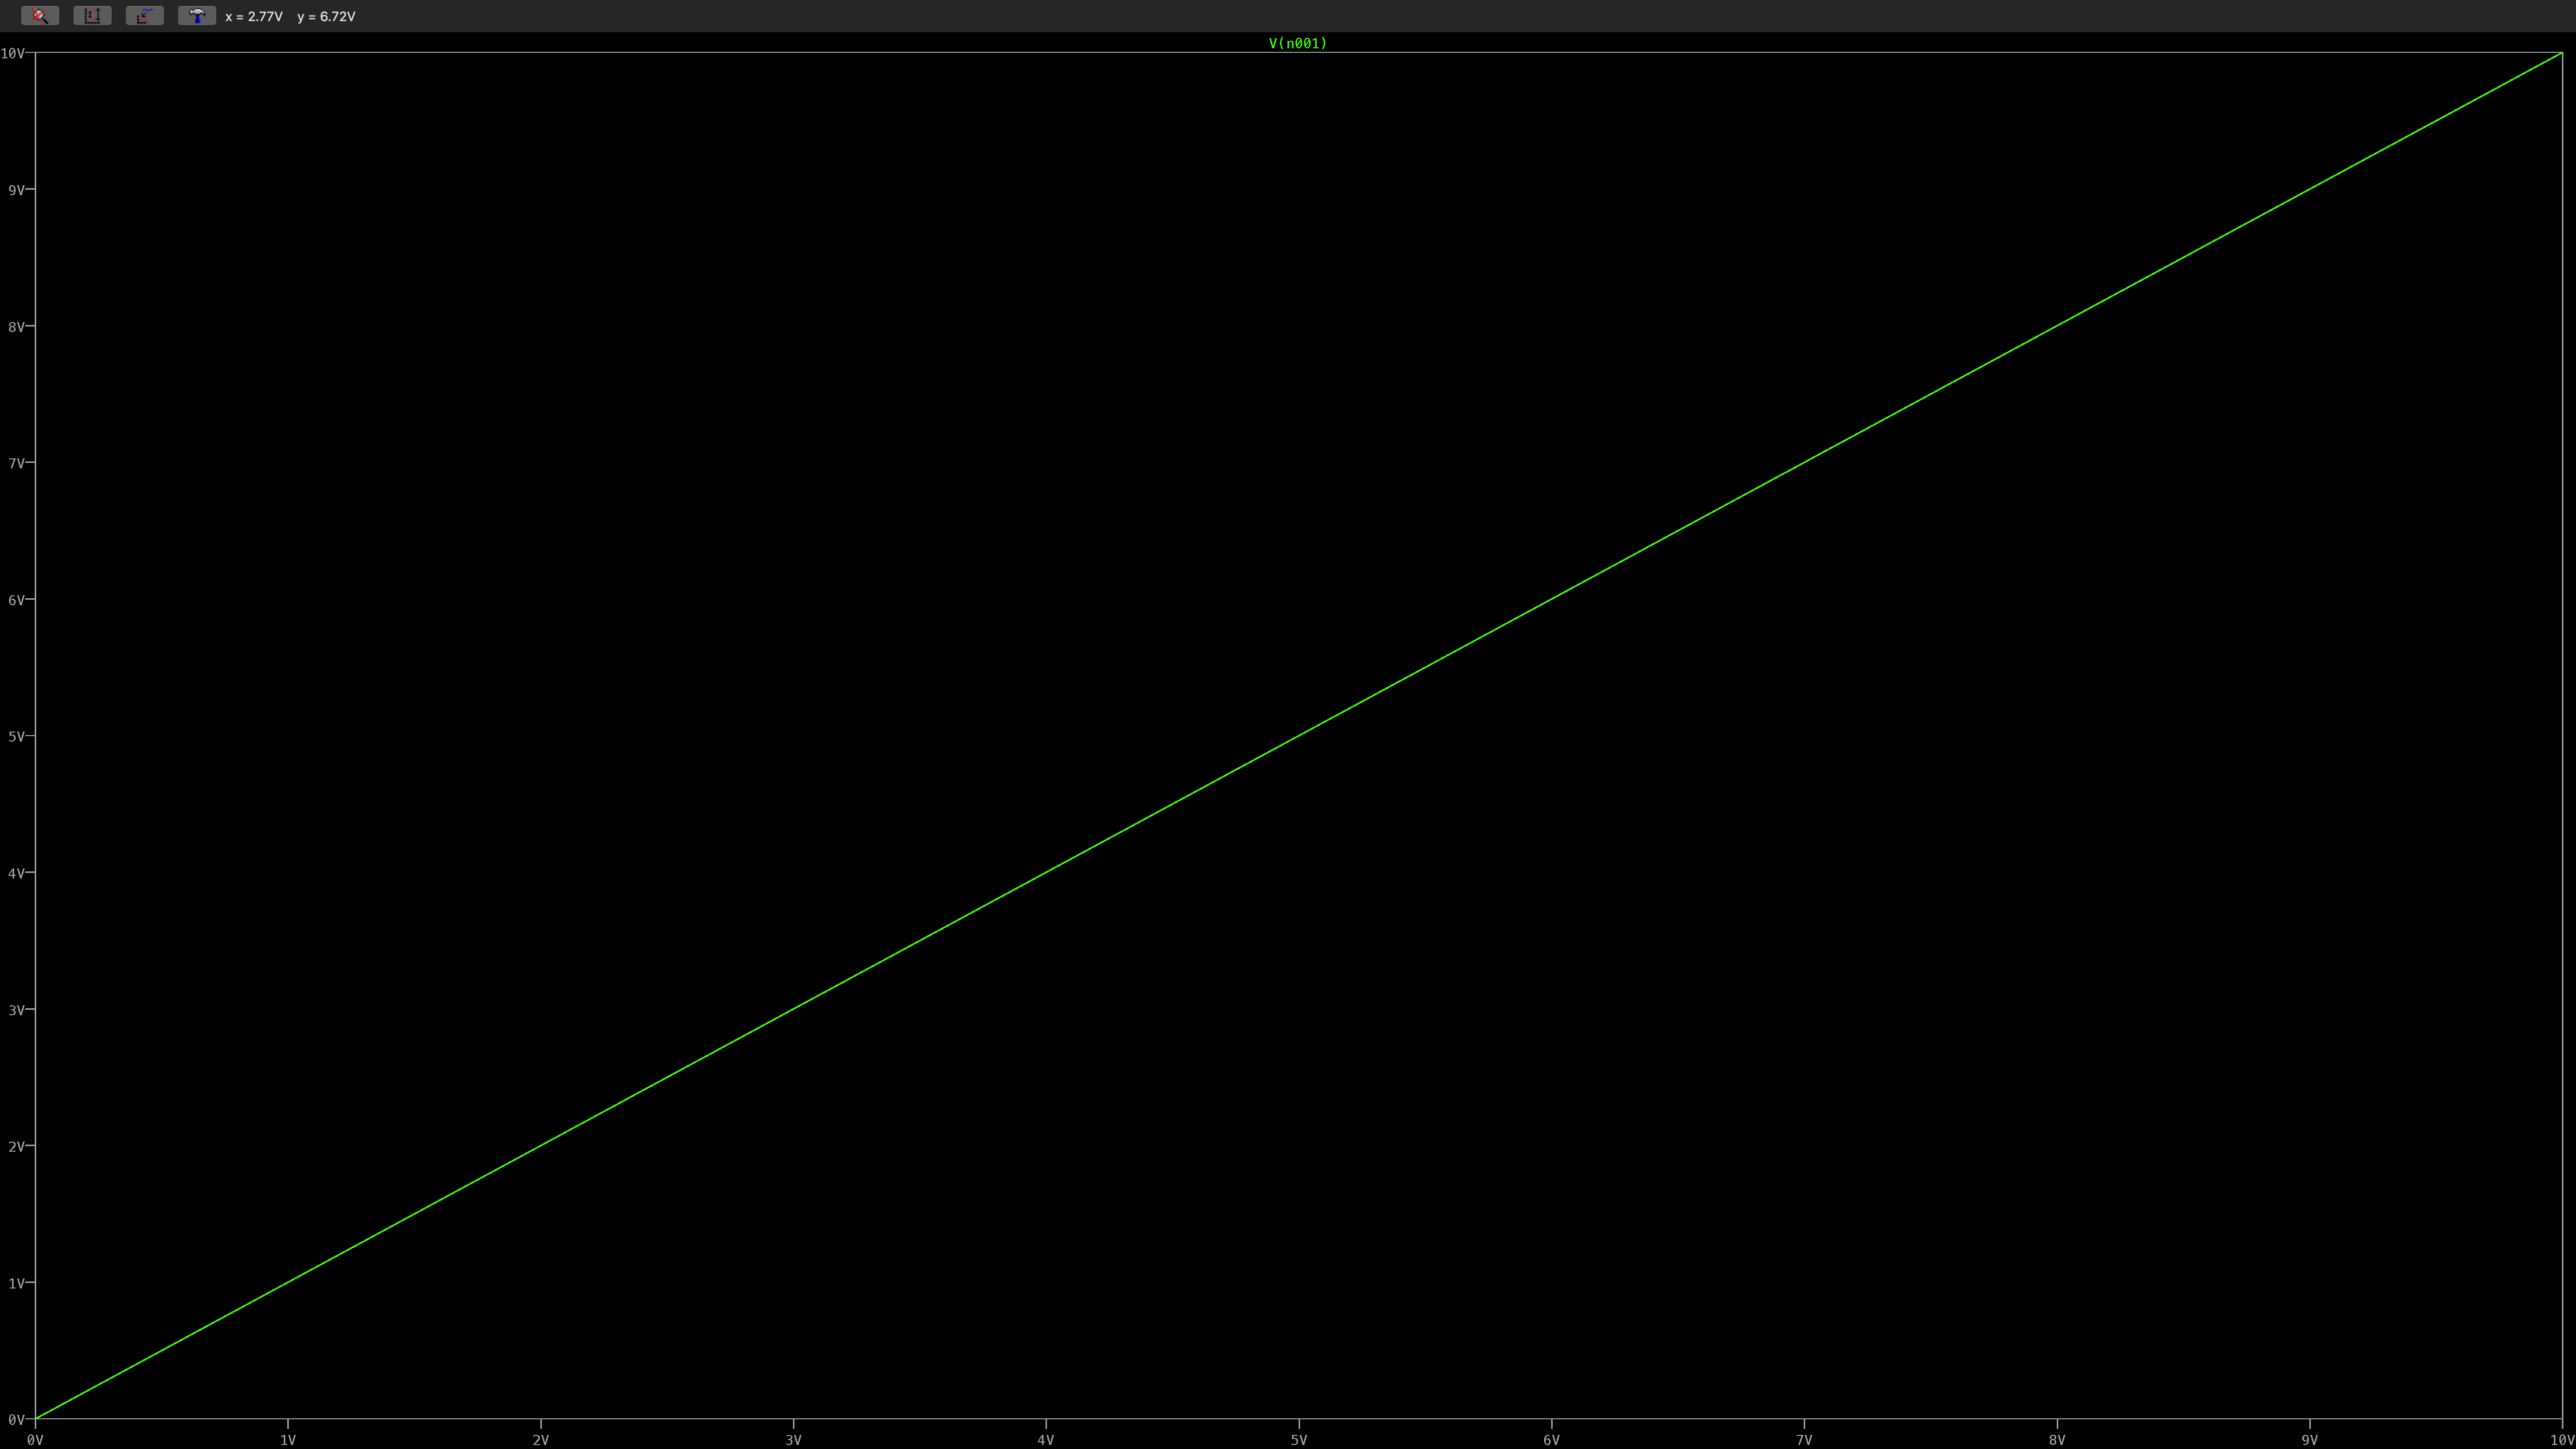
\includegraphics[width=4cm]{pictures/waveform.png}}
\end{figure}

  \end{frame}

  \begin{frame}{LTSpice XVII - Überblick Simulationsarten}

    Die Simulationsart kann im Menu \textbf{Simulation Command} konfiguriert werden. 

    \begin{figure}
      \centering
      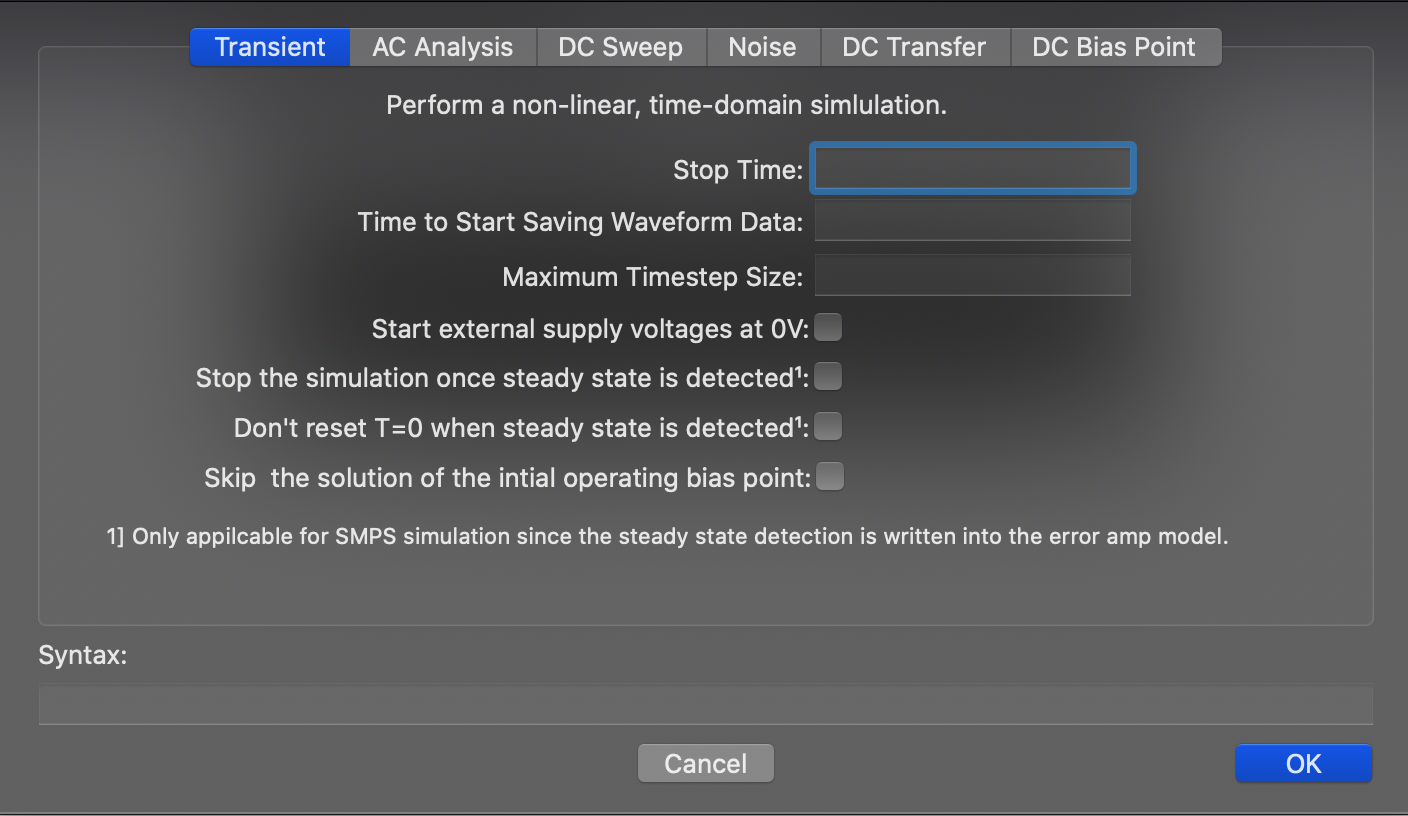
\includegraphics[width=10cm]{pictures/simulationcmd.png}
    \end{figure}
    
  \end{frame}

  \begin{frame}{LTSpice XVII - Überblick Simulationsarten}

    \begin{scriptsize}
    \begin{tabular}{ l }
      \hline
      \textbf{Transient}\\
      Analyse einer Schaltung \textbf{über die Zeit}, z.B. zur Analyse von Einschwingvorgängen\\
      \hline
      \textbf{AC Analysis}\\
      Analyse einer Schaltung \textbf{unter Variantion der Frequenz},\\ z.B. zur Analyse von Grenzfrequenzen\\
      \hline
      \textbf{DC Sweep}\\
      Analyse einer Schaltung \textbf{unter Variation der Spannung},\\ z.B. zur Analyse von Bauteilkennlinien\\
      \hline
      \textbf{Operation Point}\\
      Analyse des \textbf{Arbeitspunktes} einer Schaltung \textbf{ohne Variantion}\\
      \hline
      \textbf{Noise}\\
      Analyse von Rauschverhalten, Bauteilfehlern oder z.B. EMV Einflüssen\\
      \hline
      \textbf{DC Transfer}\\
      Nicht Teil des Labors\\
      \hline
      \textbf{DC Bias Point}\\
      Nicht Teil des Labors\\
      \hline
    \end{tabular}
    \end{scriptsize} 
    
  \end{frame}
  
\begin{frame}[fragile]{Nützliche Voreinstellungen}	

Die Farbdarstellung von LTSpice kann jederzeit konfiguriert werden. Geht dazu über das 
\textbf{control panel} Feld, 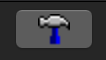
\includegraphics[scale=0.5]{pictures/controlpanel.png} in die Farbeinstellungen
(\textbf{configure colors}). Hier könnt ihr flexibel die Farbdarstellung konfigurieren.

\begin{figure}
  \centering
  \subfloat{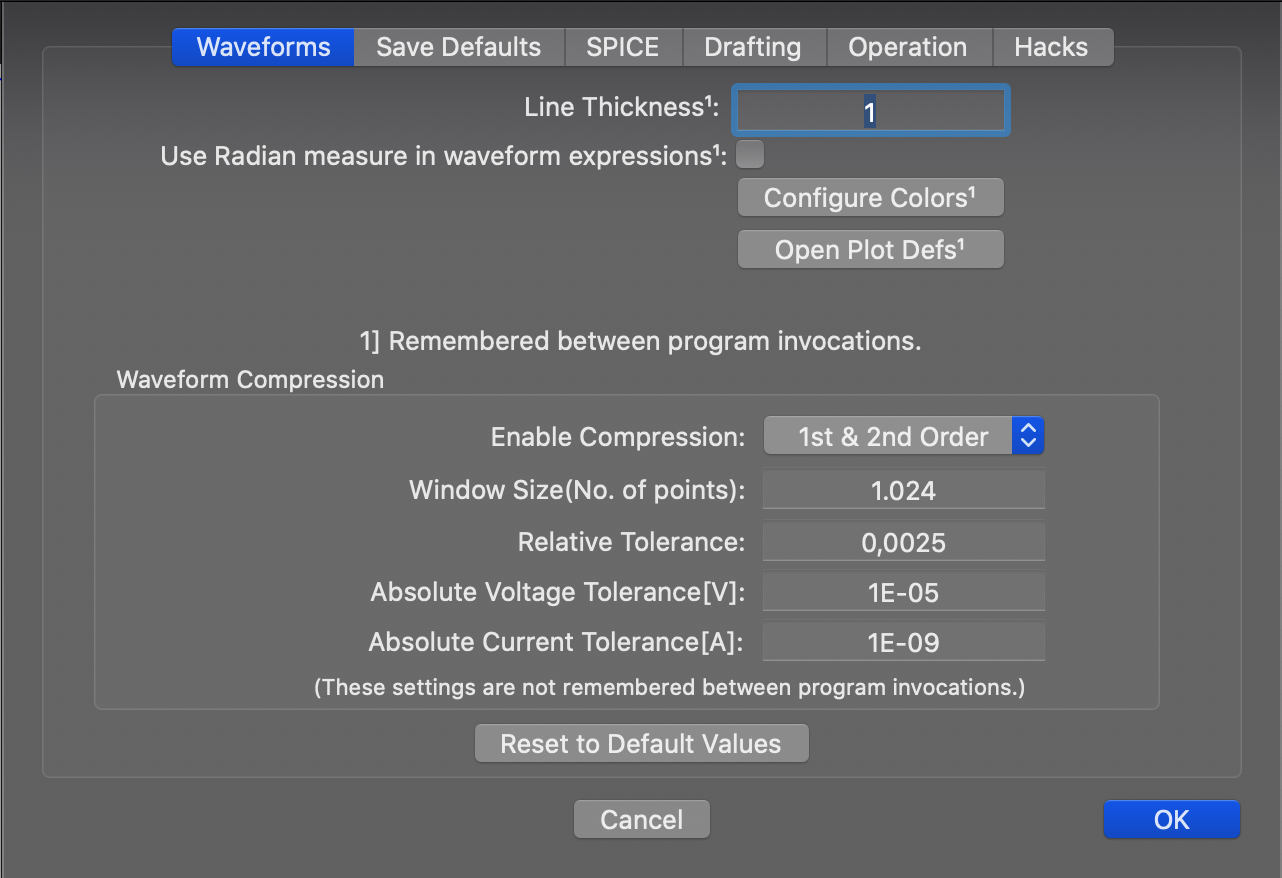
\includegraphics[width=5.5cm]{pictures/controlpanel_2.png}}\qquad    
  \subfloat{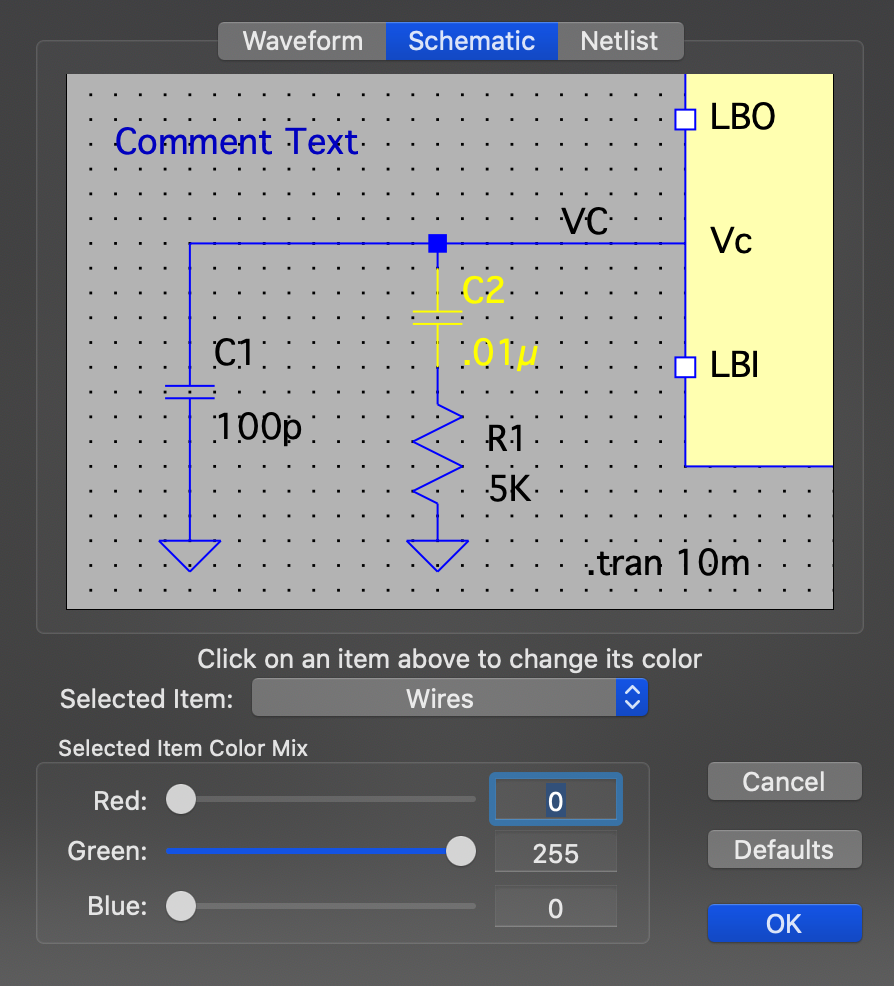
\includegraphics[width=3.5cm]{pictures/colorcfg.png}}
\end{figure}

\end{frame}

\begin{frame}[t]{Shortkeys}
	
Es gibt eine gute Übersicht von HotKeys die die Arbeit mit LTSpice deutlich effektiver macht (nachfolgend sind Hyperlinks embedded).

\begin{itemize}
  \item \href{https://www.analog.com/media/en/simulation-models/spice-models/LTspice_ShortcutFlyer.pdf?modelType=spice-models}{Windows ShortKeys}.
  \item \href{https://www.analog.com/media/en/simulation-models/spice-models/LTspiceShortcutsForMacOSX.pdf?modelType=spice-models}{MacOS ShortKeys}.
  \item \href{https://www.analog.com/media/en/simulation-models/spice-models/LTspiceGettingStartedGuide.pdf?modelType=spice-models}{LTSpice getting started guide}.
\end{itemize}

\begin{figure}
  \centering
  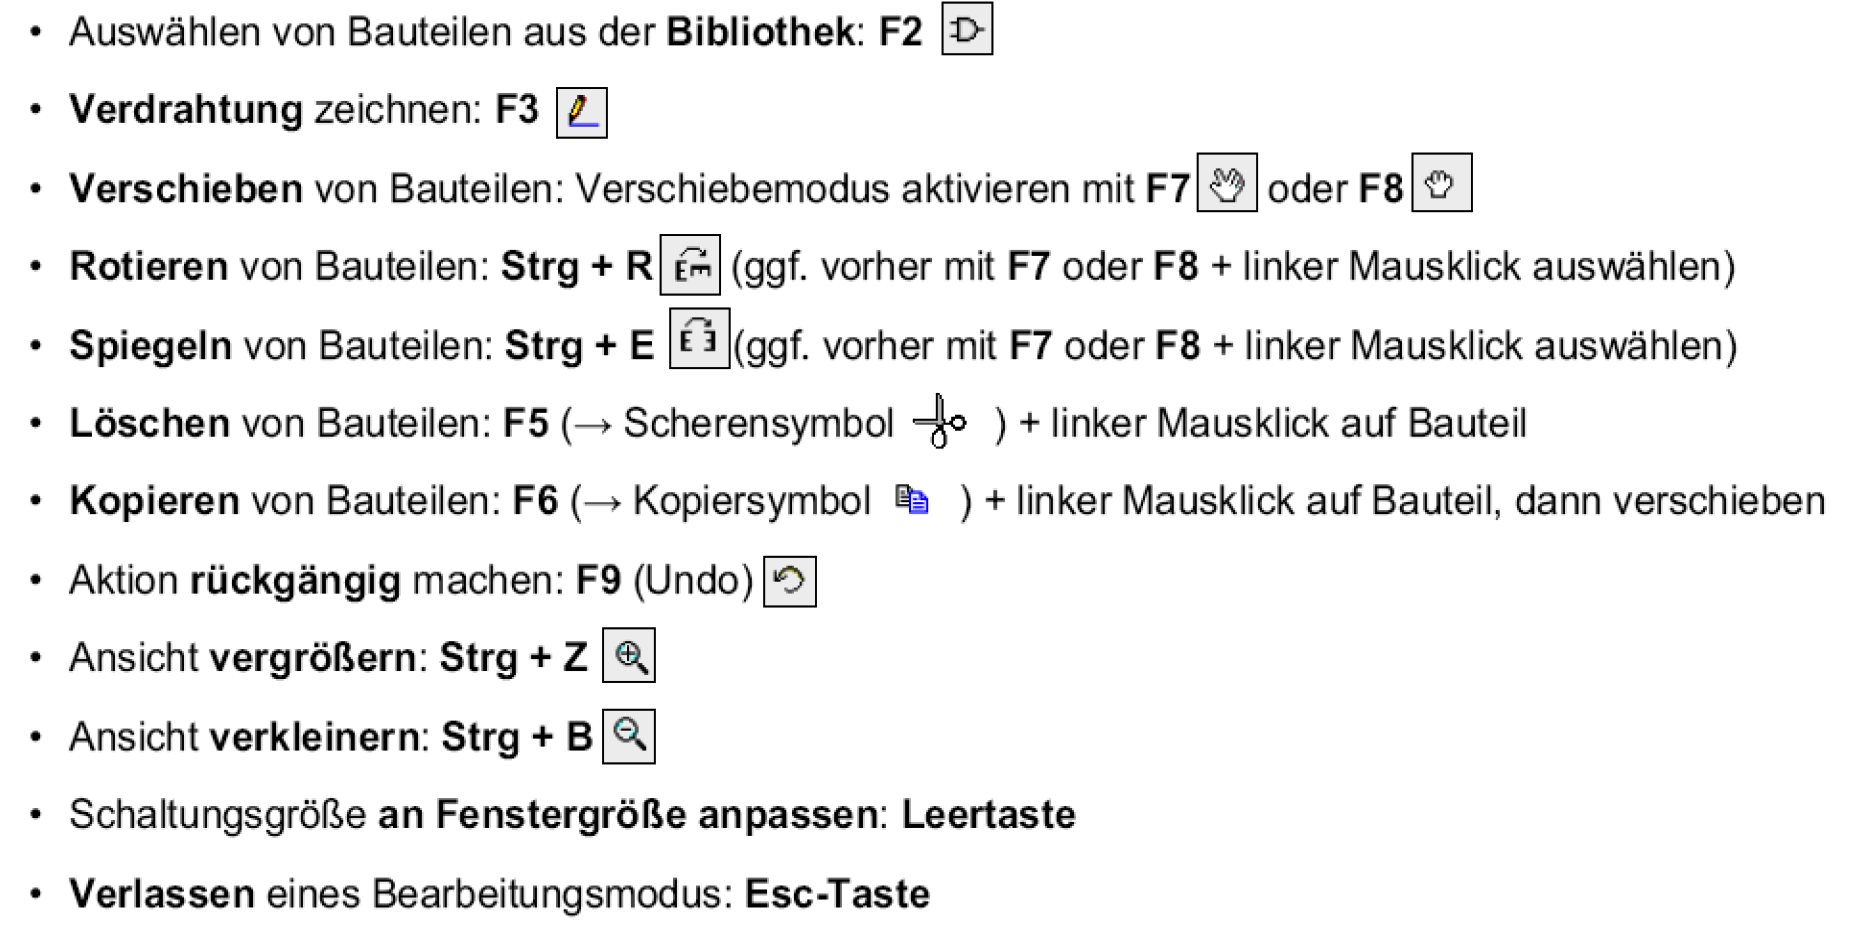
\includegraphics[scale=0.25]{pictures/shortkeys.png}
\end{figure}

\end{frame}

\begin{frame}[t]{Nützliche Hinweise}

  \begin{itemize}
    \item Zahlenwerte immer mit \textbf{Dezimalpunkt statt Komma eingeben! 3.5 anstatt 3,5!}
    \item SPICE arbeitet nach dem Knotenpotenzialverfahren - \textbf{Es muss immer ein Bezugsknoten
          (Masse, Ground) angegeben werden,} sonst treten Simulationsfehler auf (Achtung: Es erfolgt
          keine Fehlermeldung!).
  \end{itemize}

\end{frame}
  
\section{Hands-on LTSpice - Das Labor beginnt}
  
  
\begin{frame}[fragile]{Vorgehensweise}

  Diese Übungen sind zur interaktiven Arbeit mit LTSpice gedacht. 
  Sie führen von der Aufgabe über den Lösungsansatz bis hin zur fertigen Analyse.
  
  Bitte geht nach den folgenden Schritten vor, um die Übungen strukturiert zu bearbeiten. 
  
  \begin{enumerate}
\item \textbf{Schematic modellieren}
\item \textbf{Simulationsart analysieren}
\item \textbf{Simulationsart konfigurieren}
\item \textbf{Ergebnis mit der Vorgabe abgleichen}
\end{enumerate}

Sollte es zu Problemen kommen, bitten wir euch uns direkt einen Hinweis zu geben!

  \end{frame}
  
  \section{Übungen}
  
\begin{frame}[t]{ohmscher Widerstand}

    \textbf{Ziel - Darstellung von Bauteilkennlinie}
    
    \begin{spacing}{0.6} \begin{tiny}
    
    Das ohmsche Gesetz $U=R I$ lässt sich mit Hilfe eines kleinen Schaltungsexperimentes gut visualisieren und nachvollziehen. 
    Hierzu werden wir die folgende Schaltung aufbauen und den Stromverlauf über dem Widerstand darstellen. 
    \end{tiny} \end{spacing}
    \begin{spacing}{0.9} \begin{tiny}
    \begin{table}[h!]
      \begin{tabular}{p{3cm} p{7cm}}
        \hline
        \textbf{Erstellung des Schaltplans} & \\
        \hline \\
        \begin{minipage}{.3\textwidth}
          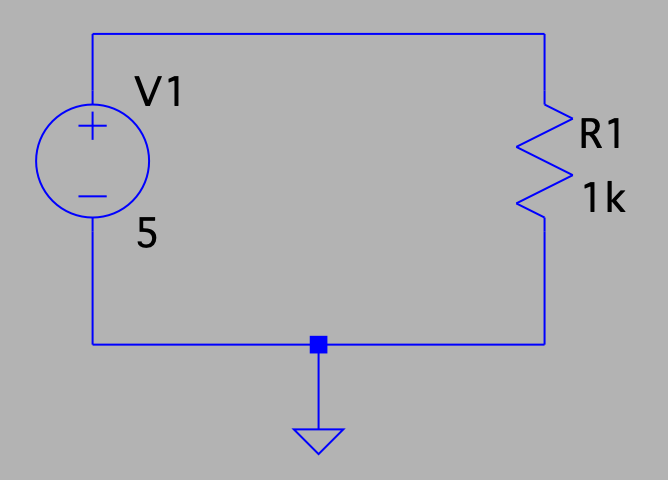
\includegraphics[width=\linewidth]{pictures/res.png}
        \end{minipage} 
        & 
        \begin{minipage}{.7\textwidth}
        \begin{itemize}
          \item Erstellt ein neues schematic (File $->$ new schematic)
          \item Speichert es direkt als neue Dateil ab (File $->$ save as)
          \item Öffnet den Bauteileditor (\textbf{F2}) und für eine Spannungsquelle hinzu (voltage)
          \item Öffnet erneut den Bauteileditor und für einen Widerstand hinzu (resistor bzw. EuropeanResistor fuer die bekannte Box-Darstellung)
          \item Fügt einen Masseknoten als Bezugsknoten hinzu (\textbf{F4}).
          \item Verdrahtet die Schaltung (\textbf{F3})
        \end{itemize}
        \end{minipage} 
        \\
         & \\
         \hline
         \textbf{Konfiguration der Simulation} & \\
         \hline \\
         \begin{minipage}{.3\textwidth}
          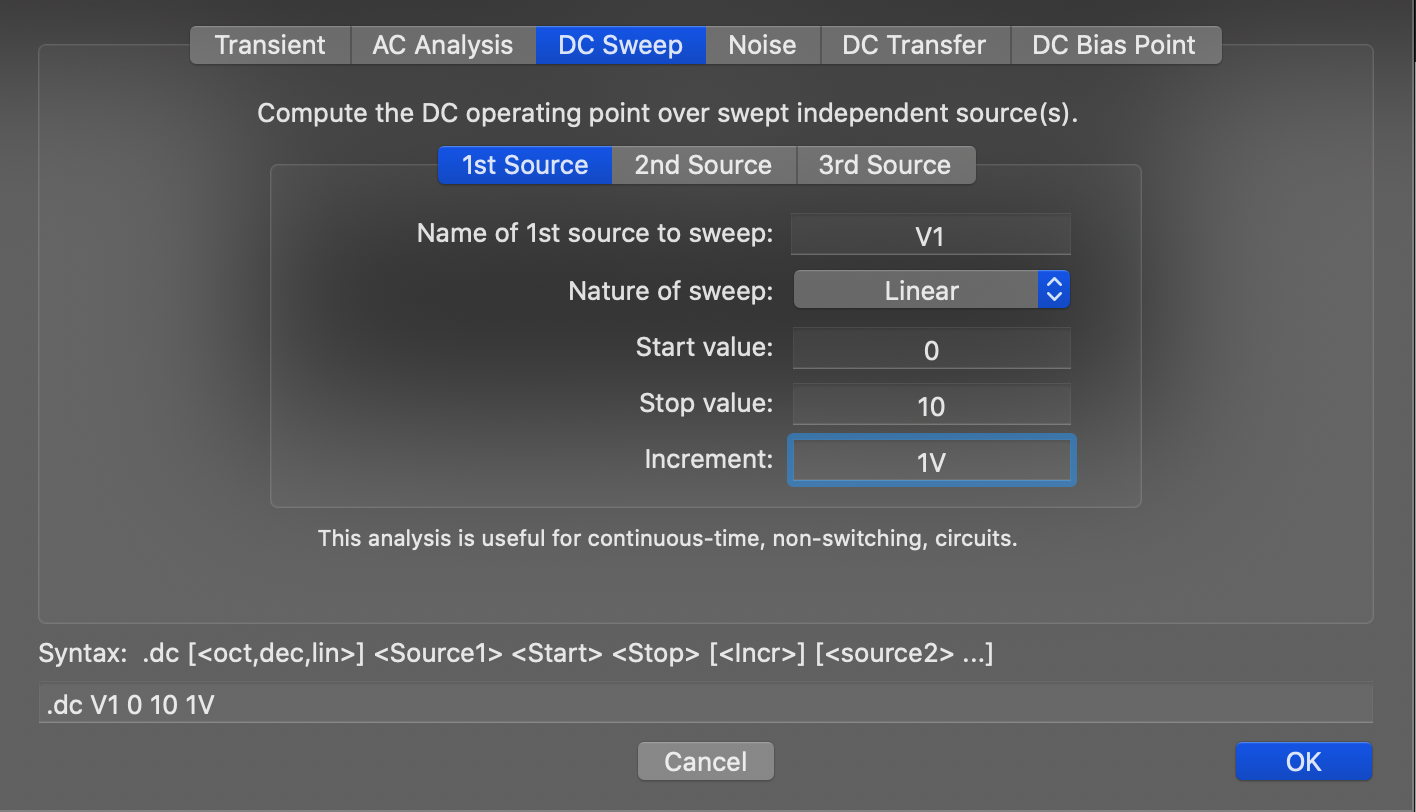
\includegraphics[width=\linewidth]{pictures/simulationcmd_1.png}
        \end{minipage} 
        & 
        \begin{minipage}{.7\textwidth}
        \begin{itemize}
          \item Im Menu Simulation, wählt \textbf{Edit simulation command} und wählt den DC Sweep. 
          \item Unser Ziel ist es den Stromverlauf über dem Widerstand zu simulieren
          \item Daher konfigurieren wir die Spannungsquelle \textbf{V1} mit einem \textbf{linearen} Sweep von 0 bis 10 V mit einer \textbf{Schrittweite} von 1V.
          \item Bestätigt mit \textit{OK} und fügt die Sumlationsansweisung dem schematic hinzu
        \end{itemize}
        \end{minipage} 
        \\
         & \\
         \hline
      \end{tabular}
    
    \end{table}
    
    \end{tiny} \end{spacing}
    
     \end{frame}
    
     \begin{frame}[t]{ohmscher Widerstand}
    
      \begin{spacing}{0.9} \begin{tiny}
      \begin{table}[h!]
        \begin{tabular}{p{5cm} p{5cm}}
          \hline
          \textbf{Simulation und Analyse} & \\
          \hline \\
          \begin{minipage}{.5\textwidth}
            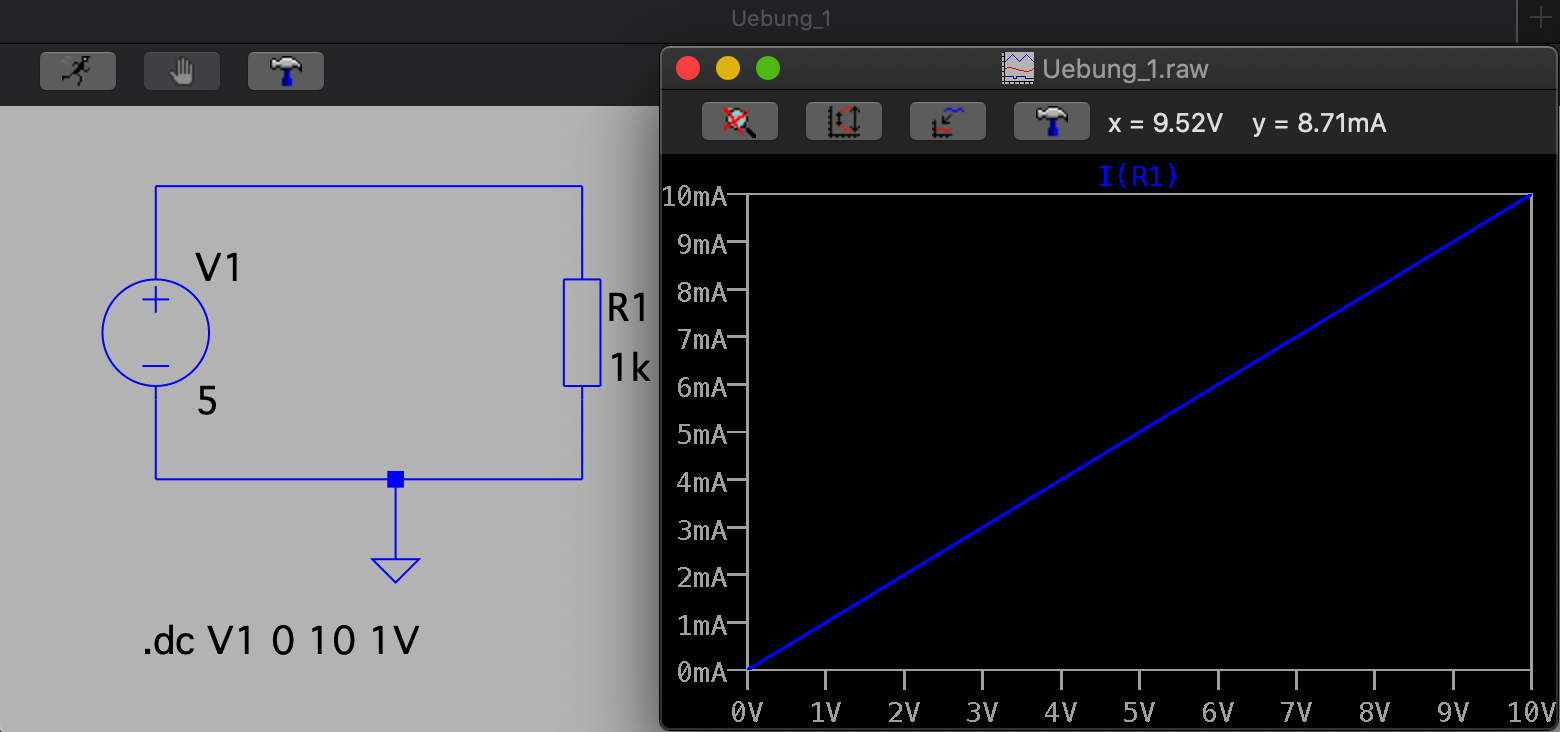
\includegraphics[width=\linewidth]{pictures/analysis.png}
          \end{minipage} 
          & 
          \begin{minipage}{.5\textwidth}
          \begin{itemize}
            \item Klickt auf 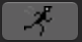
\includegraphics[scale=0.3]{pictures/run.png} (run) und LTspice startet die Simulation
            \item Der waveform viewer öffnet sich - ihr könnt auf zwei Arten Strom, Spannung und Leistungen aus eurer Schaltung anzeigen lassen. \newline\newline
            \textbf{Im schematic} könnt ihr über ein Bauteil mit der Maus fahren und es erscheint eine Stromzange\newline\newline
            \textbf{Im schematic} könnt ihr über ein Bauteil mit der Maus fahren, Shift gedrückt halten und es erscheint eine Leistungsmessanzeige\newline\newline
            \textbf{Im schematic} könnt ihr über eine Knoten mit der Maus fahren und es erscheint ein Spannungsmesser\newline\newline
            \textbf{Im waveform viewer} könnt ihr über rechten Mausklick $->$ add trace die verfügbaren Messtellen direkt auswählen
            \item Wir wählen \textbf{I(R1)}, den Strom durch unseren Widerstand R1. 
          \end{itemize}
          \end{minipage} 
          \\
        \end{tabular}
      \end{table}
    \end{tiny} \end{spacing}
    
      \begin{spacing}{0.9} \begin{tiny}
        \begin{table}[h!]
          \begin{tabular}{p{10cm} }
            \hline
            \textbf{Ergebnis und Auswertung} \\
            \hline \\    
            Wie zu erwarten liefert dieses einfache Beispiel den Zusammenhang zwischen Strom, Spannung und Widerstand. Probiert an dieser Stelle gerne die Spannung, Schrittweite
            zu variieren oder weitere Werte im waveform viewer anzueigen zu lassen.
          \end{tabular}
        \end{table}
      \end{tiny} \end{spacing}
      
       \end{frame}%resistor
\begin{frame}[t]{Diode}

    \textbf{Ziel - Darstellung von Bauteilkennlinie}
    
    \begin{spacing}{0.6} \begin{tiny}
    
    Eine Diode wird oft durch Ihre Durchlassspannung klassifiziert. Dies ist die Spannung ab der die Diode leitend wird. Leitend ist Sie, wenn ein Strom fließt. Dieses Verhalten möchten
    wir in einem kleinen simulativen Experiment herausarbeiten. 
    \end{tiny} \end{spacing}
    \begin{spacing}{0.9} \begin{tiny}
    \begin{table}[h!]
      \begin{tabular}{p{3cm} p{7cm}}
        \hline
        \textbf{Erstellung des Schaltplans} & \\
        \hline \\
        \begin{minipage}{.3\textwidth}
          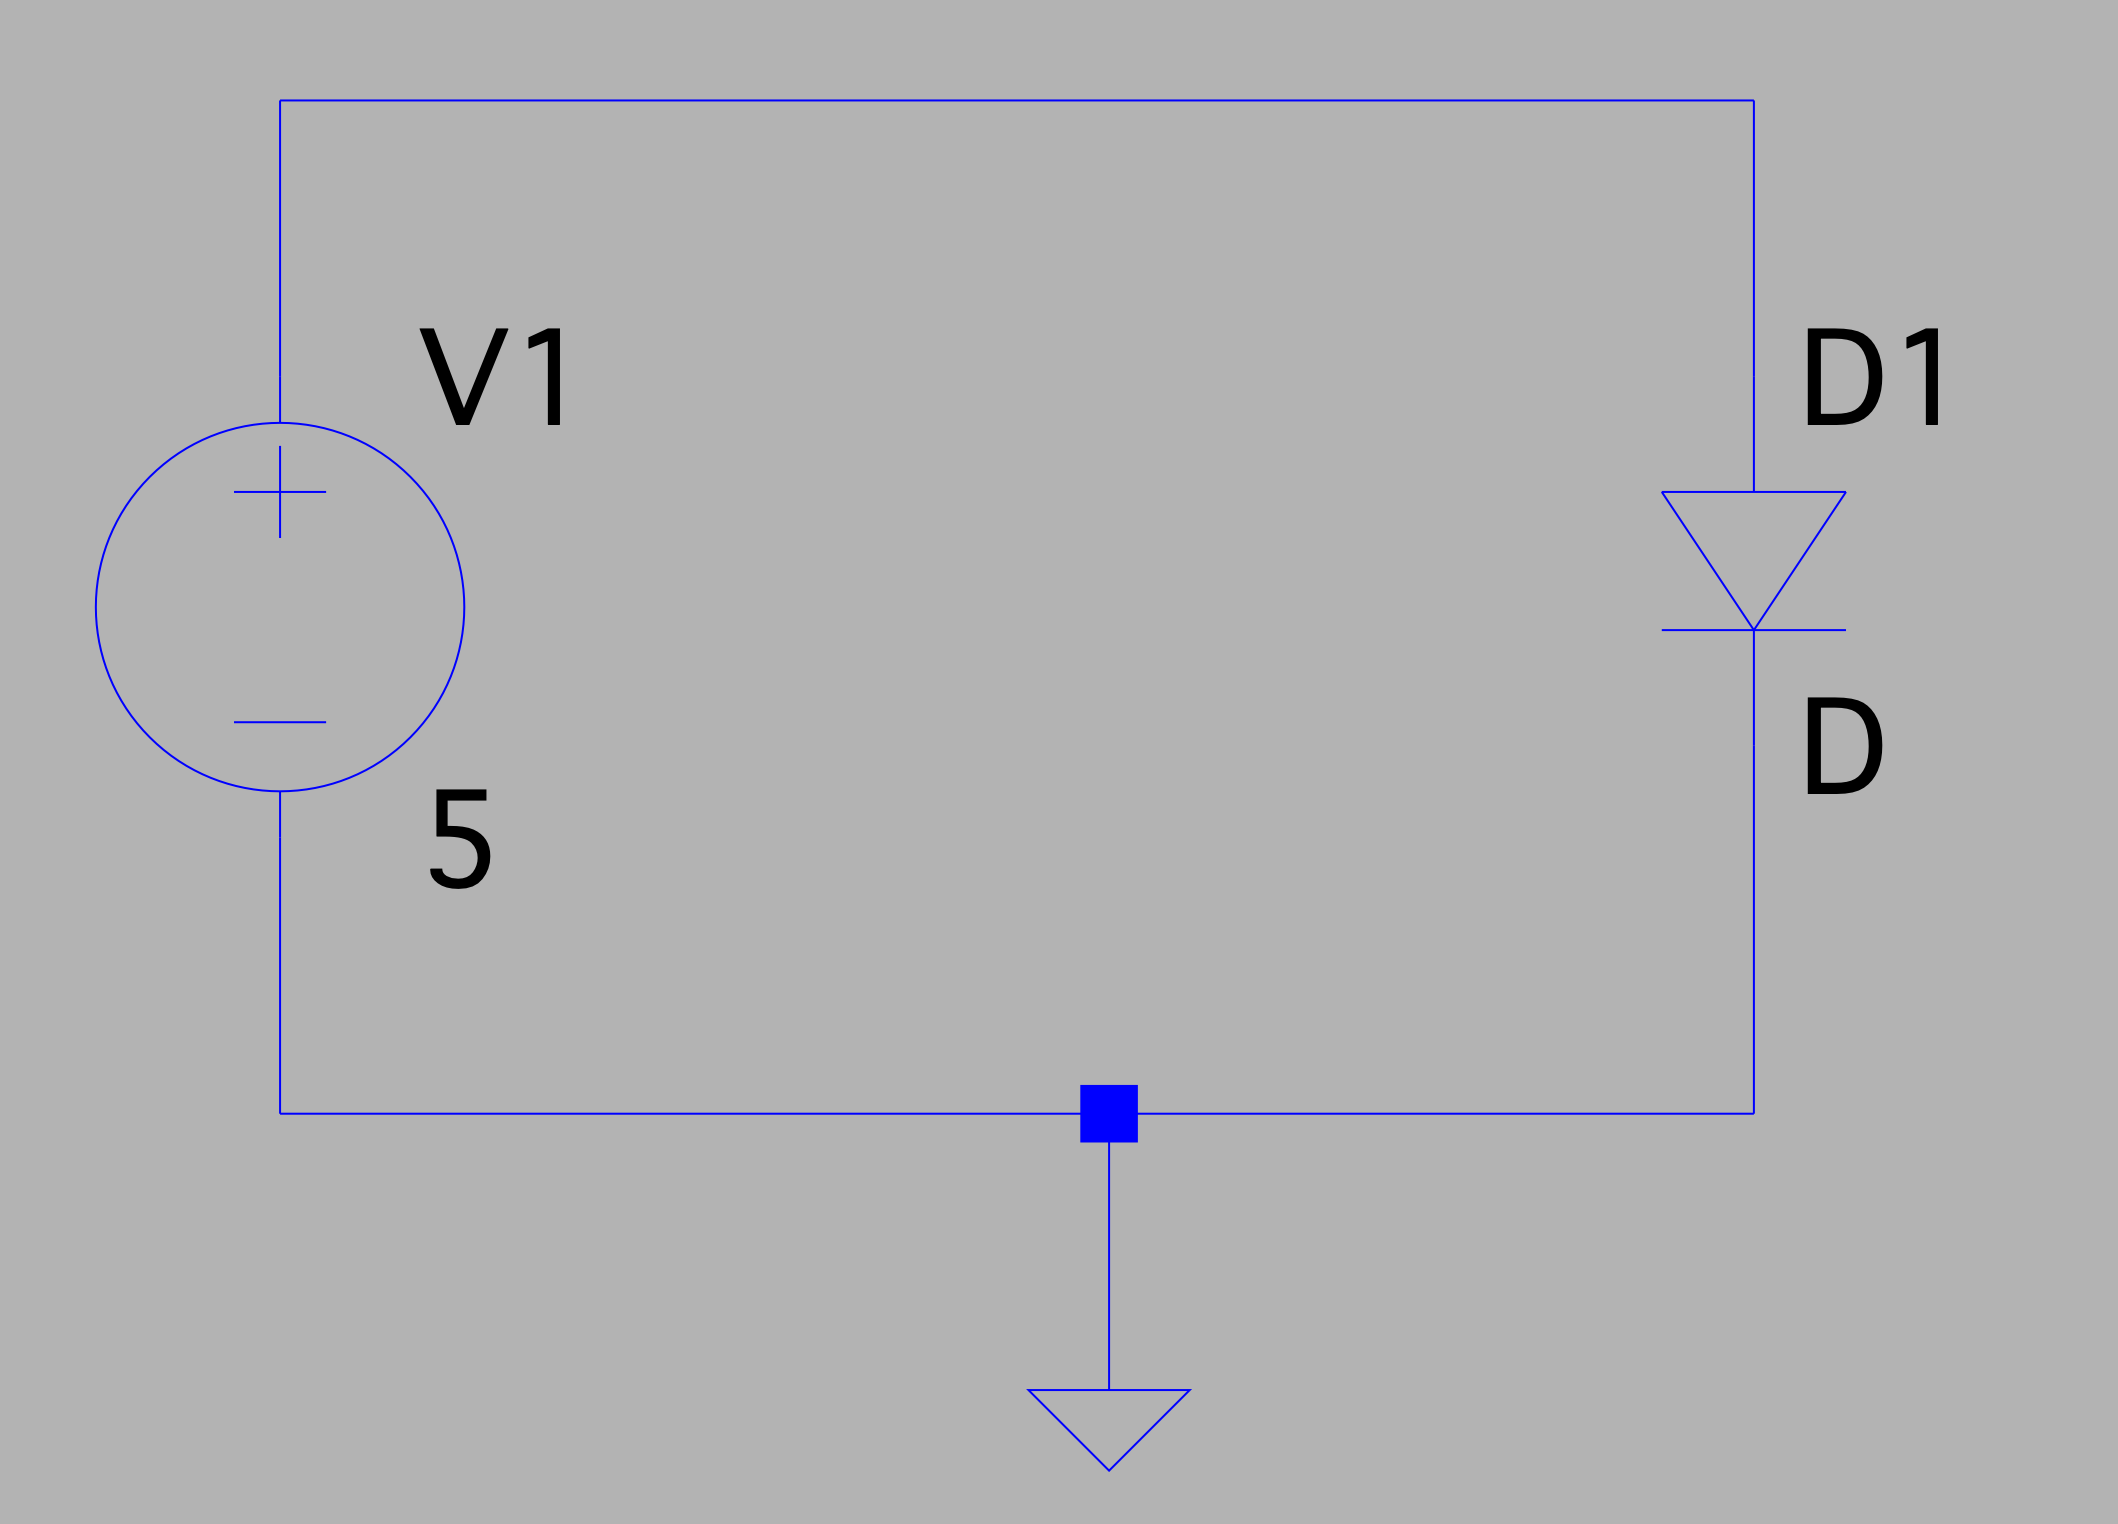
\includegraphics[width=\linewidth]{pictures/diode.png}
        \end{minipage} 
        & 
        \begin{minipage}{.7\textwidth}
        \begin{itemize}
          \item Speichert das Projekt direkt als neue Datei ab (File $->$ save as ) 
          \item Löscht den Wiederstand heraus (\textbf{F5}) 
          \item Öffnet erneut den Bauteileditor (\textbf{F2}) und für eine einfache Diode hinzu (sucht nach Diode \dots)
          \item Verdrahtet die Schaltung wieder vollstänndig (\textbf{F3})
        \end{itemize}
        \end{minipage} 
        \\
         & \\
         \hline
         \textbf{Konfiguration der Simulation} & \\
         \hline \\
         \begin{minipage}{.3\textwidth}
          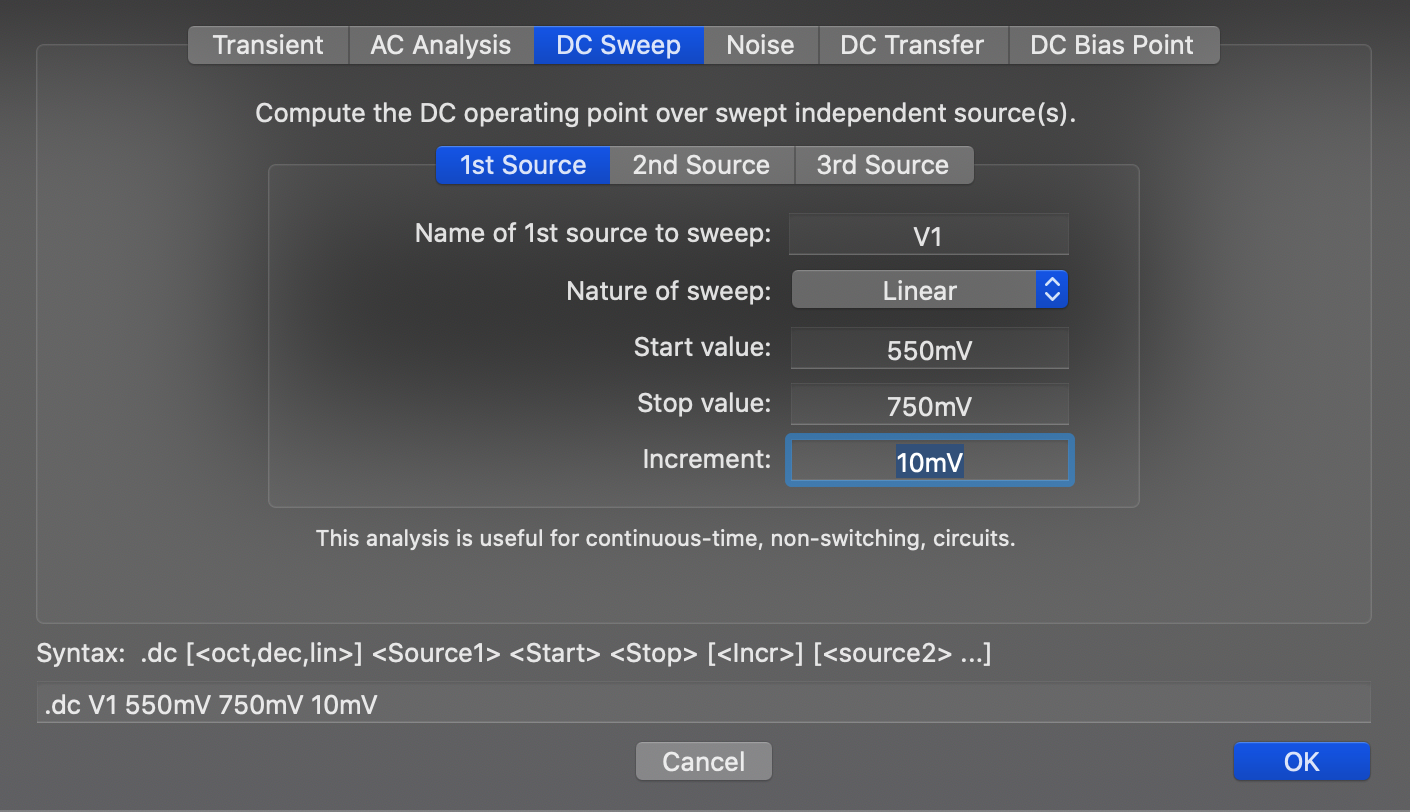
\includegraphics[width=\linewidth]{pictures/simulationcmd_2.png}
        \end{minipage} 
        & 
        \begin{minipage}{.7\textwidth}
        \begin{itemize}
          \item Im Menu Simulation, wählt \textbf{Edit simulation command} und bliebt beim DC Sweep. 
          \item Unser Ziel ist es den Stromverlauf durch die Diode zu messen. Dafür müssen wir die Spannung erhöhen. 
          Wir wissen, dass die notwendige Spannung im Bereich 600 - 700 mV liegen muss. 
          \item Daher konfigurieren wir die Spannungsquelle \textbf{V1} mit einem \textbf{linearen} Sweep von 550 bis 750 mV mit einer \textbf{Schrittweite} von 10 mV.
          \item Bestätigt mit \textit{OK} und fügt die Sumlationsansweisung dem schematic hinzu
        \end{itemize}
        \end{minipage} 
        \\
         & \\
         \hline
      \end{tabular}
    
    \end{table}
    
    \end{tiny} \end{spacing}
    
     \end{frame}
    
     \begin{frame}[t]{Diode}
    
      \begin{spacing}{0.9} \begin{tiny}
      \begin{table}[h!]
        \begin{tabular}{p{5cm} p{5cm}}
          \hline
          \textbf{Simulation und Analyse} & \\
          \hline \\
          \begin{minipage}{.5\textwidth}
            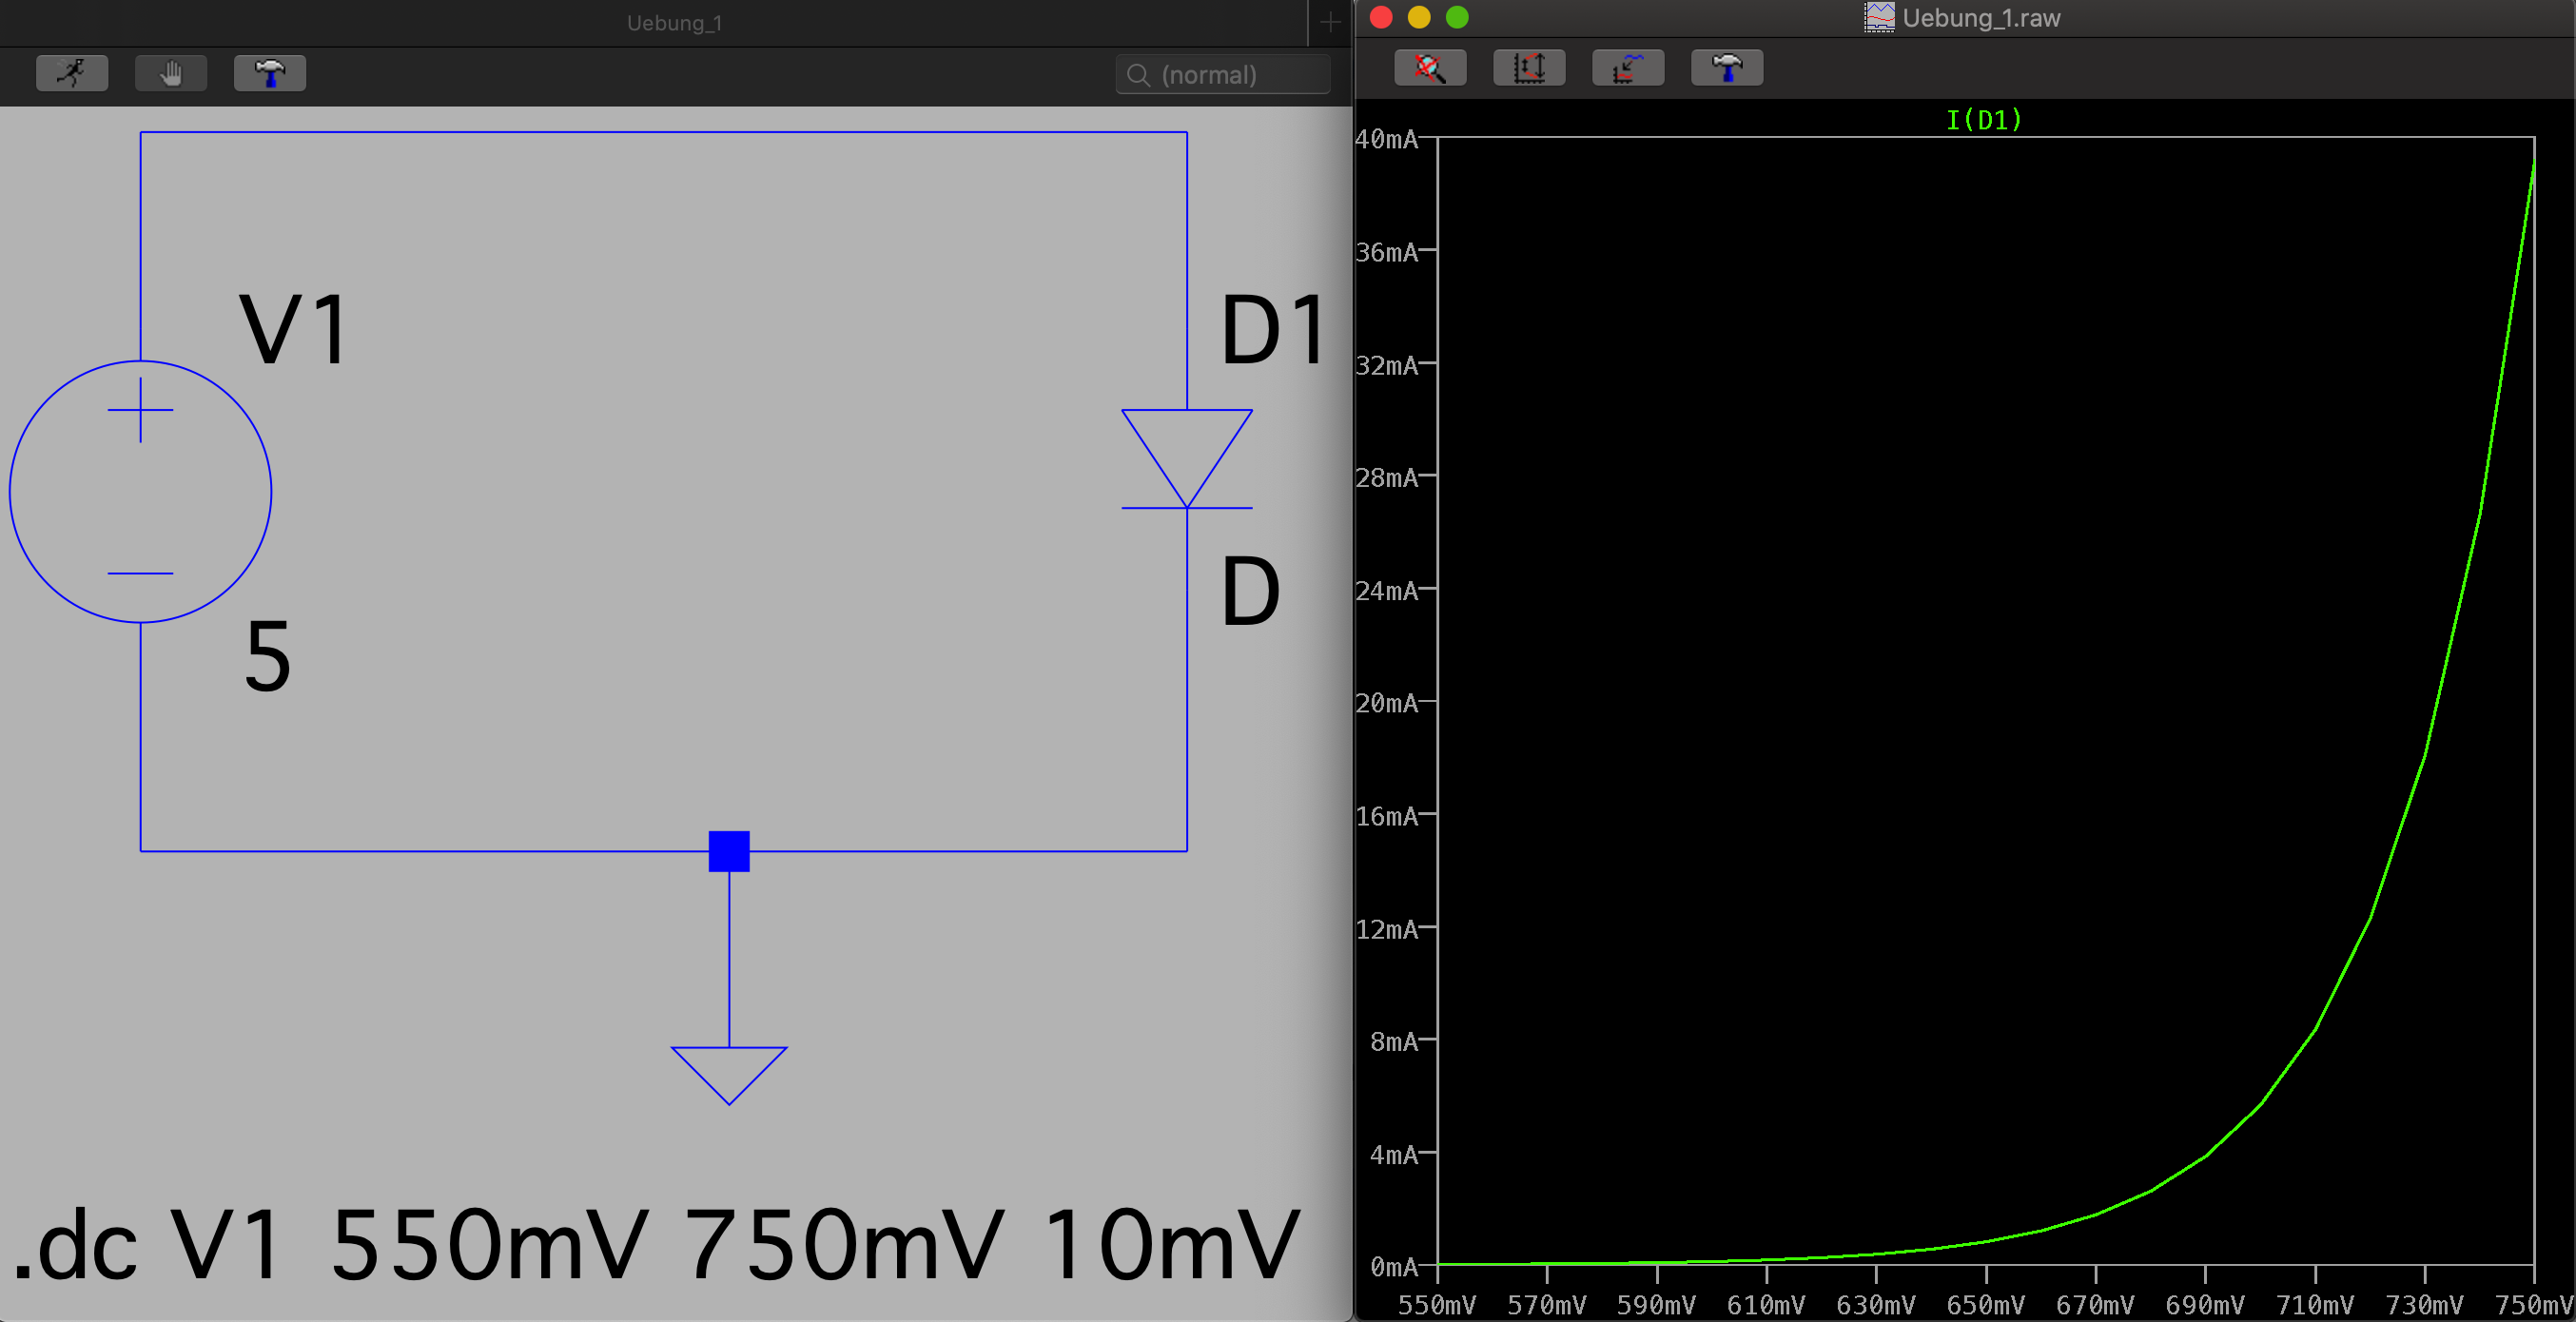
\includegraphics[width=\linewidth]{pictures/analysis_2.png}
          \end{minipage} 
          & 
          \begin{minipage}{.5\textwidth}
          \begin{itemize}
            \item Klickt auf 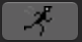
\includegraphics[scale=0.3]{pictures/run.png} (run) und LTSpice startet die Simulation
          \item Wir wählen \textbf{I(D1)}, den Strom durch die Diode.
          \end{itemize}
          \end{minipage} 
          \\
        \end{tabular}
      \end{table}
    \end{tiny} \end{spacing}
    
      \begin{spacing}{0.9} \begin{tiny}
        \begin{table}[h!]
          \begin{tabular}{p{10cm} }
            \hline
            \textbf{Ergebnis und Auswertung} \\
            \hline \\    
            Wie zu erwarten liefert dieses einfache Beispiel den Zusammenhang zwischen Strom, Spannung und Wiederstand. Probiert den Spannungsbereich des
            DC-Sweep von 550 - 750 mV auf 550 mV - 2V zu erhöhen.          
            \begin{itemize}
              \item Was fällt euch auf?
              \item Könnt ihr euch herleiten, warum man eine 
              Diode immer mit einem Vorwiederstand betreiben sollte? 
            \end{itemize}  
            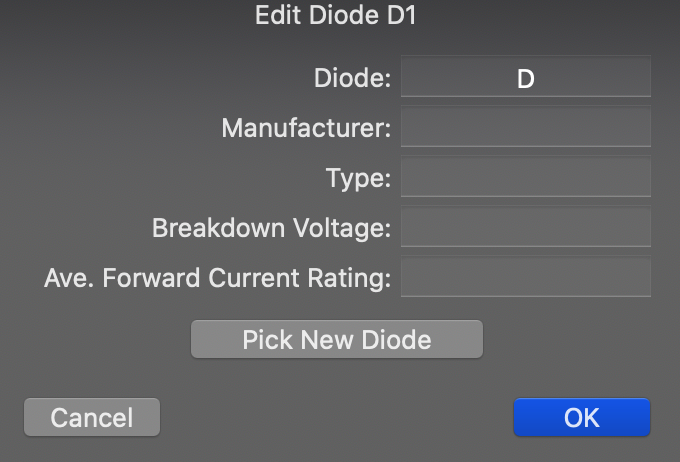
\includegraphics[scale=0.1]{pictures/diode_choice.png} \newline
            Mit einem rechten Mausklick auf die Diode könnte ihr die Dioden Typen variieren. (\textbf{pick new diode})
            Zum Beispiel von einer idealen aus dem obigen Beispiel zu einer beliebigen realen entsprechend dem Modell des Herstellers, schaut euch die Unterschiede an.
          \end{tabular}
        \end{table}
      \end{tiny} \end{spacing}
      
       \end{frame}%diode
\begin{frame}[t]{NPN-Transistor}

  \textbf{Ziel - Darstellung des Ausgangskennlinienfeld}

  \begin{spacing}{0.6} \begin{tiny}

      Das Ausgangskennlinienfeld eines npn Transistors beschreibt den Zusammenhang von Kollektorstrom $I_c$ und der Spannung
      an der Kollektor-Emitter Strecke $U_{ce}$. Das Kennlinienfeld wird für verschiedene Basisströme $I_b$ angegeben.
    \end{tiny} \end{spacing}
  \begin{spacing}{0.9} \begin{tiny}
      \begin{table}[h!]
        \begin{tabular}{p{3cm} p{7cm}}
          \hline
          \textbf{Erstellung des Schaltplans}   & \\
          \hline                                  \\
          \begin{minipage}{.3\textwidth}
            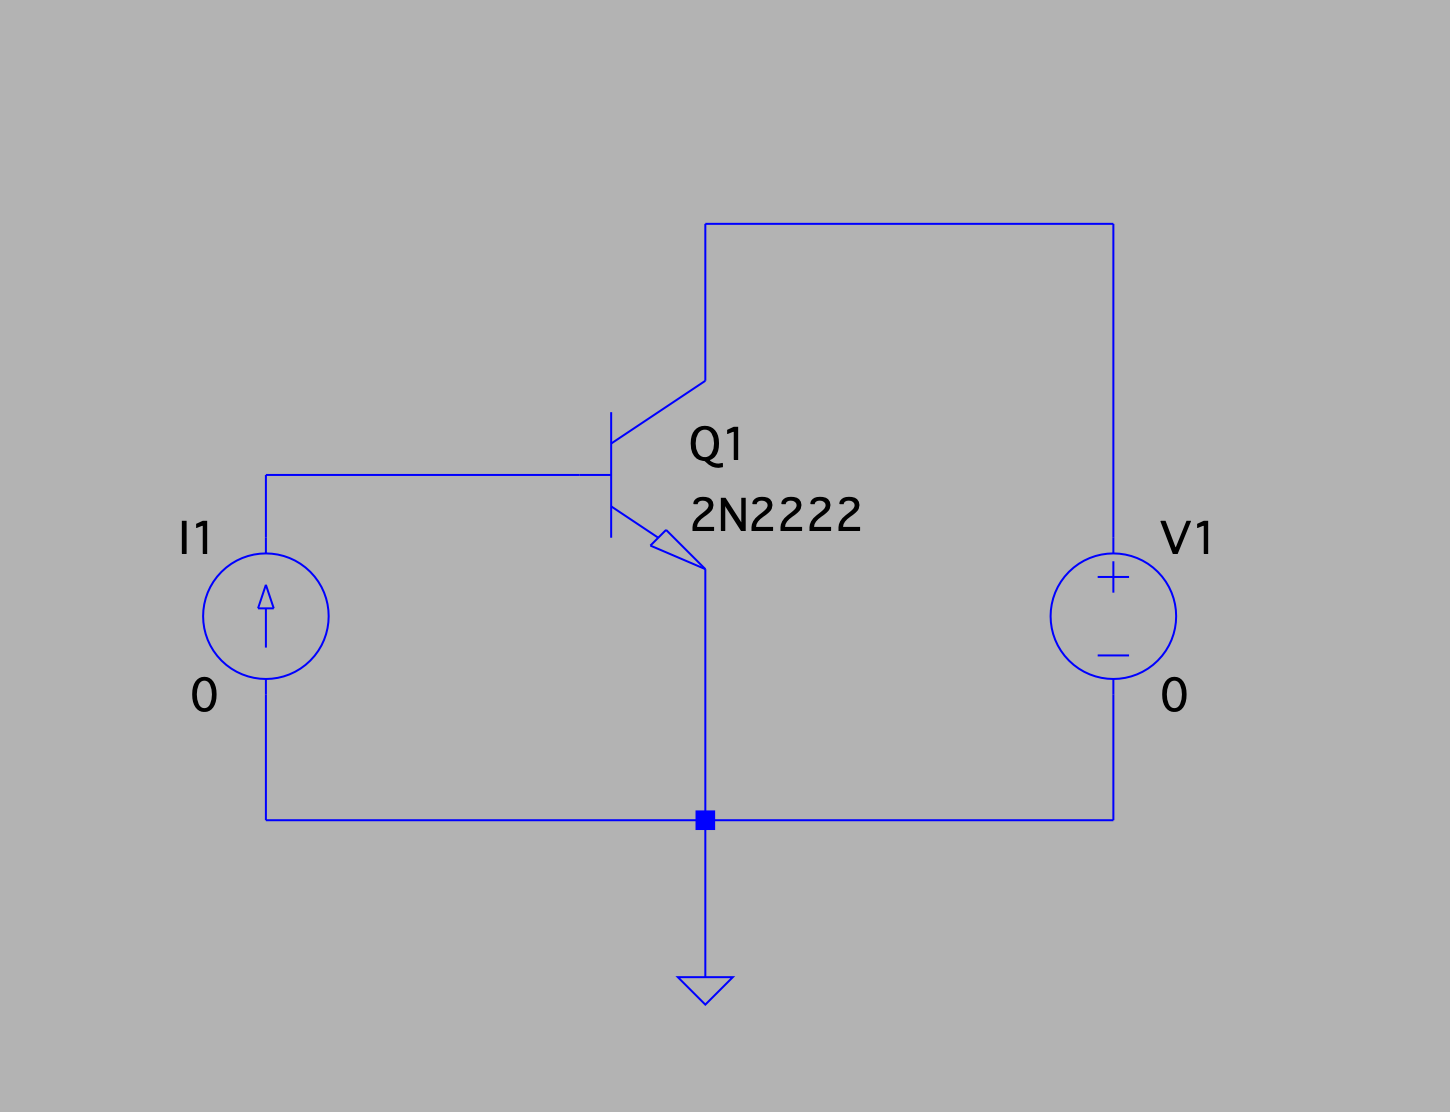
\includegraphics[width=\linewidth]{pictures/tran.png}
          \end{minipage}
                                                &
          \begin{minipage}{.7\textwidth}
            \begin{itemize}
              \item Startet mit einem neuen schematic
              \item Speichert das Projekt direkt als neue Datei ab (File $->$ save as )
              \item Fügt eine ideale Stromquelle (\textbf{F2} \dots current) hinzu und dreht dieser (\textbf{STRG+R})
              \item Fügt einen npn-Transistor(\textbf{F2} \dots npn) hinzu.
              \item Per rechtem Mausklick könnt ihr vom idealen npn anlaog zur Diode im letzten Beispiel zum 2N2222 wechseln.
              \item Verdrahtet die Schaltung wieder vollstänndig (\textbf{F3})
            \end{itemize}
          \end{minipage}
          \\
                                                & \\
          \hline
          \textbf{Konfiguration der Simulation} & \\
          \hline                                  \\
          \begin{minipage}{.3\textwidth}
            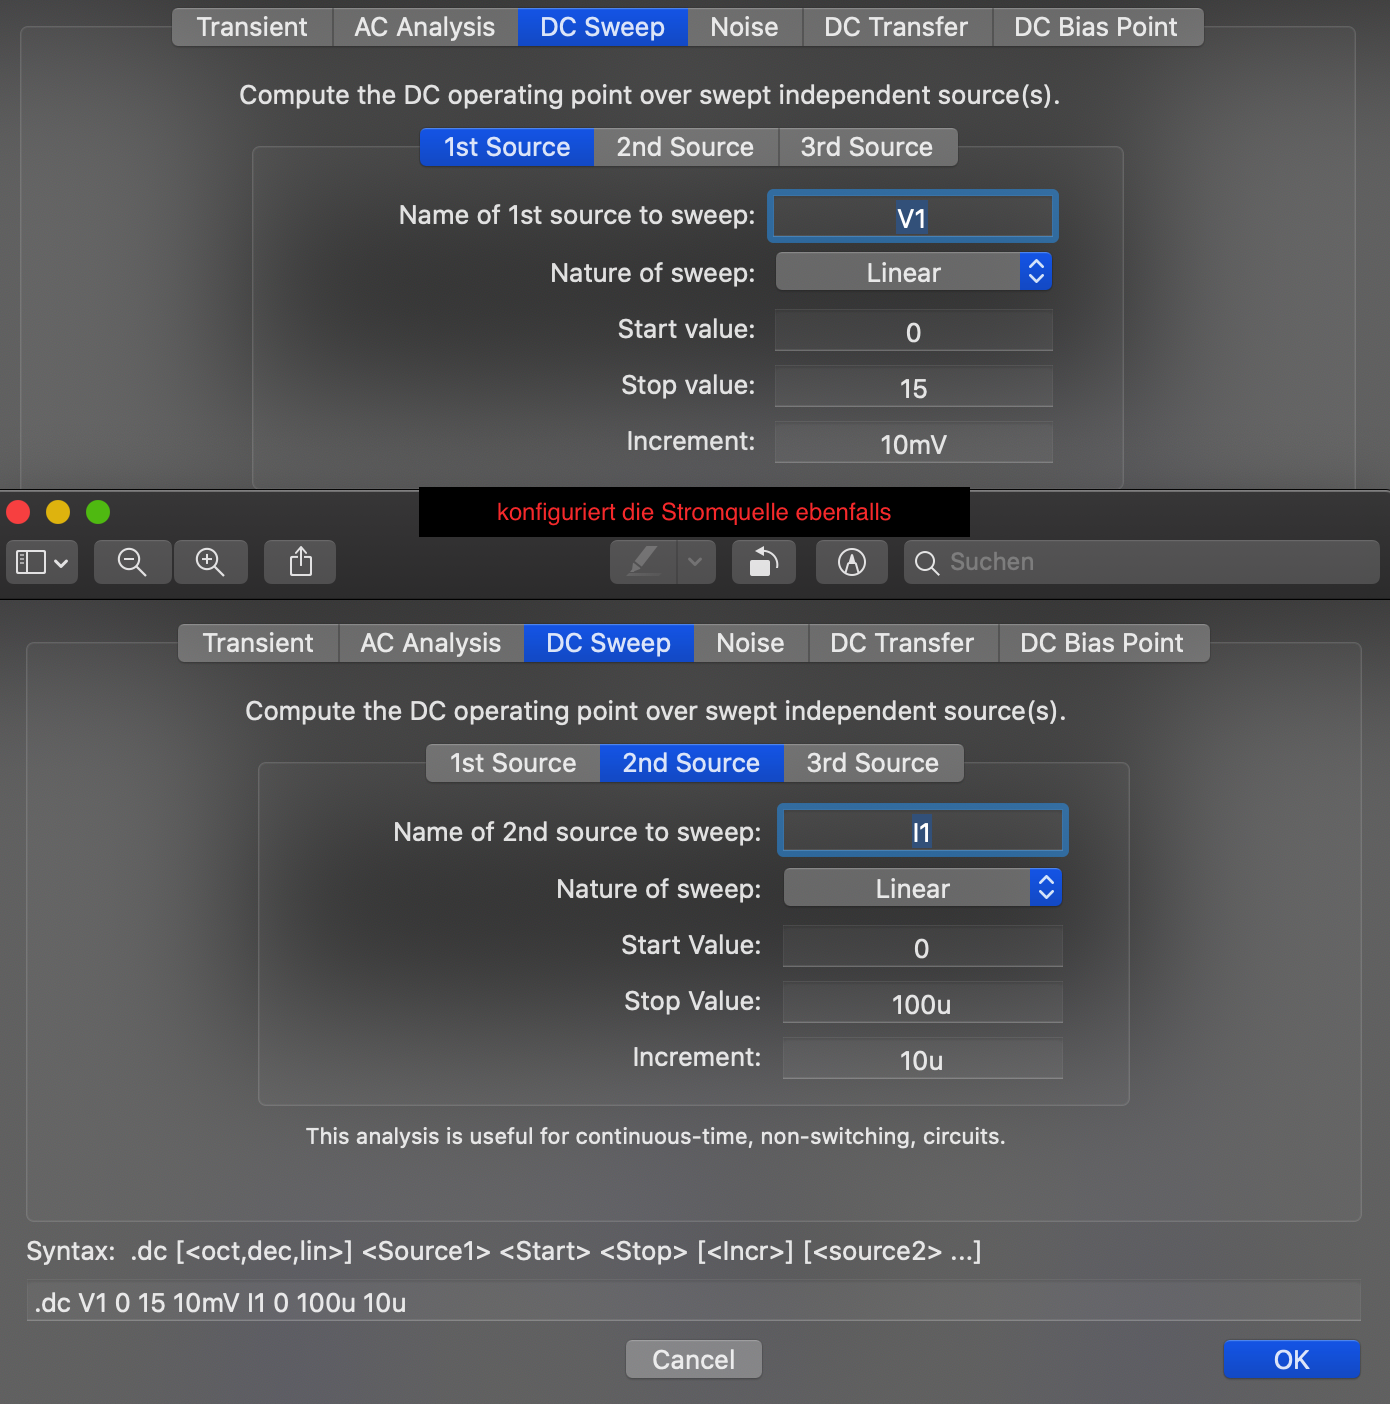
\includegraphics[width=0.8\linewidth]{pictures/simulationcmd_3.png}
          \end{minipage}
                                                &
          \begin{minipage}{.7\textwidth}
            \begin{itemize}
              \item Im Menu Simulation, wählt \textbf{Edit simulation command} und bliebt beim DC Sweep.
              \item Unser Ziel ist es das Ausgangskennlinienfeld des 2N2222 simlativ zu bestimmen. Dazu verwenden wir einen DC-Sweep
                    mit einer ideal Stromquelle (I1) die verschiedene Basisströme $I_b$ simuliert und eine Spannungsquelle (V1) die die Spannung
                    $U_{ce}$ simuliert.
              \item V1 soll von 0 - 15V in 10mV Schritten simuliert werden, I1 von 0 - 100u in 10u Schritten.
              \item Bestätigt mit \textit{OK} und fügt die Simlationsansweisung dem schematic hinzu
            \end{itemize}
          \end{minipage}
          \\
                                                & \\
          \hline
        \end{tabular}

      \end{table}

    \end{tiny} \end{spacing}

\end{frame}

\begin{frame}[t]{NPN-Transistor}

  \begin{spacing}{0.9} \begin{tiny}
      \begin{table}[h!]
        \begin{tabular}{p{5cm} p{5cm}}
          \hline
          \textbf{Simulation und Analyse} & \\
          \hline                            \\
          \begin{minipage}{.5\textwidth}
            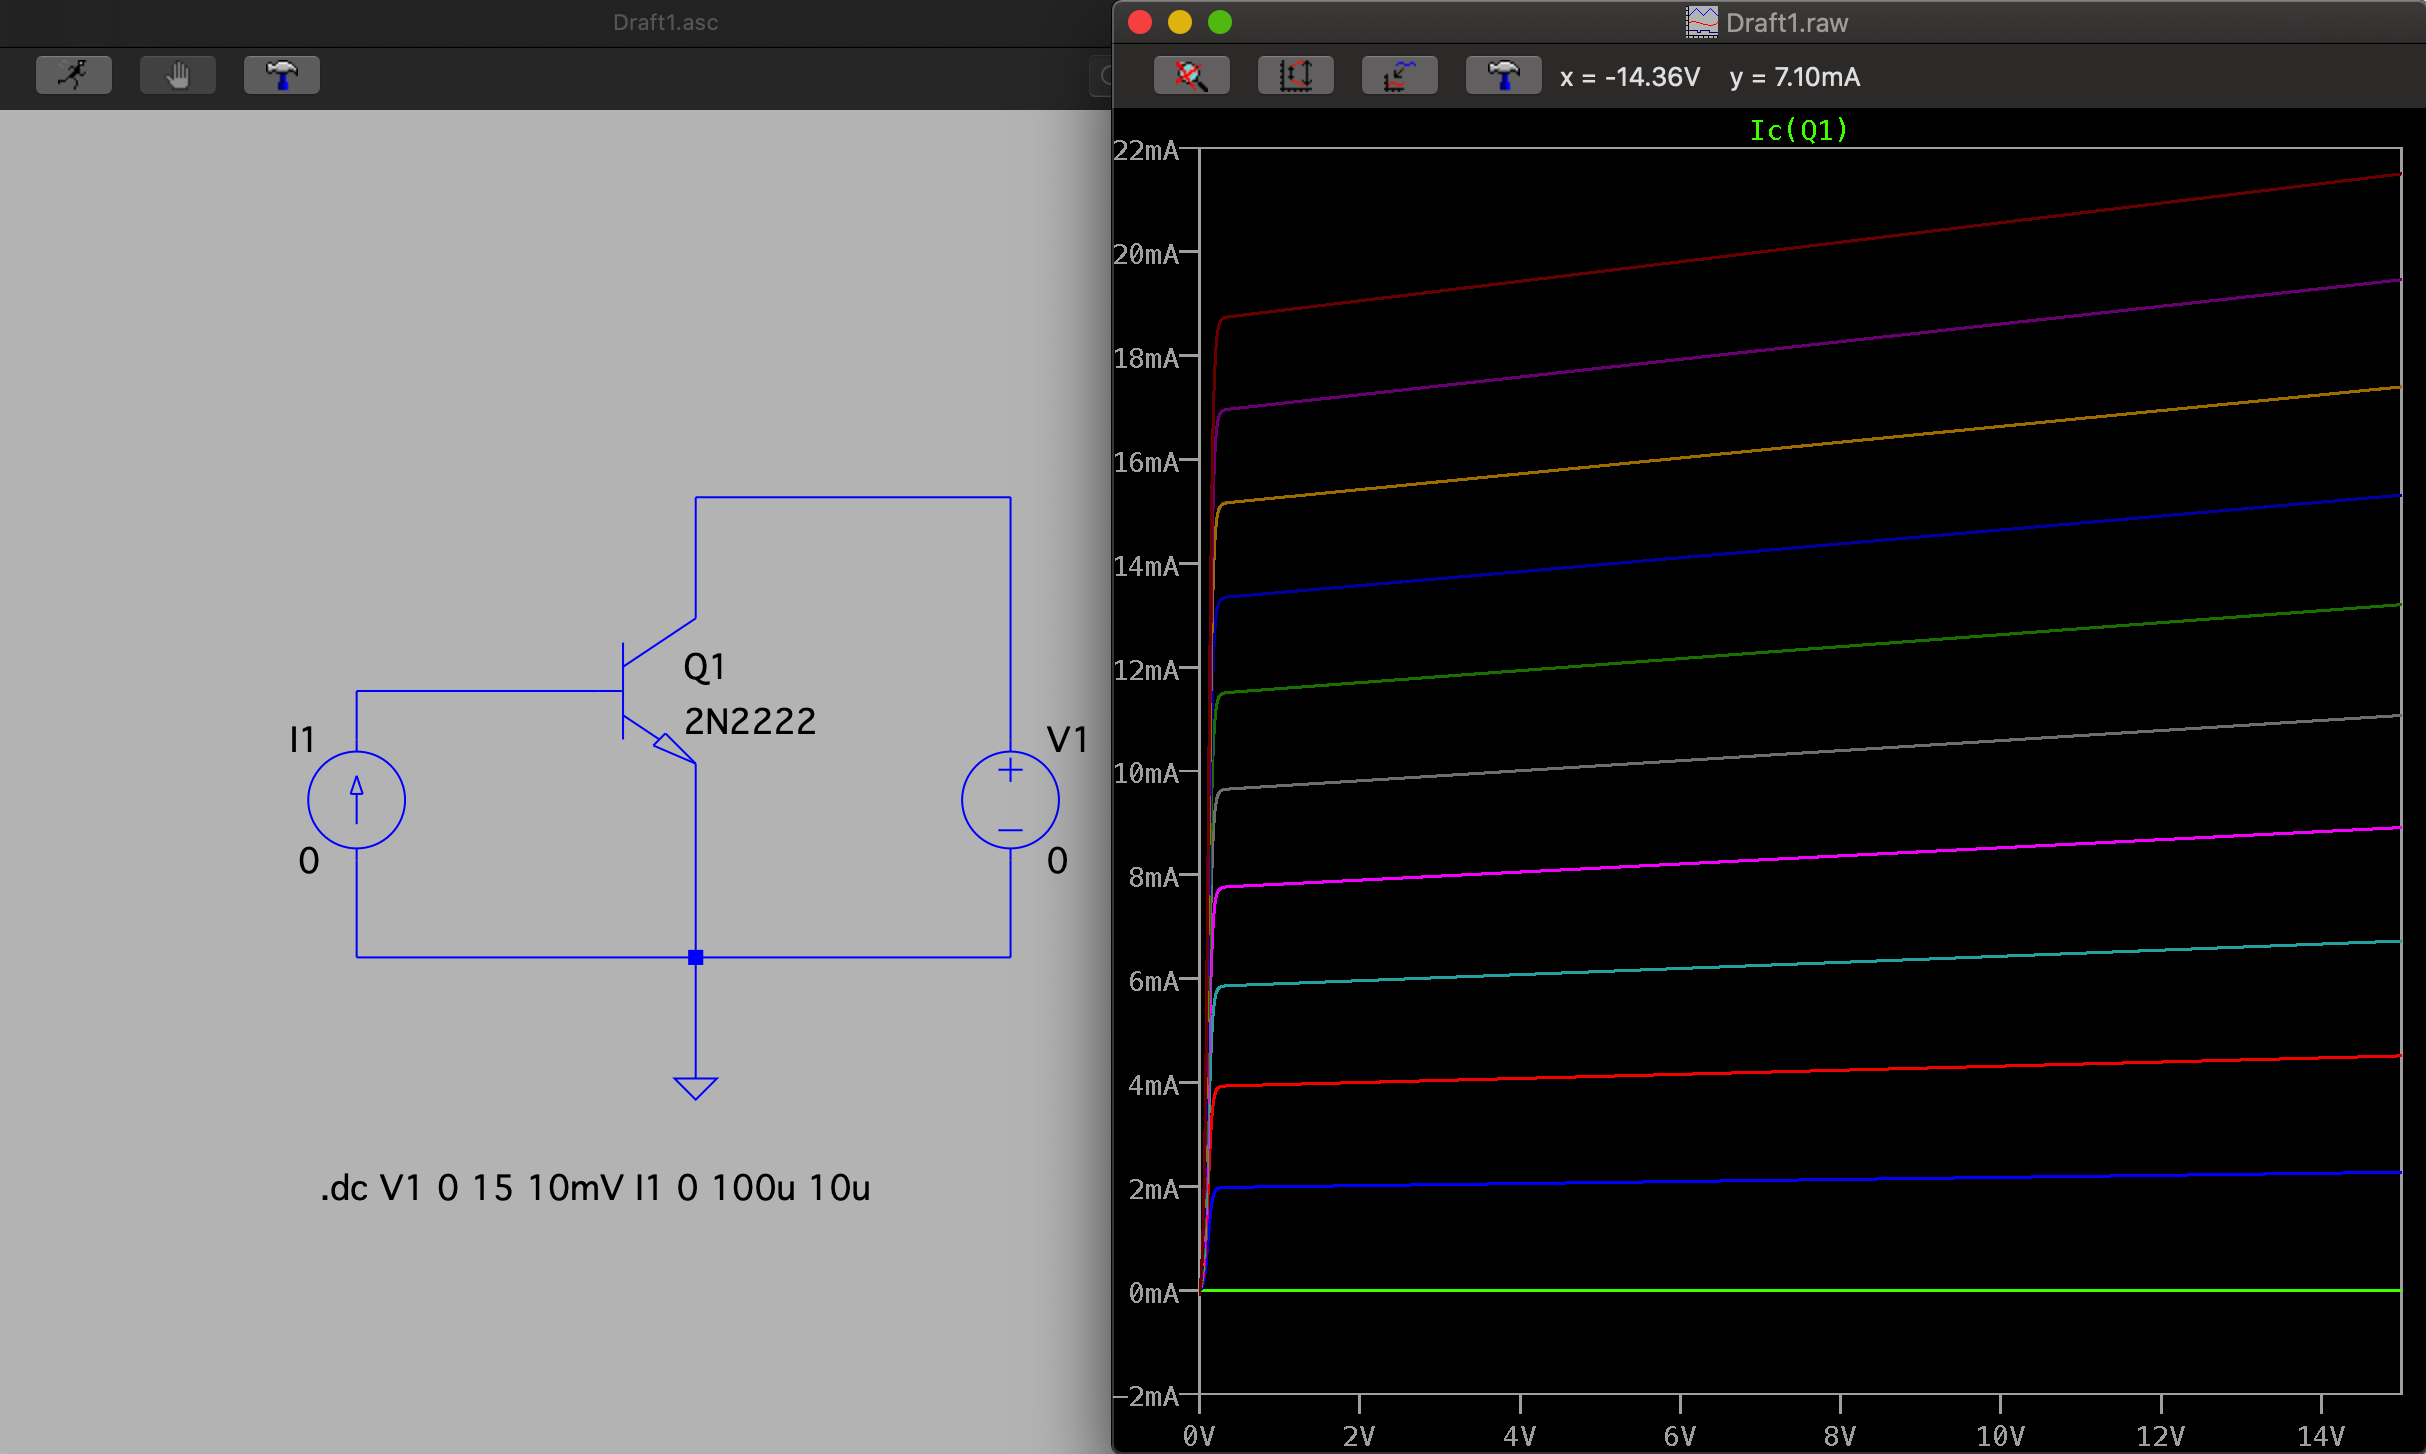
\includegraphics[width=\linewidth]{pictures/analysis_3.png}
          \end{minipage}
                                          &
          \begin{minipage}{.5\textwidth}
            \begin{itemize}
              \item Klickt auf 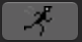
\includegraphics[scale=0.3]{pictures/run.png} (run) und LTspice startet die Simulation
              \item Wir wählen \textbf{IC(Q1)}, den Kollektorstrom.
            \end{itemize}
          \end{minipage}
          \\
        \end{tabular}
      \end{table}
    \end{tiny} \end{spacing}

  \begin{spacing}{0.9} \begin{tiny}
      \begin{table}[h!]
        \begin{tabular}{p{10cm} }
          \hline
          \textbf{Ergebnis und Auswertung} \\
          \hline                           \\
          Jeder Graph steht für einen simulierten Basisstrom. Per rechtem Mausklick $->$ View $->$ Steps könnt ihr einzelne Graphen zur
          detaillierten Analyse auswählen. \newline\newline Achtet darauf, welche Quelle ihr im $.dc ...$ simulation command zuerst wählt. \textbf{Quelle 1 ergibt im Diagramm die Abszisse, die Quelle 2 die Ordinate.}
        \end{tabular}
      \end{table}
    \end{tiny} \end{spacing}

\end{frame}

\begin{frame}[t]{NPN-Transistor}

  \begin{spacing}{0.6} \begin{tiny}

      Wenn ihr den Zusammenhang zwischen der Basisspannung $U_{be}$ und dem Kollektorstrom $I_c$ simulativ herausfinden wollt, müsst
      ihr die Schaltung leicht variieren. Dazu werden wir das schematic wie folgt anpassen.

    \end{tiny} \end{spacing}
  \begin{spacing}{0.9} \begin{tiny}
      \begin{table}[h!]
        \begin{tabular}{p{3cm} p{7cm}}
          \hline
          \textbf{Erstellung des Schaltplans}   & \\
          \hline                                  \\
          \begin{minipage}{.3\textwidth}
            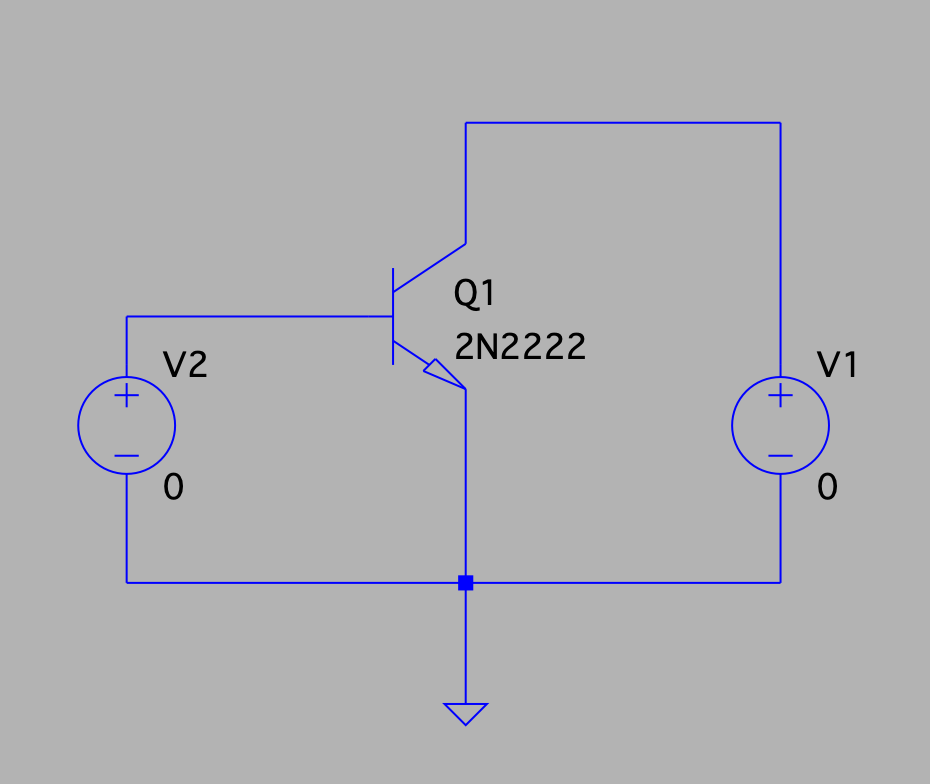
\includegraphics[width=\linewidth]{pictures/tran2.png}
          \end{minipage}
                                                &
          \begin{minipage}{.7\textwidth}
            \begin{itemize}
              \item Speichert das Projekt direkt als neue Datei ab (File $->$ save as )
              \item Löscht die Stromquelle (\textbf{F5}) und fügt eine Spannungsquelle hinzu.
              \item Verdrahtet die Schaltung wieder vollstänndig (\textbf{F3})
              \item Super simple dieses mal :)
            \end{itemize}
          \end{minipage}
          \\
                                                & \\
          \hline
          \textbf{Konfiguration der Simulation} & \\
          \hline                                  \\
          \begin{minipage}{.3\textwidth}
            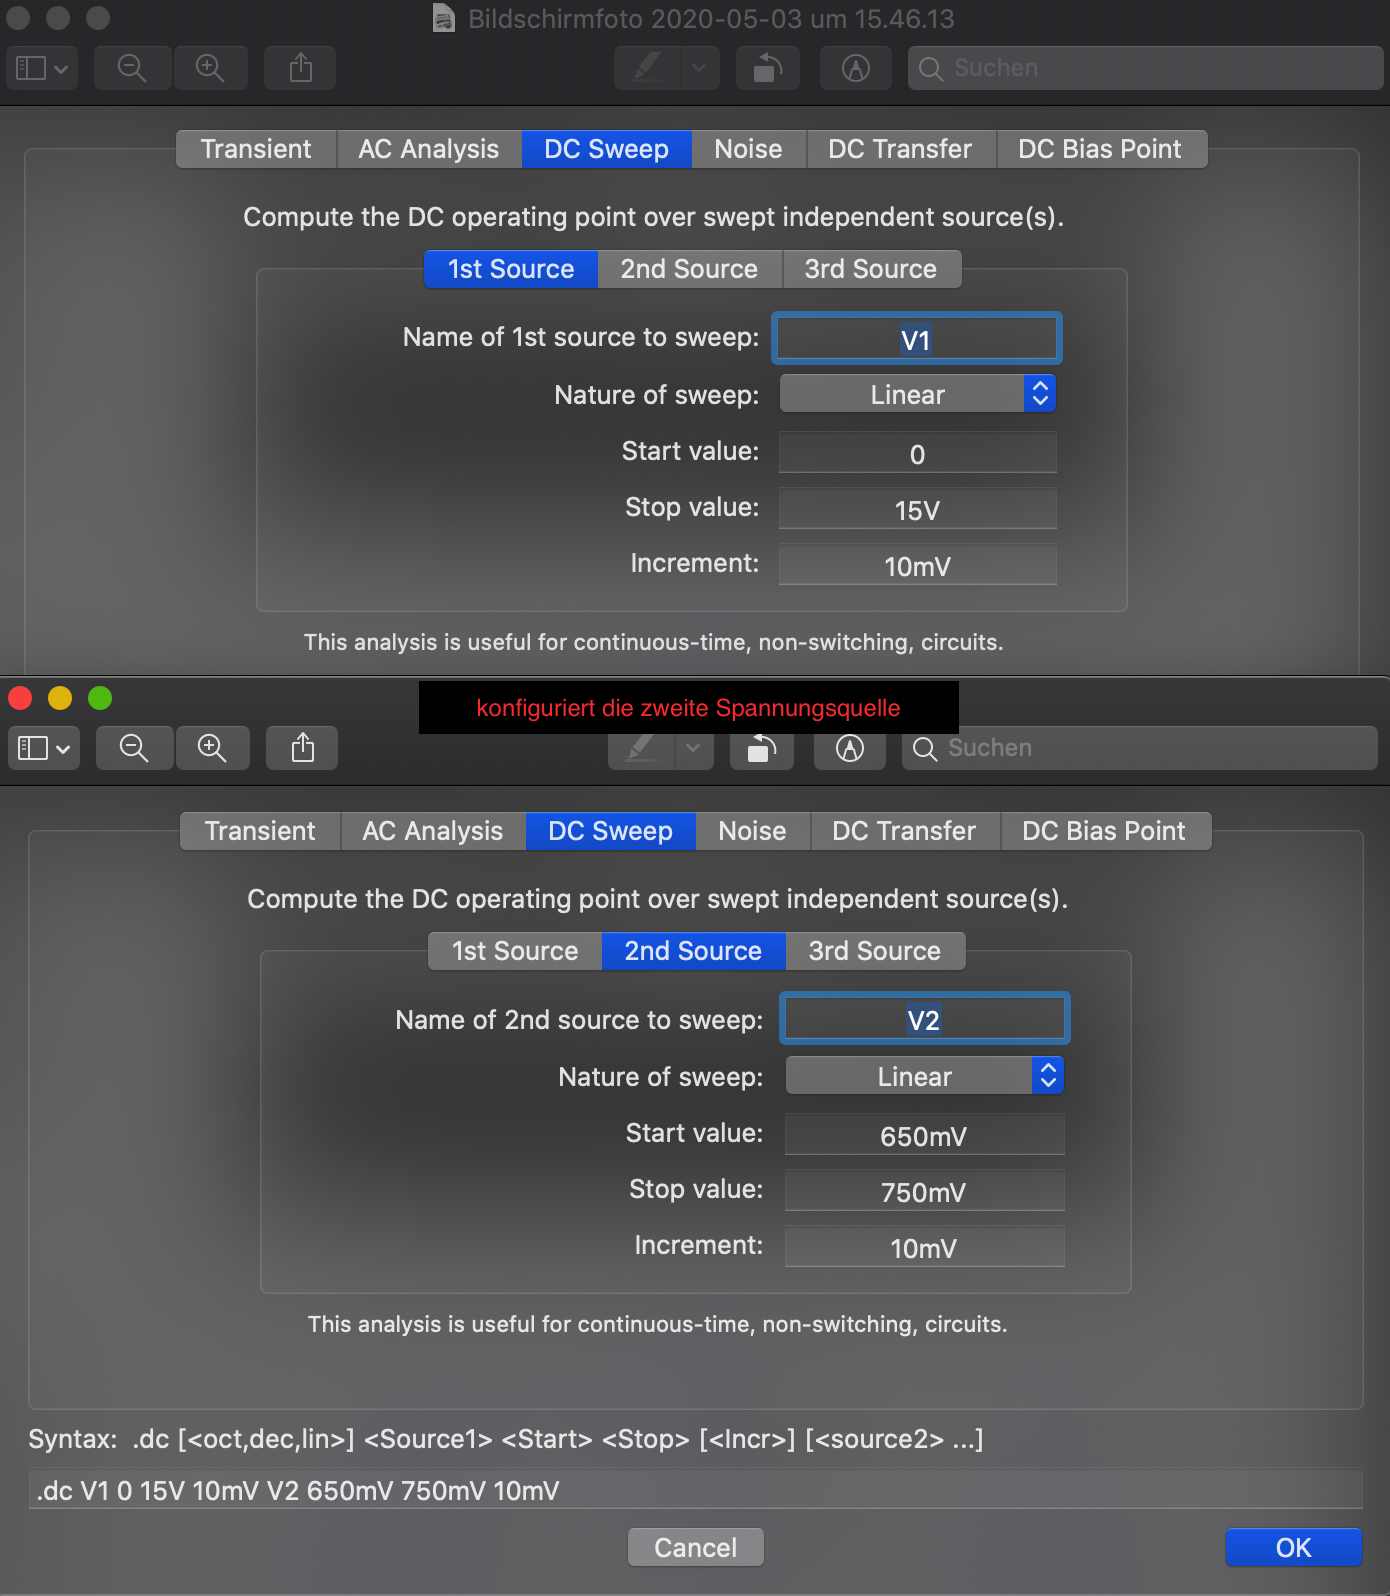
\includegraphics[width=0.8\linewidth]{pictures/simulationcmd_4.png}
          \end{minipage}
                                                &
          \begin{minipage}{.7\textwidth}
            \begin{itemize}
              \item Im Menu Simulation, wählt \textbf{Edit simulation command} und bliebt beim DC Sweep.
              \item Unser Ziel ist es das Ausgangskennlinienfeld des 2N2222 simlativ zu bestimmen. Dazu verwenden wir dieses mal
                    einen DC-Sweep mit einer Spannungsquelle, die die Basis-Emitterspannung $U_{be}$ simuliert und eine Spannungsquelle (V1) die die Spannung
                    $U_{ce}$ simuliert.
              \item V1 soll von 0 - 15V in 10mV Schritten simuliert werden, V2 von 650 - 750 mV in 10mV Schritten.
              \item Bestätigt mit \textit{OK} und fügt die Simlationsansweisung dem schematic hinzu
            \end{itemize}
          \end{minipage}
          \\
                                                & \\
          \hline
        \end{tabular}

      \end{table}

    \end{tiny} \end{spacing}

\end{frame}



\begin{frame}[t]{NPN-Transistor}

  \begin{spacing}{0.9} \begin{tiny}
      \begin{table}[h!]
        \begin{tabular}{p{5cm} p{5cm}}
          \hline
          \textbf{Simulation und Analyse} & \\
          \hline                            \\
          \begin{minipage}{.5\textwidth}
            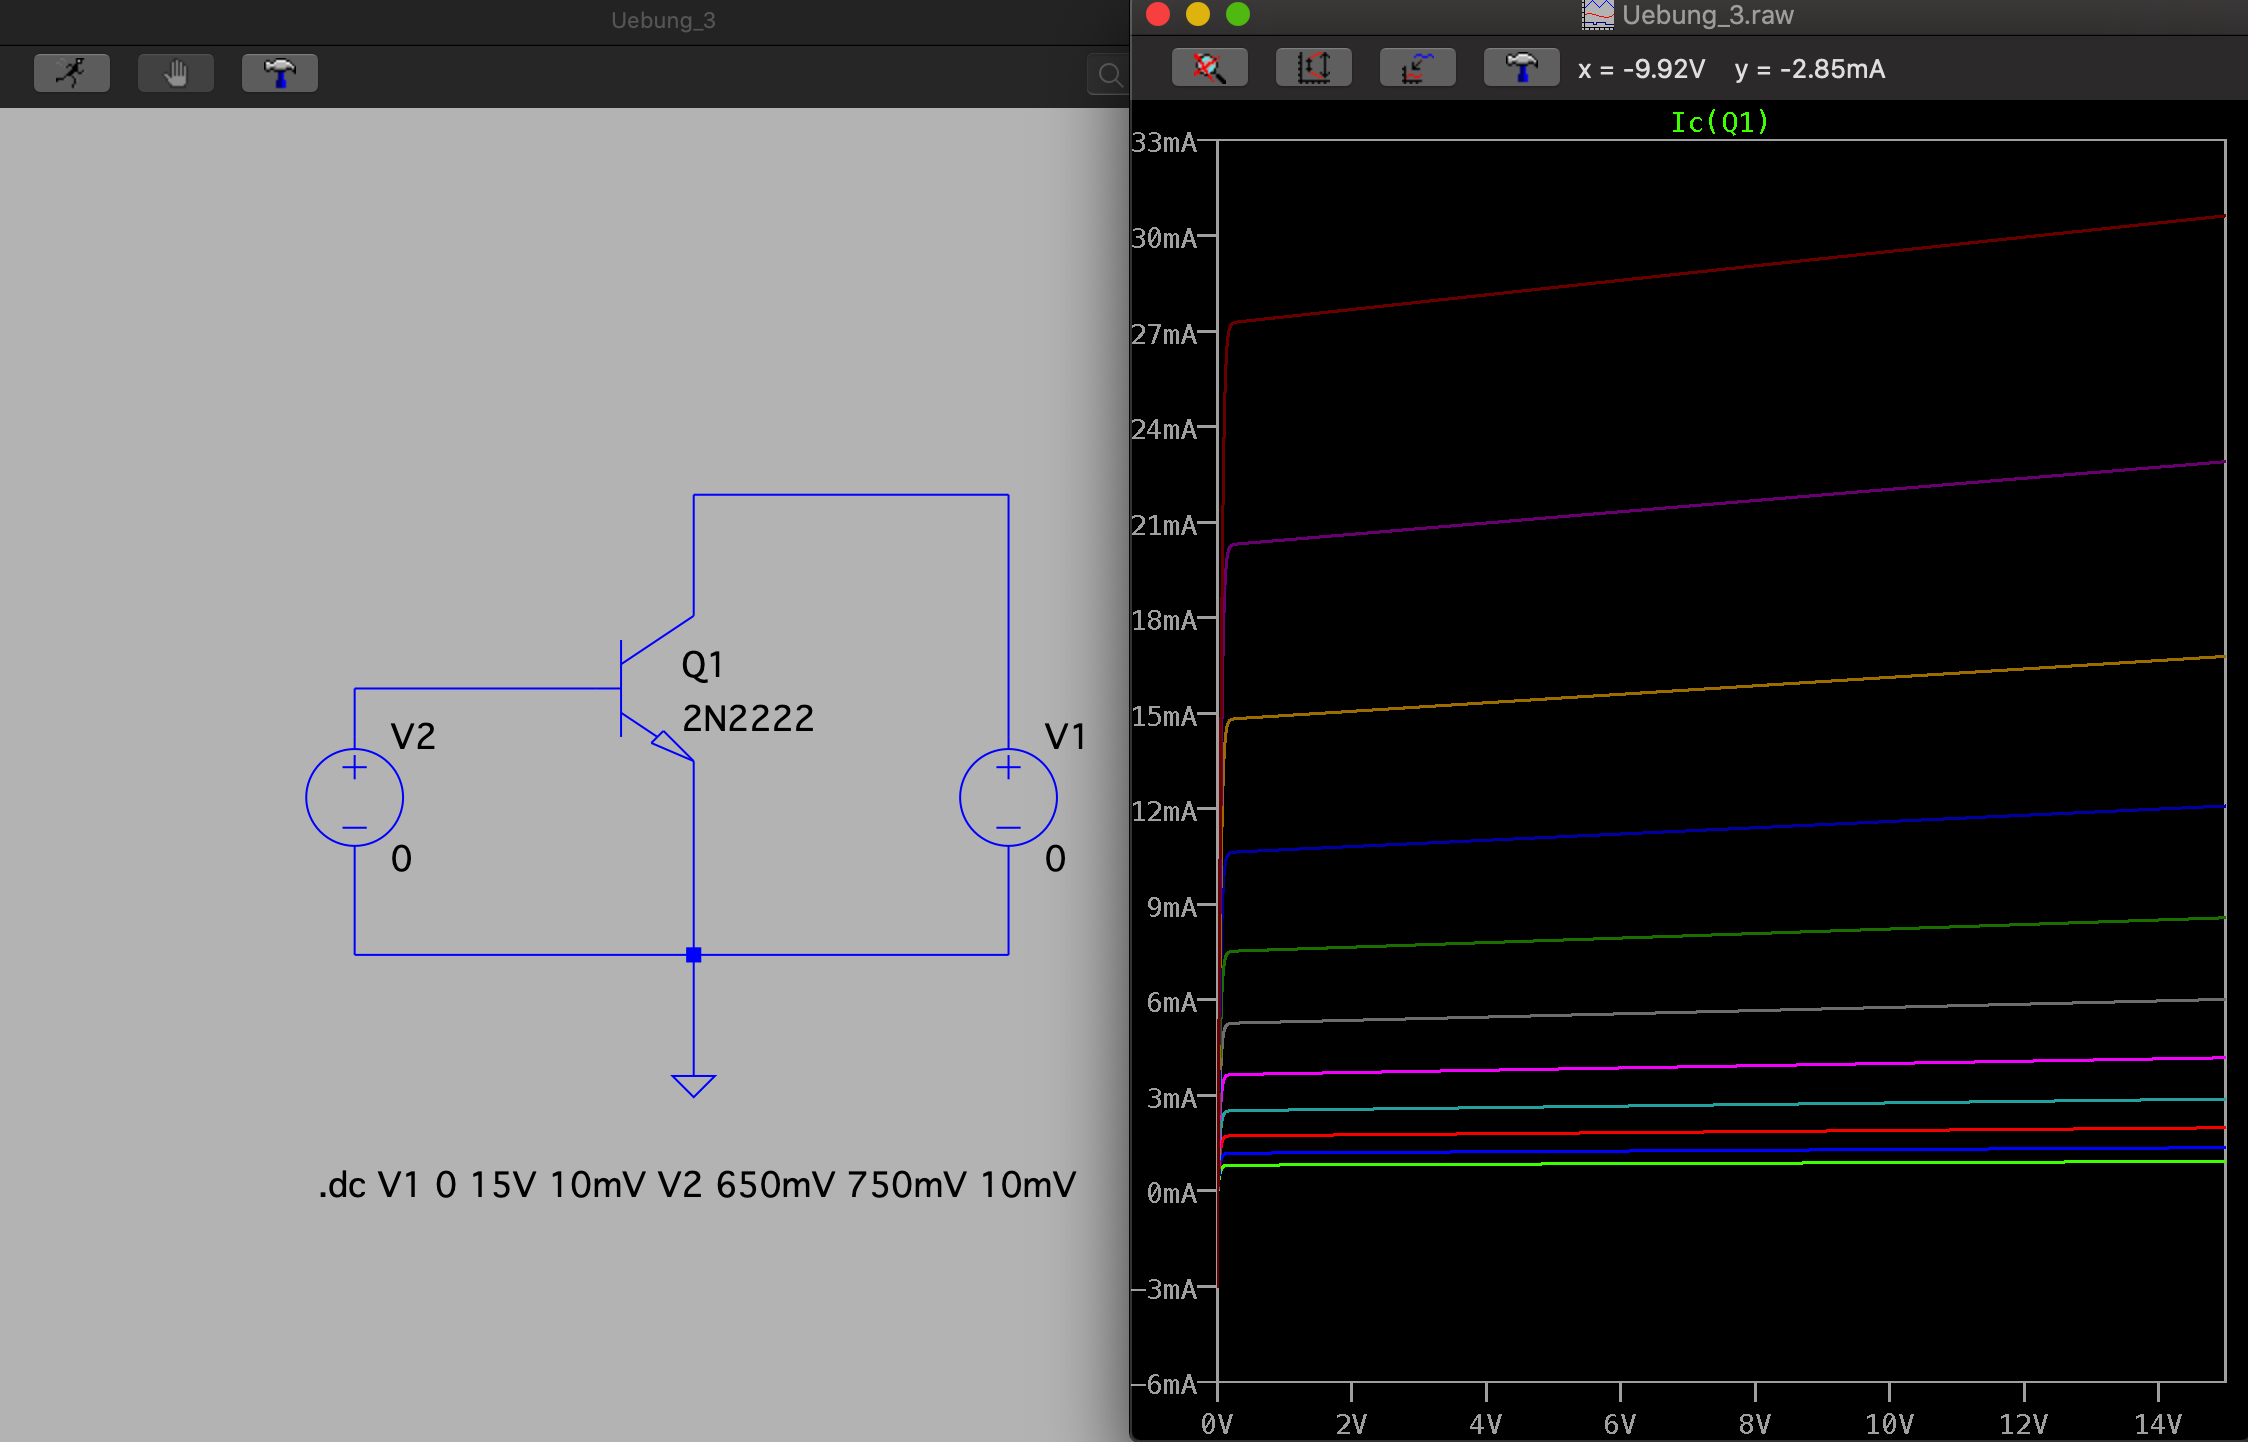
\includegraphics[width=\linewidth]{pictures/analysis_4.png}
          \end{minipage}
                                          &
          \begin{minipage}{.5\textwidth}
            \begin{itemize}
              \item Klickt auf 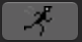
\includegraphics[scale=0.3]{pictures/run.png} (run) und LTspice startet die Simulation
              \item Wir wählen \textbf{IC(Q1)}, den Kollektorstrom.
            \end{itemize}
          \end{minipage}
          \\
        \end{tabular}
      \end{table}
    \end{tiny} \end{spacing}

  \begin{spacing}{0.9} \begin{tiny}
      \begin{table}[h!]
        \begin{tabular}{p{10cm} }
          \hline
          \textbf{Ergebnis und Auswertung} \\
          \hline                           \\
          Jeder Graph steht für eine simulierte $U_{be}$. Per rechtem Mausklick $->$ View $->$ Steps könnt ihr einzelne Graphen zur
          detaillierten Analyse auswählen. \newline\newline Achtet darauf, welche Quelle ihr im $.dc ...$ simulation command zuerst wählt. \textbf{Quelle 1 ergibt im Diagramm die Abszisse, die Quelle 2 die Ordinate.}
        \end{tabular}
      \end{table}
    \end{tiny} \end{spacing}

\end{frame}%transistor
\begin{frame}[t]{OPV Schaltungen - transient, ideal}

    \textbf{Ziel - Simulation eines invertierenden Verstärkers}
    
    \begin{spacing}{0.6} \begin{tiny}
    
    Wir wollen in einem einfachen simulativen Experiment die Funktionalität eines invertierenden Verstärkers nachvollziehen. 
    \begin{spacing}{0.9} \begin{tiny}
      \begin{table}[h!]
        \begin{tabular}{p{5cm} p{5cm}}
          \begin{minipage}{.5\textwidth}
            \begin{figure}
              \scalebox{0.35}{
            \centering
            \begin{circuitikz}
              \ctikzset{bipoles/length=1cm}
              \draw
              (0, 0) node[op amp] (opamp) {}
              (opamp.-) to[R,l_=$R_1$,-o] (-2, 0.35) -- (-3, 0.35) to [V=$v_1$] (-3,-0.5) to (-3,-0.5) node[ground]{}
              (opamp.-) to[short,*-] ++(0,0.5) coordinate (leftC)
              to[R=$R_2$] (leftC -| opamp.out)
              to[short,-*] (opamp.out) to [short,-o] (1.5,0) to (1.5,-0.5) node[ground]{}
              (opamp.+) -- (-1,-0.35) to (-1,-0.5) node[ground]{}
              ;
            \end{circuitikz}
              }
          \end{figure}
          \end{minipage} 
          & 
          \begin{minipage}{.5\textwidth}
          \begin{equation}
            V_{out}=-\frac{R2}{R1}V_{1}
            \end{equation}
          \end{minipage} 
        \end{tabular}
      
      \end{table}
      
      \end{tiny} \end{spacing}


  Wenn man nur daran interessiert ist die grundsätzliche Funktionalität einer Schaltung zu verifizieren, kann man ideale
  Bauelemente aus der LTspice Bibliothek verwenden. Wie im obigen Beispiel benötigt z.B. der Operationsverstärker entgegen der Realität dann keine Spannungsversorgung.
  Für einen idealen OPV bietet LTspice das Bauelement \textbf{opamp} an, welches Ihr im Bauteileditor findet direkt über die Suche findet. \newline
  \textbf{Wichtig:} Ihr müsst als Spice-Direktive jedoch noch ein zu verwendendes Model einbinden. (.lib opamp.sub)
    \end{tiny} \end{spacing}
    \begin{spacing}{0.9} \begin{tiny}
    \begin{table}[h!]
      \begin{tabular}{p{3cm} p{7cm}}
        \hline
        \textbf{Erstellung des Schaltplans} & \\
        \hline \\
        \begin{minipage}{.3\textwidth}
          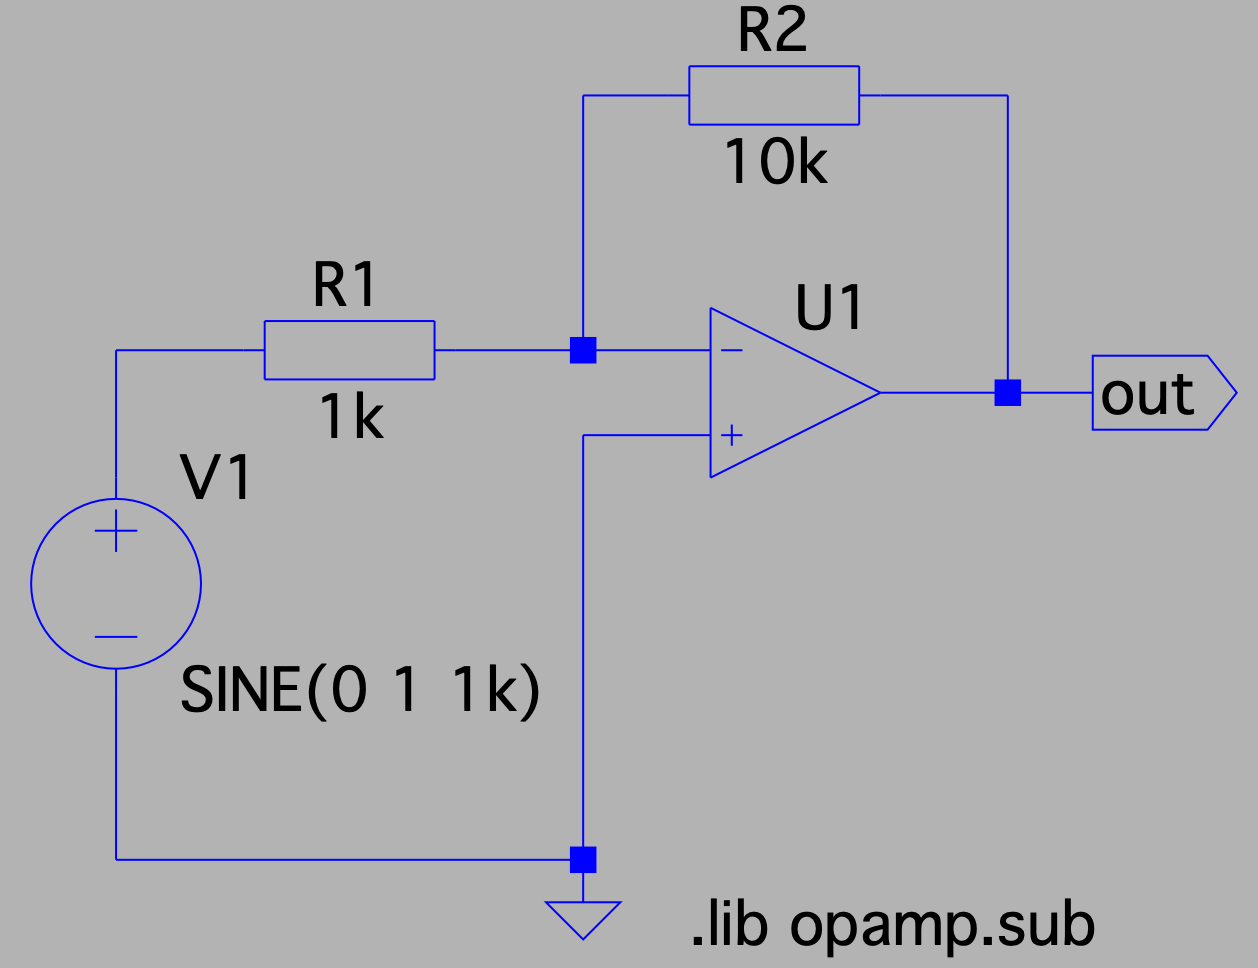
\includegraphics[width=0.8\linewidth]{pictures/opamp_1.png}
        \end{minipage} 
        & 
        \begin{minipage}{.7\textwidth}
        \begin{itemize}
          \item Baut den Schaltplan mit dem o.g. opamp als OPV auf. 
          \item Über einen rechten Mausklick kommt ihr ins \textbf{Advanced} Menü der Spannungsquelle. Hier könnt ihr Sie als Signalgenerator konfigurieren. Wir wählen einen \textbf{Sinus mit 1V Amplitude und der Frequenz 1kHz}
          \item Die library kann direkt als spice directive eingebunden werden (siehe Folie 5, .op)
          \item Ihr könnt über die Funktion \textbf{Label Net (F4)} einen Knoten umbennen und ihm mit einem Symbol für In-/Output versehen. Nennt den Ausgang der Schaltung z.B. \textit{out}.
          \item \textbf{Hinweis:} Wenn ihr einen Knoten benennt, dann kann liegt unter diesem Namen überall im Schaltplan das selbe! Potential an. 
          Dadurch könnt ihr den Plan übersichtlicher gestalten. 
        \end{itemize}
        \end{minipage} 
        \\
         & \\
         \hline
      \end{tabular}
    
    \end{table}
    
    \end{tiny} \end{spacing}
    
     \end{frame}
    
     \begin{frame}[t]{OPV Schaltungen - transient, ideal}
    
      \begin{spacing}{0.9} \begin{tiny}
      \begin{table}[h!]
        \begin{tabular}{p{4cm} p{6cm}}
          \hline
          \textbf{Konfiguration der Simulation} & \\
          \hline \\
          \begin{minipage}{.3\textwidth}
           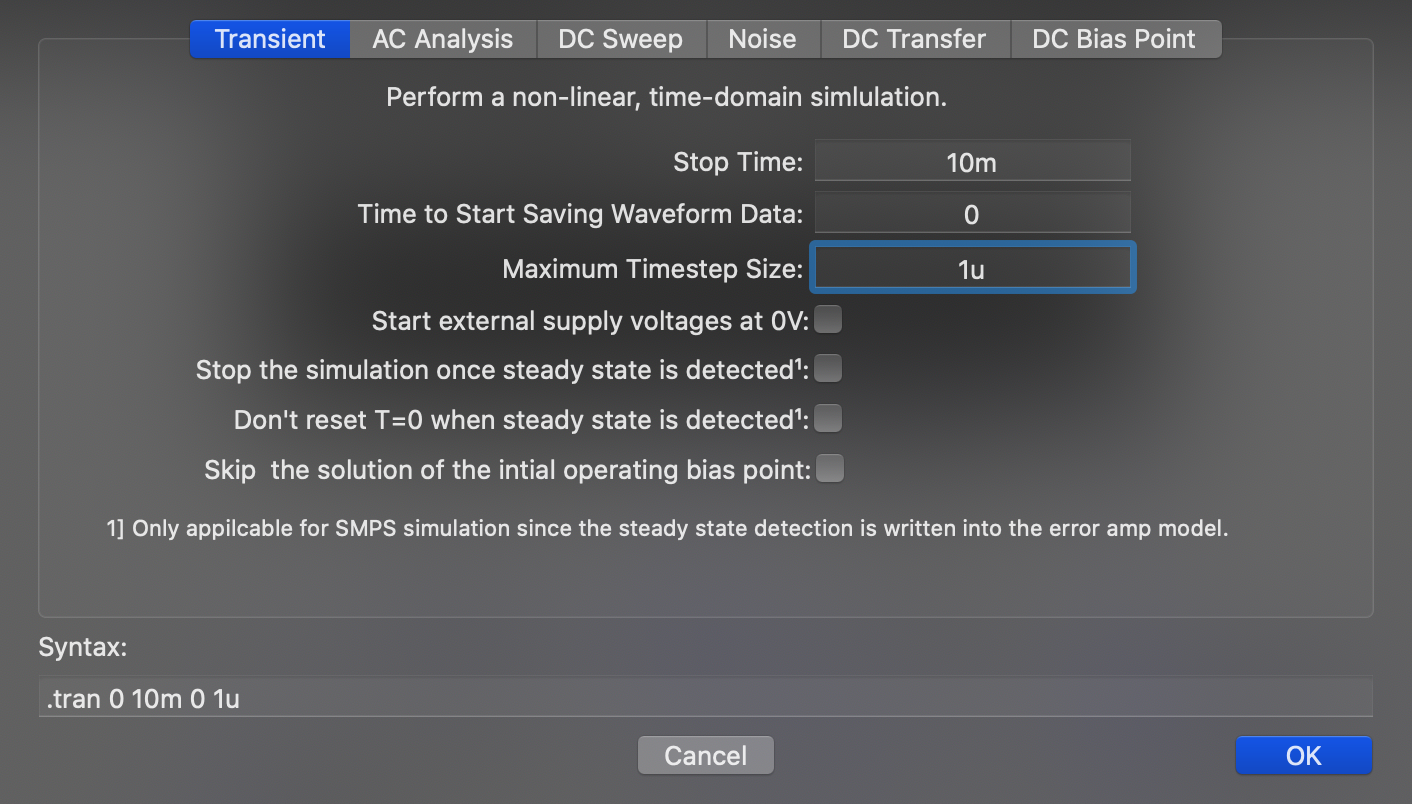
\includegraphics[width=\linewidth]{pictures/simulationcmd_5.png}
         \end{minipage} 
         & 
         \begin{minipage}{.7\textwidth}
         \begin{itemize}
           \item Im Menu Simulation, wählt \textbf{Edit simulation command} und wählt eine \textbf{Transient} Analyse. 
           \item Unser Ziel ist es am Ausgang eine Verstärkte Spannung entsprechend des Verstärkungsfaktors der Schaltung zu messen.
           \item Da die Schaltung ideal kein Einschwingverhalten zeigt, starten wir direkt mit der Aufzeichnung und simulieren 10ms mit einer Schrittweite von 10us.
           \item Bestätigt mit \textit{OK} und fügt die Sumlationsansweisung dem schematic hinzu
         \end{itemize}
         \end{minipage} 
         \\
          & \\
          \hline
          \textbf{Simulation und Analyse} & \\
          \hline \\
          \begin{minipage}{.5\textwidth}
            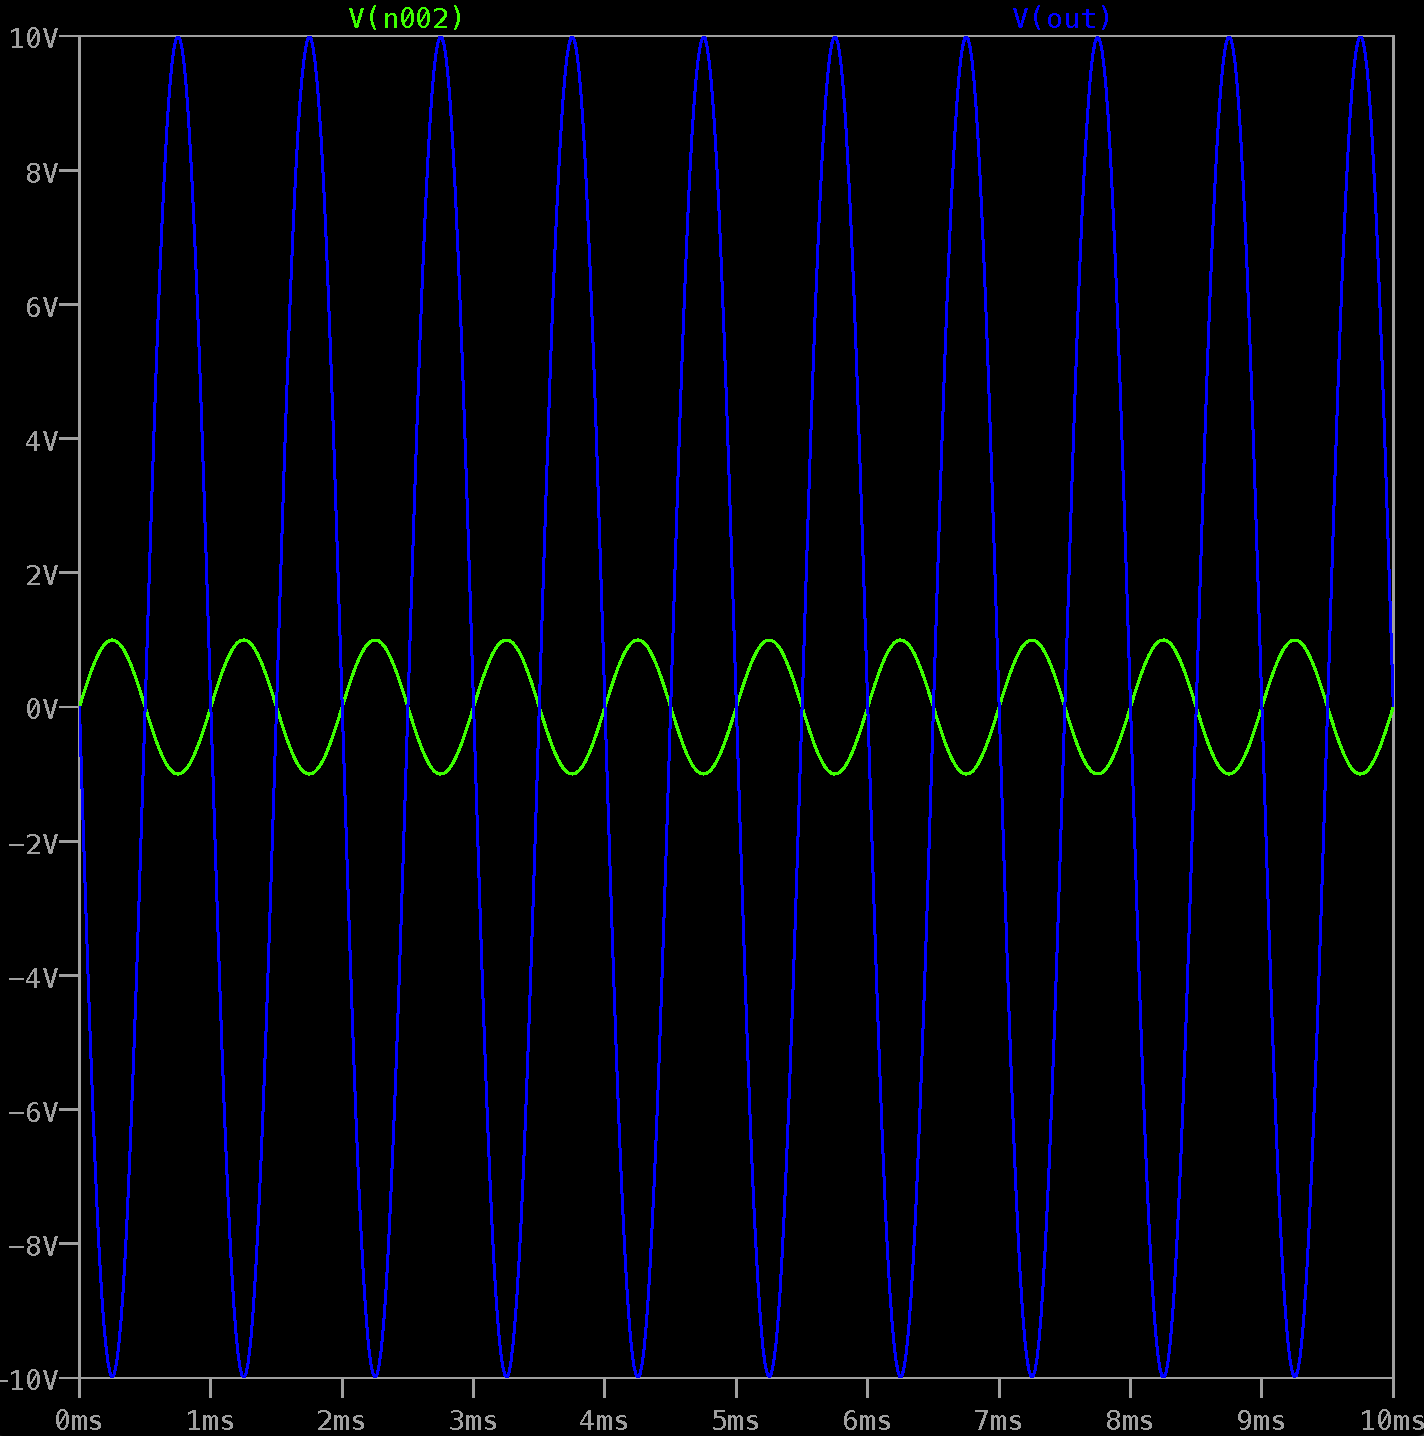
\includegraphics[width=0.5\linewidth]{pictures/analysis_5.png}
          \end{minipage} 
          & 
          \begin{minipage}{.5\textwidth}
          \begin{itemize}
            \item Klickt auf 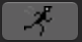
\includegraphics[scale=0.3]{pictures/run.png} (run) und LTspice startet die Simulation
            \item Fügt nun die Eingangsspannung sowie die Ausgangsspannung der Schaltung als Messpunkte hinzu.
          \end{itemize}
          \end{minipage} 
          \\
        \end{tabular}
      \end{table}
    \end{tiny} \end{spacing}
    
      \begin{spacing}{0.9} \begin{tiny}
        \begin{table}[h!]
          \begin{tabular}{p{10cm} }
            \hline
            \textbf{Ergebnis und Auswertung} \\
            \hline \\    
            Verifiziert, ob die Verstärkung sowie das invertierende Verhalten zu eurem Erwartungswert (10) passt. 
          \end{tabular}
        \end{table}
      \end{tiny} \end{spacing}
      
       \end{frame}

       \begin{frame}[t]{OPV Schaltungen - transient, nicht ideal}

        \begin{spacing}{0.6} \begin{tiny}
        Im nächsten Experiment wollen wir die gleiche Schaltung mit einem "nicht idealen" Verstärken simulieren und die Verwendung
        von Labels verdeutlichen. 
        \end{tiny} \end{spacing}
  
        \begin{spacing}{0.9} \begin{tiny}
        \begin{table}[h!]
          \begin{tabular}{p{3cm} p{7cm}}
            \hline
            \textbf{Erstellung des Schaltplans} & \\
            \hline \\
            \begin{minipage}{.3\textwidth}
              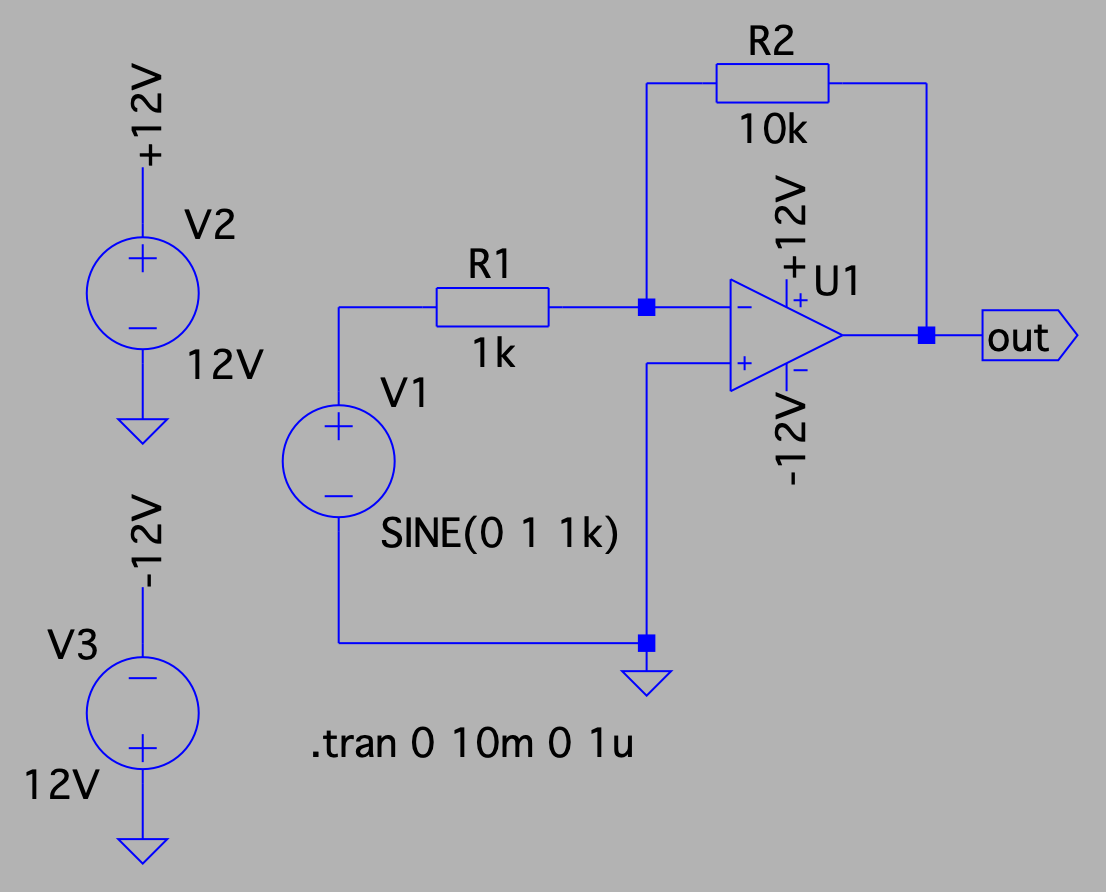
\includegraphics[width=0.8\linewidth]{pictures/opamp_2.png}
            \end{minipage} 
            & 
            \begin{minipage}{.7\textwidth}
            \begin{itemize}
              \item Tauscht den opamp gegen das Bauteil \textbf{UniversalOpamp2} aus dem Bauteileditor (\textbf{F2}).
              \item Fügt zwei neue Spannungsquellen für die Versorgung des OPV's hinzu. 
              \item Achtet hierbei auf darauf, dass die Label wirklich auf dem Potential +12V und -12V liegen.
              \item Erstellt die Labels +12V und -12V (\textbf{Label Net (F4)}).
            \end{itemize}
            \end{minipage} 
            \\
          \end{tabular}

        \end{table}
        
        \end{tiny} \end{spacing}

                    
      \begin{spacing}{0.9} \begin{tiny}
        \begin{table}[h!]
          \begin{tabular}{p{10cm} }
            \hline
            \textbf{Ergebnis und Auswertung} \\
            \hline \\    
            Es muss das selbe Ergebnis herauskommen wie im vorherigen Experiment unter Verwendung des idealen OPV's \textbf{opamp}.
          \end{tabular}
        \end{table}
      \end{tiny} \end{spacing}
        
         \end{frame}


       \begin{frame}[t]{OPV Schaltungen - Analyse der Grenzfrequenz einer Schaltung }

        \begin{spacing}{0.6} \begin{tiny}
        Eine Kennzahl von Tief-/Hochpassfiltern ist ihre 3dB Grenzfrequenz $f_g$. Die Grenzfrequenz kann man analytisch, jedoch auch simulativ
        über LTspice bestimmen. Hierzu bietet LTspice die Möglichkeit die Frequenz einer Schaltung zu variieren. Dies wird AC-Sweep genannt. 
        Im Bode-Diagramm kann man den logarithmischen Verlauf der Amplitude über der Frequenz in LTspice darstellen und 
        somit einfach grafisch die Grenzfrequenz bestimmen indem man den Punkt heraussucht, bei dem die Amplitde um 3dB abgefallen ist.
        \end{tiny} \end{spacing}
  
        \begin{spacing}{0.9} \begin{tiny}
          \begin{table}[h!]
            \begin{tabular}{p{10cm}}
              \hline
              \textbf{Erstellung des Schaltplans + Konfiguration der Simulation} \\
              \hline     
            \end{tabular}
          \begin{tabular}{p{2cm} p{2cm} p{6cm}}
            \begin{minipage}{.2\textwidth}
              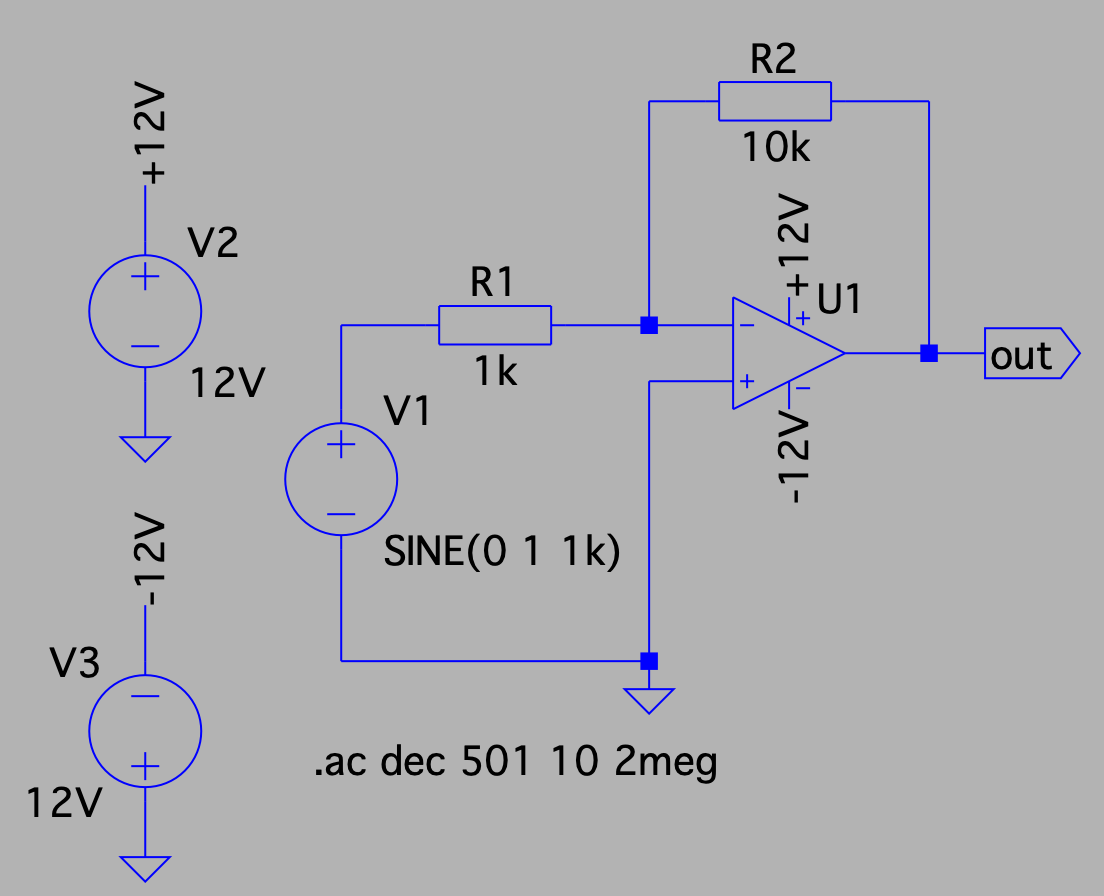
\includegraphics[width=0.8\linewidth]{pictures/opamp_3.png}
            \end{minipage} 
            &  
            \begin{minipage}{.2\textwidth}
              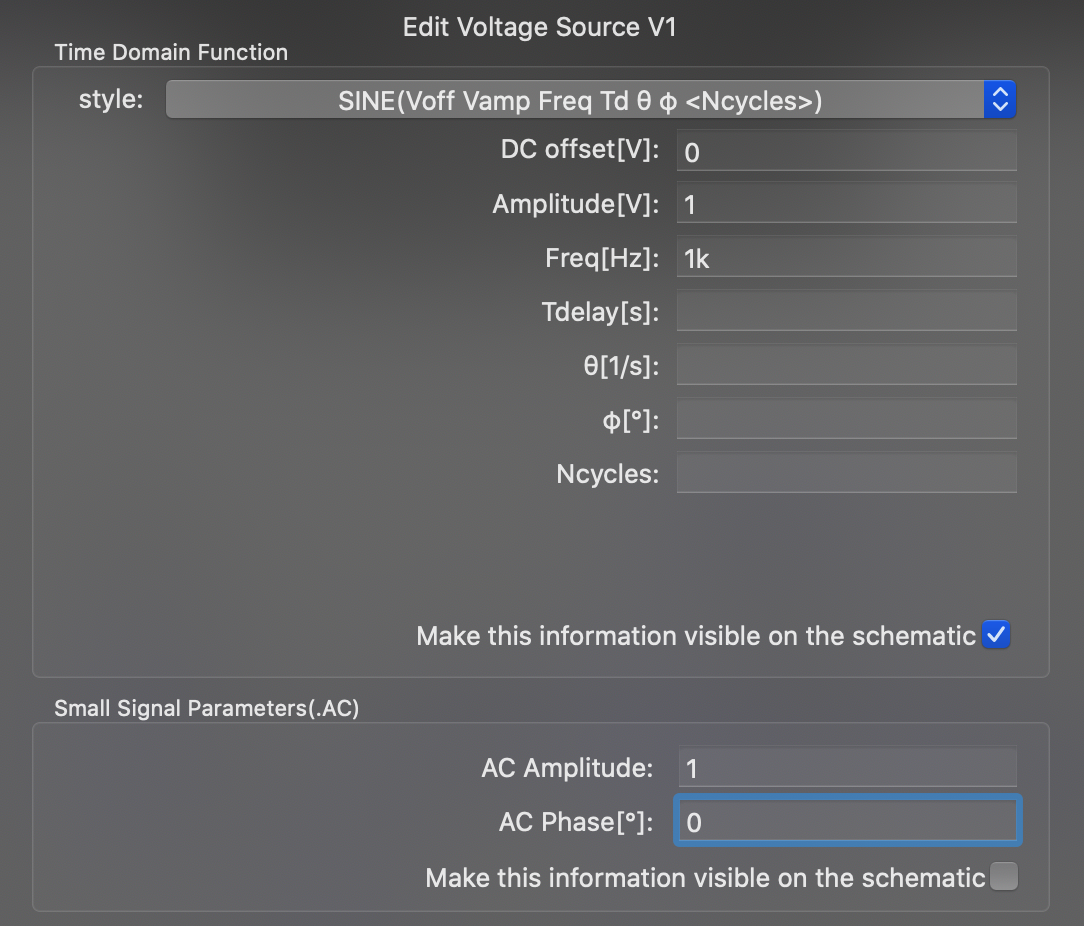
\includegraphics[width=0.8\linewidth]{pictures/ac_small_signal.png}
            \end{minipage} 
            & 
            \begin{minipage}{.5\textwidth}
            \begin{itemize}
              \item Wir verwenden die Schaltung aus dem vorherigen Beispiel!
              \item Wichtig ist hierbei, dass wir Spannungsquelle für den AC-Sweep konfigurieren
              Hierzu geht ihr per rechtem Mausklick in das advanced menu von V1 und stellt das Kleinsignal Verhalten (AC)
              auf \textbf{Amplitude 1V und Frequenz 1kHz}.
            \end{itemize}
            \end{minipage} 
            \\
          \end{tabular}
          \begin{tabular}{p{6cm} p{4cm}}
            \hline
            \textbf{Simulation und Analyse} & \\
            \hline \\
            \begin{minipage}{.6\textwidth}
              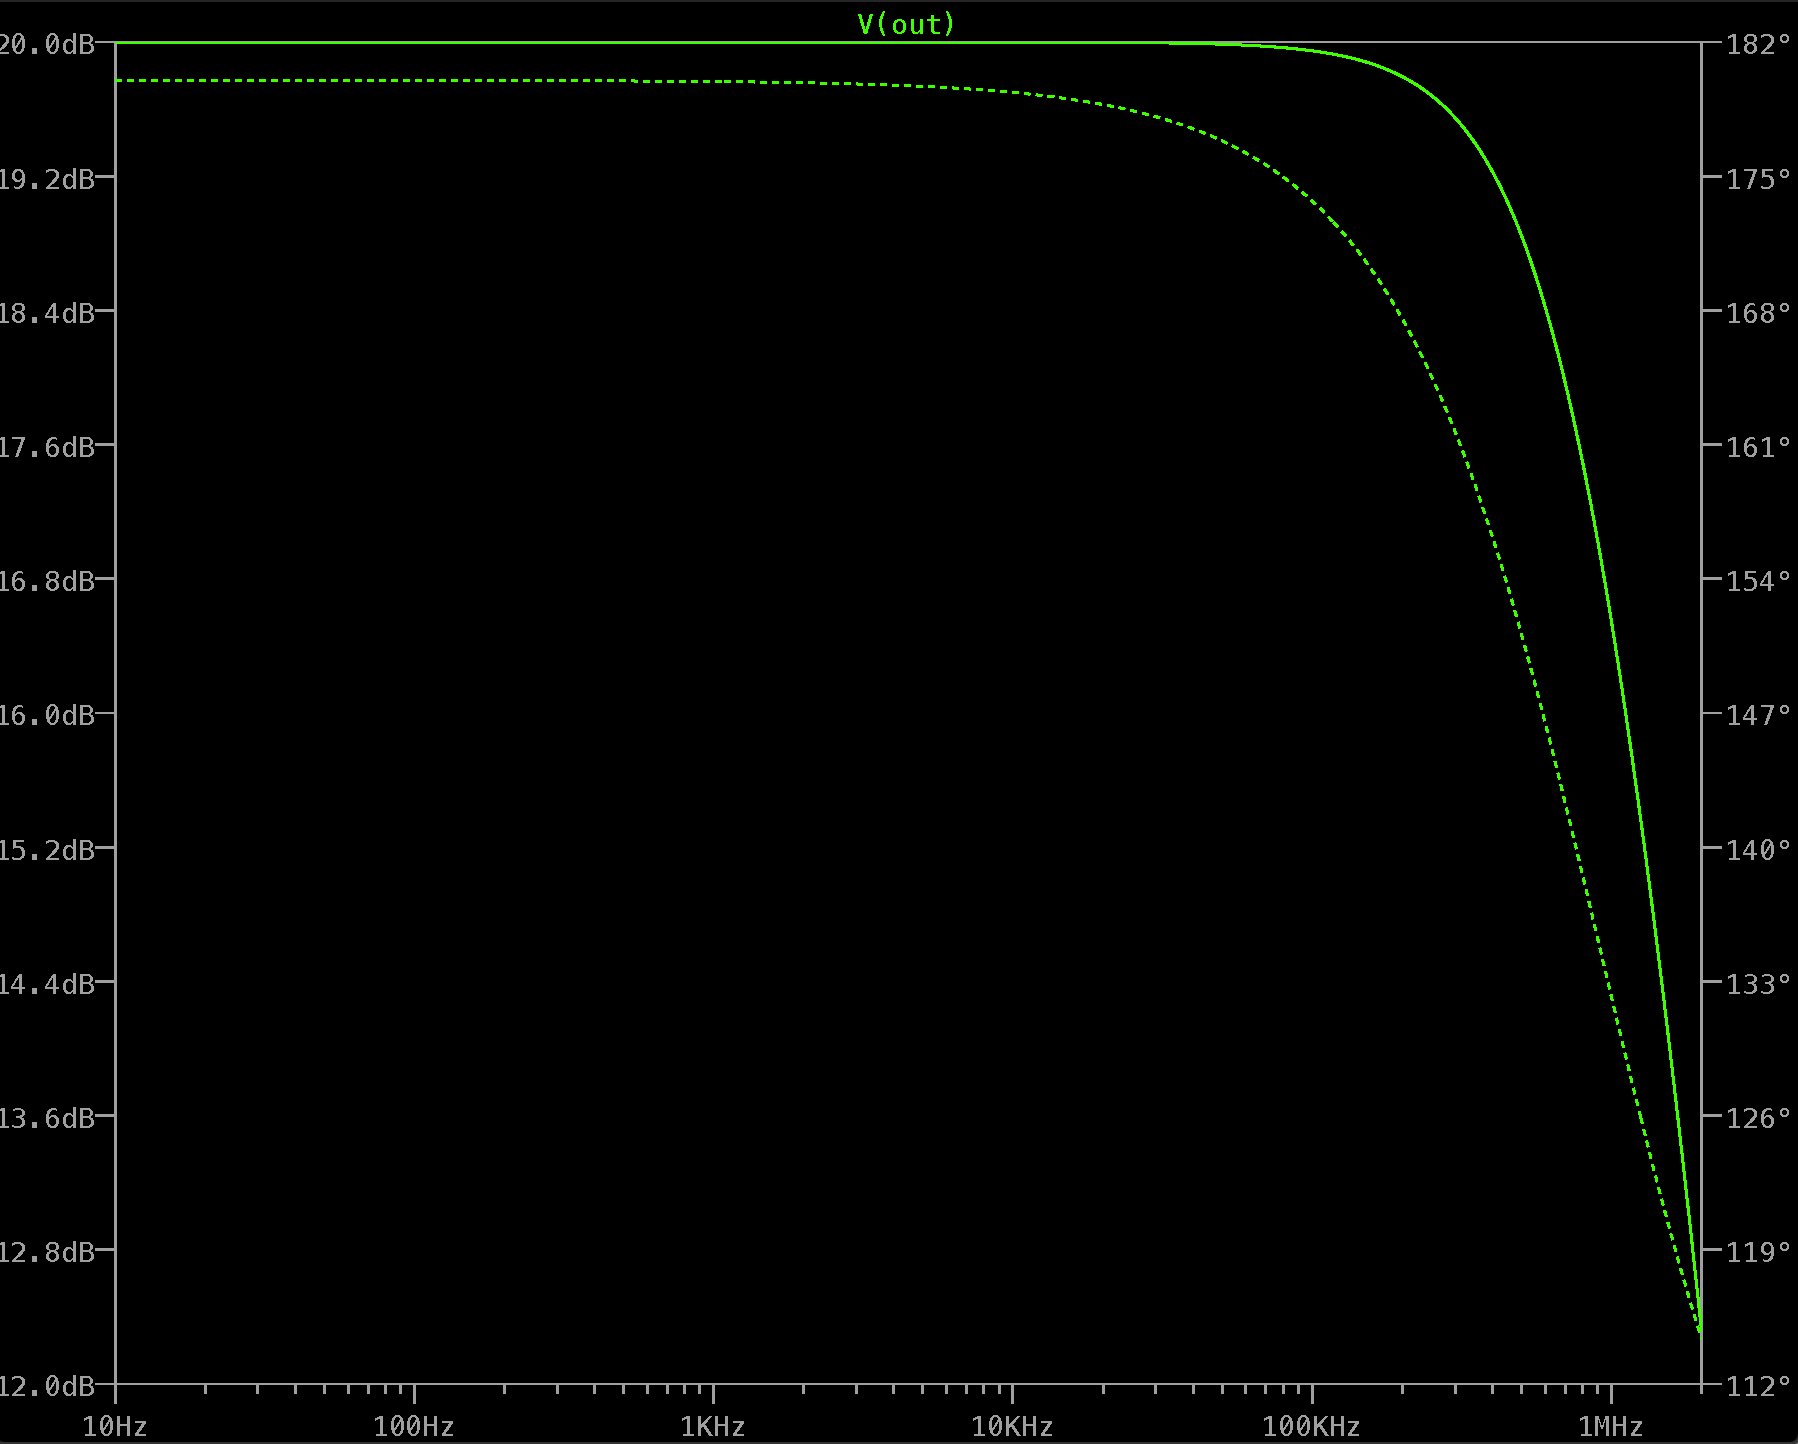
\includegraphics[width=0.7\linewidth]{pictures/analysis_6.png}
            \end{minipage} 
            & 
            \begin{minipage}{.4\textwidth}
            \begin{itemize}
              \item Klickt auf 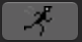
\includegraphics[scale=0.3]{pictures/run.png} (run) und LTspice startet die Simulation
              \item Fügt nun die Ausgangsspannung der Schaltung als Messpunkt hinzu.
              \item Im waveform viewer solltet ihr das Bode-Diagram mit Amplitude und Phase sehen.
            \end{itemize}
            \end{minipage} 
            \\
          \end{tabular}

        \end{table}
        
        \end{tiny} \end{spacing}

                    
      %\begin{spacing}{0.9} \begin{tiny}
      %  \begin{table}[h!]
      %    \begin{tabular}{p{10cm} }
      %      \hline
      %      \textbf{Ergebnis und Auswertung} \\
      %      \hline \\    
      %      Es muss das selbe Ergebnis herauskommen wie im vorherigen Experiment unter Verwendung des idealen OPV's \textbf{opamp}.
      %    \end{tabular}
      %  \end{table}
      %\end{tiny} \end{spacing}
        
         \end{frame}

         \begin{frame}[t]{OPV Schaltungen - Analyse der Grenzfrequenz einer Schaltung }
    
          \begin{spacing}{0.9} \begin{tiny}
            \begin{table}[h!]
            \begin{tabular}{p{10cm}}
              \hline
              \textbf{Simulation und Analyse} \\
              \hline \\
              \begin{minipage}{\textwidth}
                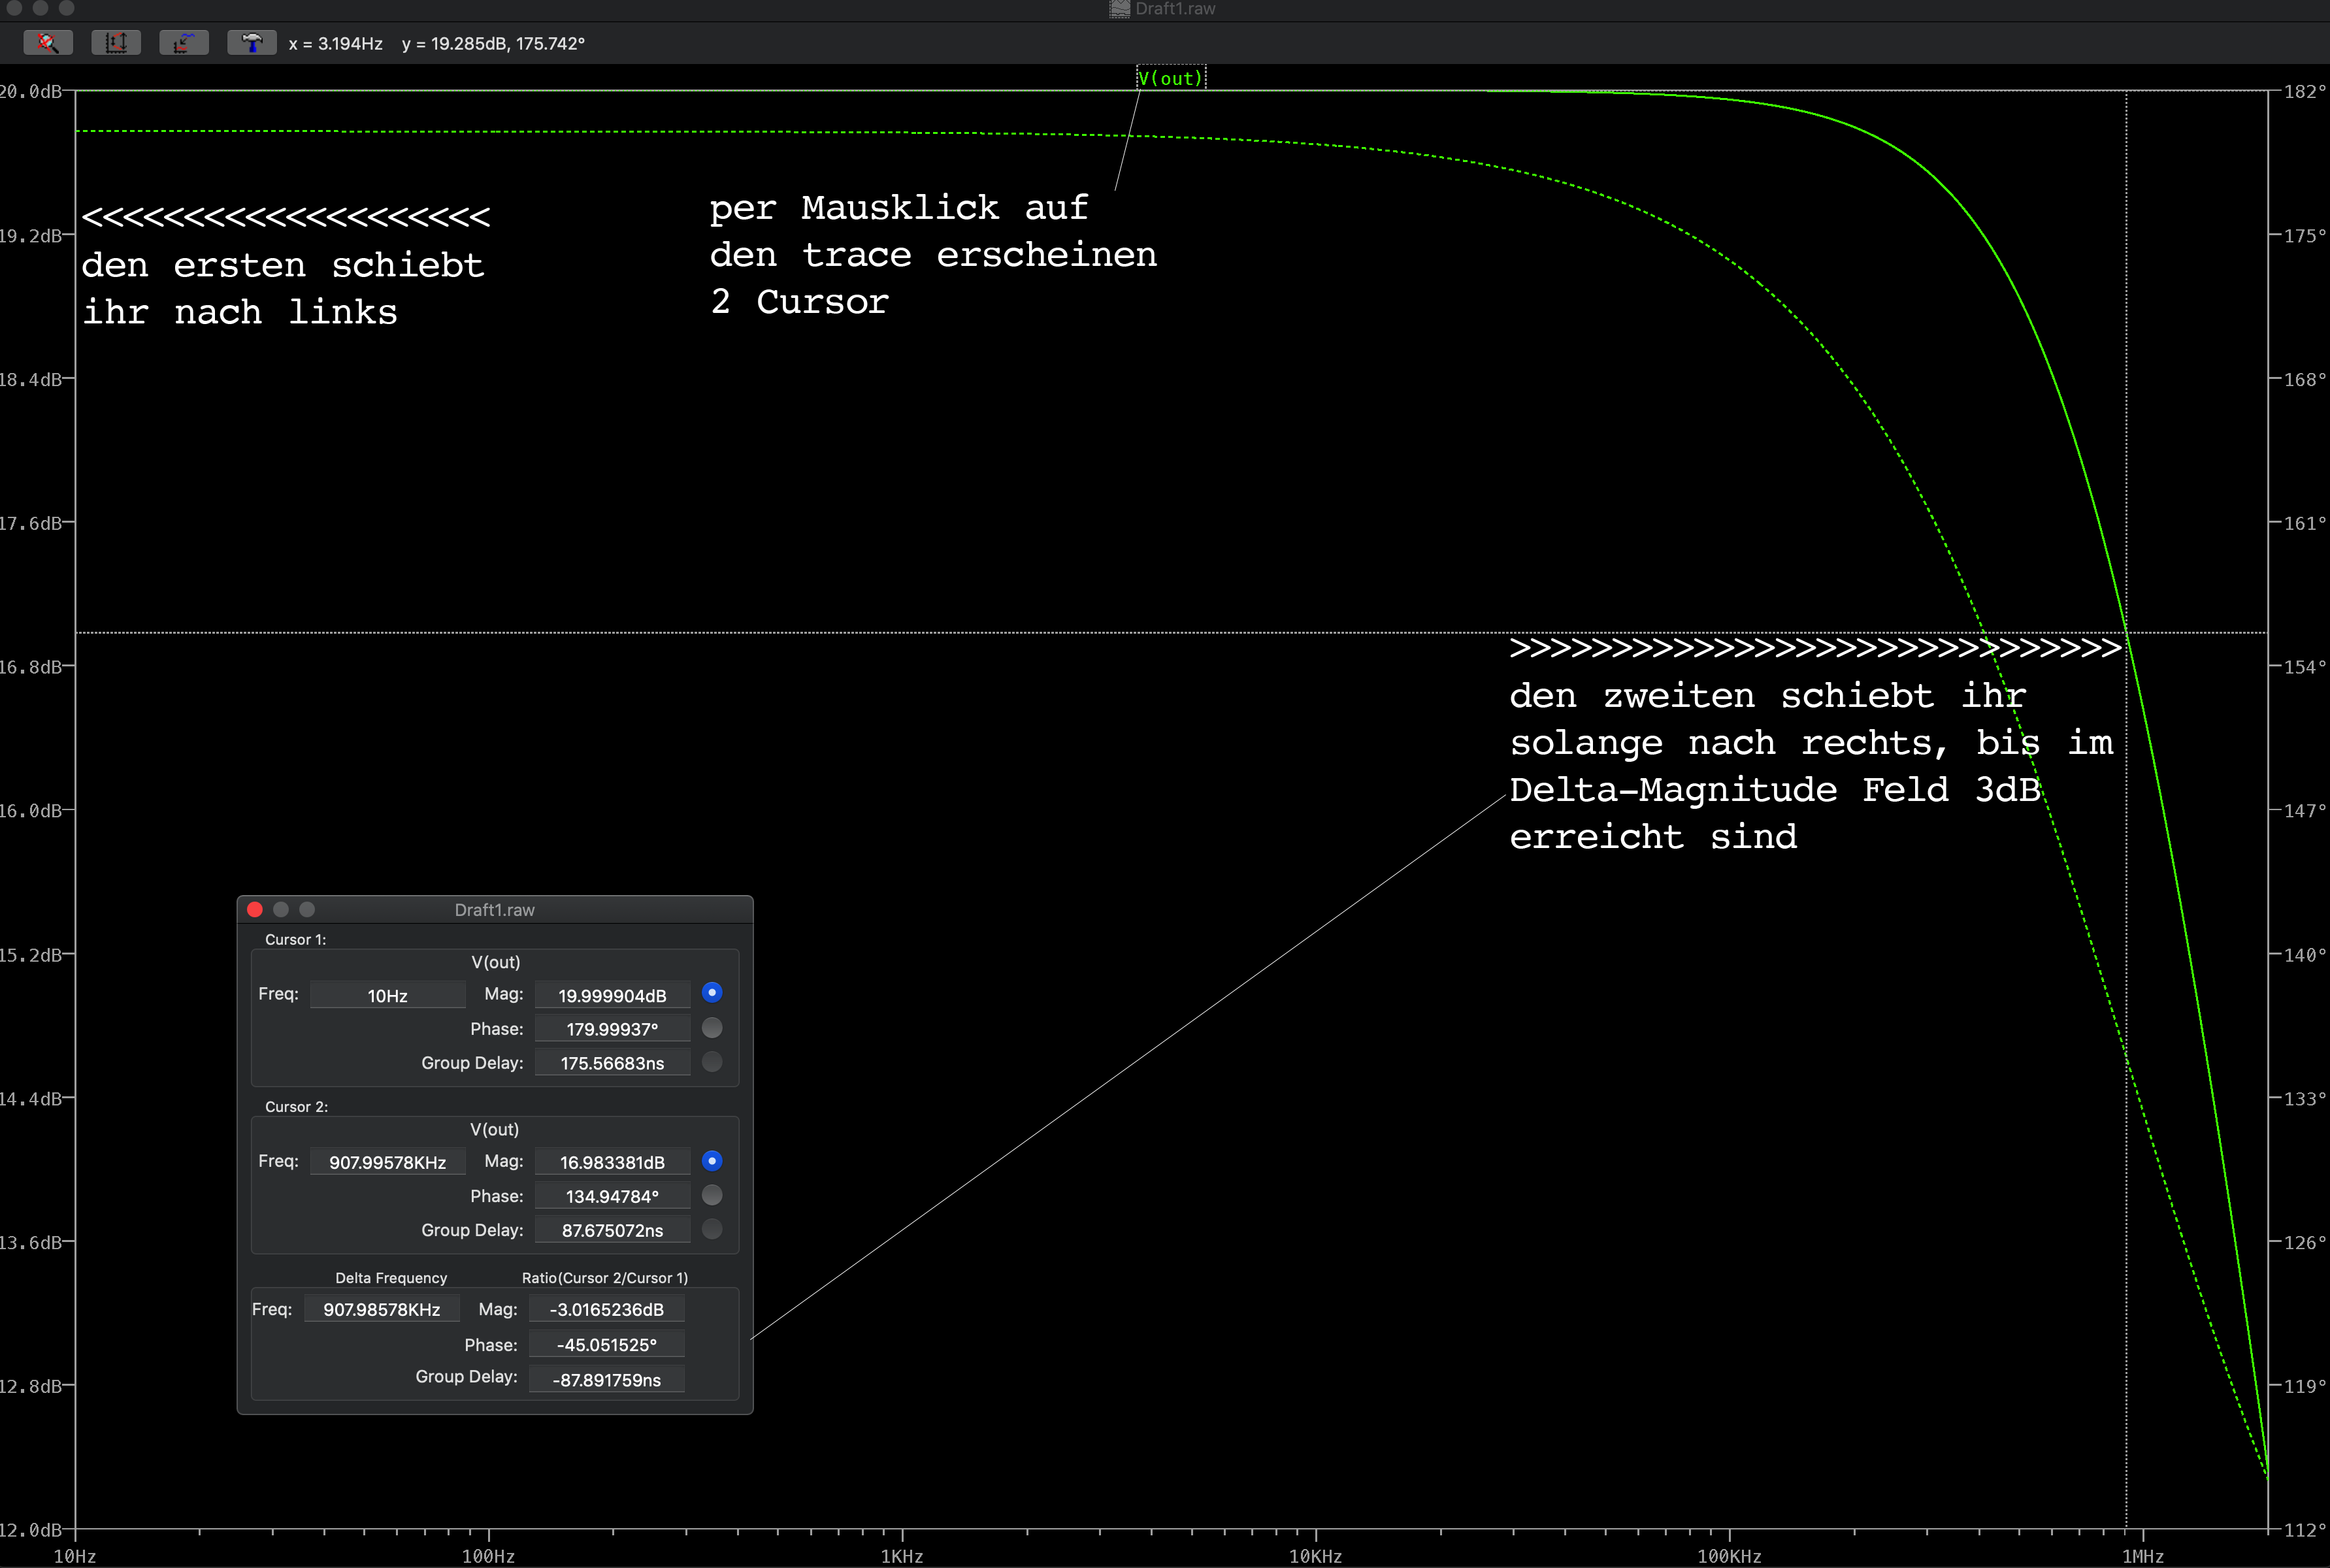
\includegraphics[width=\linewidth]{pictures/bode_1_remastered.png}
              \end{minipage} 
              \\
            \end{tabular}
  
          \end{table}
           
          \end{tiny} \end{spacing}
   
                      
        %\begin{spacing}{0.9} \begin{tiny}
        %  \begin{table}[h!]
        %    \begin{tabular}{p{10cm} }
        %      \hline
        %      \textbf{Ergebnis und Auswertung} \\
        %      \hline \\    
        %      Es muss das selbe Ergebnis herauskommen wie im vorherigen Experiment unter Verwendung des idealen OPV's \textbf{opamp}.
        %    \end{tabular}
        %  \end{table}
        %\end{tiny} \end{spacing}
          
           \end{frame}


         \begin{frame}[t]{OPV Schaltungen - nicht-invertierender Verstärker}

          \textbf{Ziel - Anwendung der Kenntnisse}
    
          \begin{spacing}{0.6} \begin{tiny}
          
          Nachfolgend könnt ihr die Schaltung für einen nicht-invertierenden Verstärker in einer OPV Schaltung sehen. 

          \begin{enumerate}
            \item Baut die Schaltung auf, dimensioniert sie so, dass Sie einen Verstärkungsfaktor
            \item Verwendet die UniversalOpamp2 aus der vorherigen Übrung mit einer Versorgungsspannung von +/-12V
            \item Verifiziert eure Schaltung und das \textbf{nicht-invertierende} Verhalten mit einer transienten Simulation von 0 - 50ms.
            \item Wählt dabei eine ausreichend kleine Schrittweite
            \item Wechselt die Simulationsart zum AC-Sweep und ermittelt die Grenzfrequenz
          \end{enumerate}

            \begin{table}[h!]
              \begin{tabular}{p{5cm} p{5cm}}
                \begin{minipage}{.5\textwidth}
                  \begin{figure}
                    \scalebox{0.35}{
                  \centering
                  \begin{circuitikz}
                    \ctikzset{bipoles/length=1cm}
                    \draw
                    (0,0) node[op amp,yscale=-1](opamp){} 
                    (opamp.+) to[short,-o] ++ (-2,0) to [V=$v_1$] ++ (0,-3) to ++(0,0) node[ground] {}
                    (opamp.-) to[short] ++ (0,-1.25) coordinate(X) to[R,l_=$R_1$] ++(0,-1) node[ground]{}
                    (opamp.out) to[R,l_=$R_2$] ++ (0,-1.5) coordinate(Y) to[short] ++ (-1.7,0) coordinate(X){}
                    (opamp.out) to[short,*-o] ++ (0.5,0) node[right]{$v_{\rm out}$}
                    ;
                    \end{circuitikz} 
                    }
                    
                \end{figure}
                \end{minipage} 
                & 
                \begin{minipage}{.5\textwidth}
                \begin{equation}
                  V_{out}=(1+\frac{R2}{R1})V_{1}
                  \end{equation}
                \end{minipage} 
              \end{tabular}
            
            \end{table}

            Spoiler! - Die Lösungen folgen auf den folgenden Folien. Wenn sie sich nicht sicher sind, schauen Sie einfach nach.\newline\newline
            Info! - Besonders die Analyse von Grenzfrequeznen ist für Ihre weitere Vorlesungzeit (Filter höhrerer Ordnung, EMV) hilfreich,
            da Sie neben der simulativen Bestätigung Ihrer Schaltungen auch theoretische Rechenaufgaben simulieren und so Ihre Rechnung
            verifizieren können.
            
            \end{tiny} \end{spacing}
           \end{frame}

          \begin{frame}[t]{OPV Schaltungen - Lösung transient}

              \begin{spacing}{0.9} \begin{tiny}
                \begin{table}[h!]
                \begin{tabular}{p{10cm}}
                  \hline
                  \textbf{Simulation und Analyse} \\
                  \hline \\
                  \begin{minipage}{\textwidth}
                    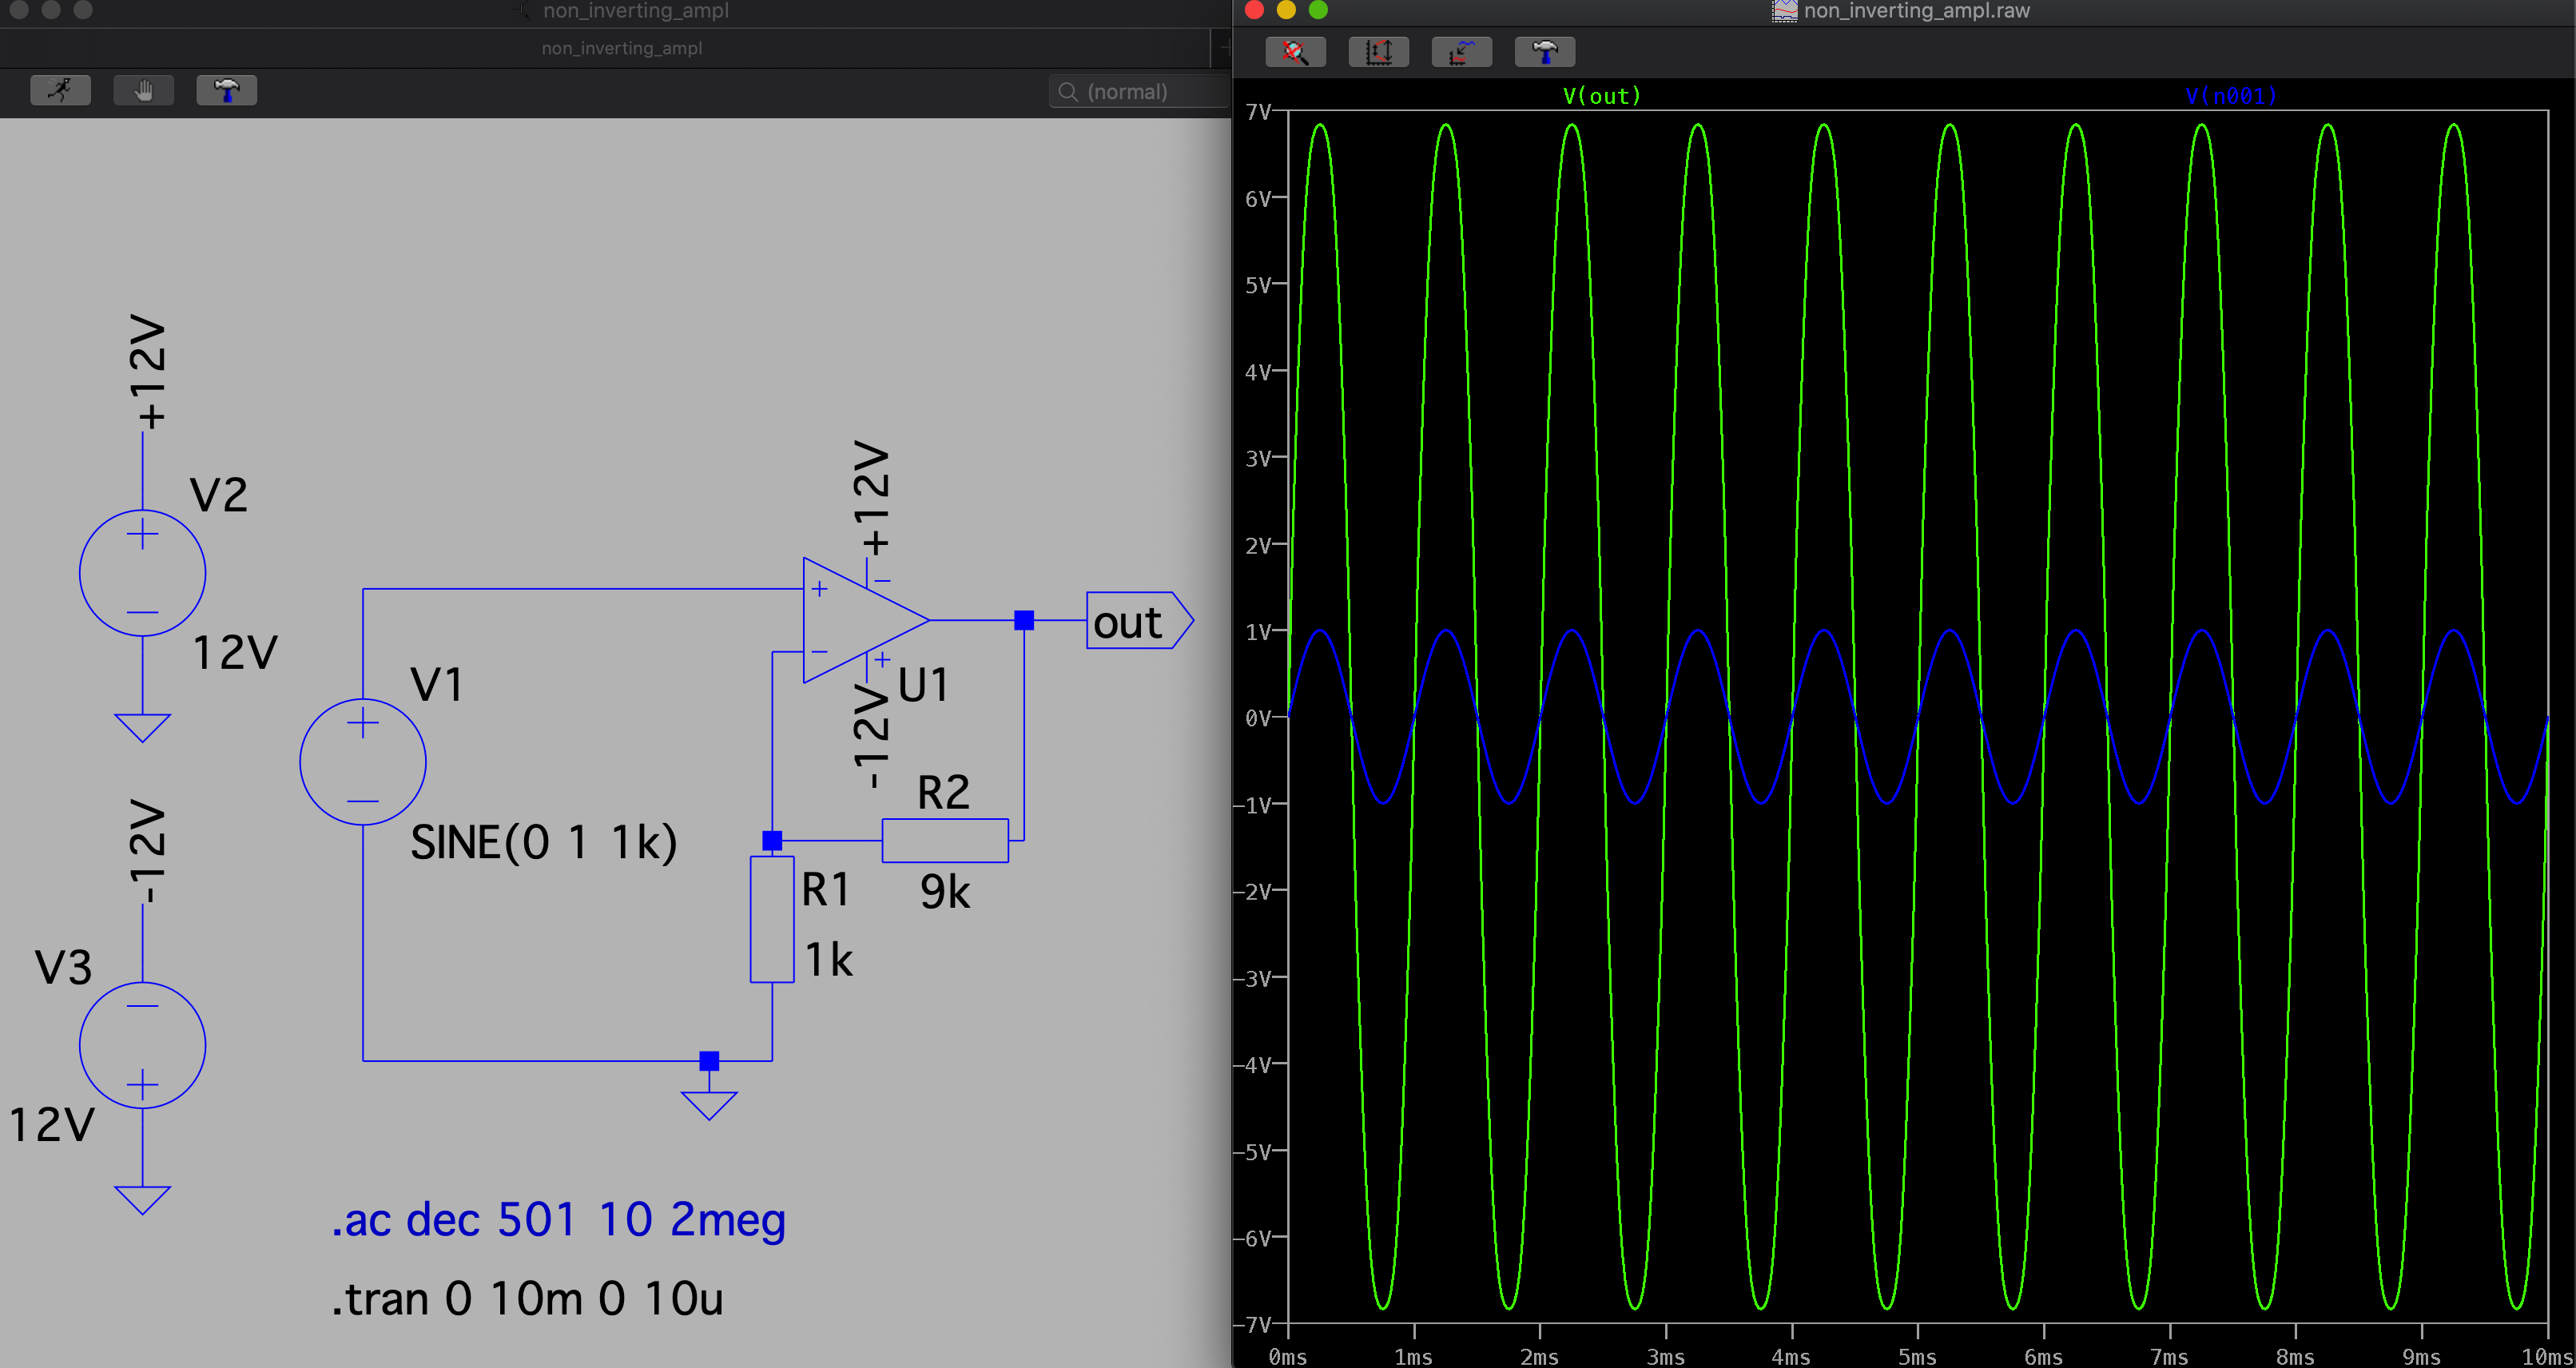
\includegraphics[width=\linewidth]{pictures/analysis_7.png}
                  \end{minipage} 
                  \\
                \end{tabular}
      
              \end{table}
               
              \end{tiny} \end{spacing}

          \end{frame}

          \begin{frame}[t]{OPV Schaltungen - Lösung Grenzfrequenz} 
    
              \begin{spacing}{0.9} \begin{tiny}
                \begin{table}[h!]
                \begin{tabular}{p{10cm}}
                  \hline
                  \textbf{Simulation und Analyse} \\
                  \hline \\
                  \begin{minipage}{\textwidth}
                    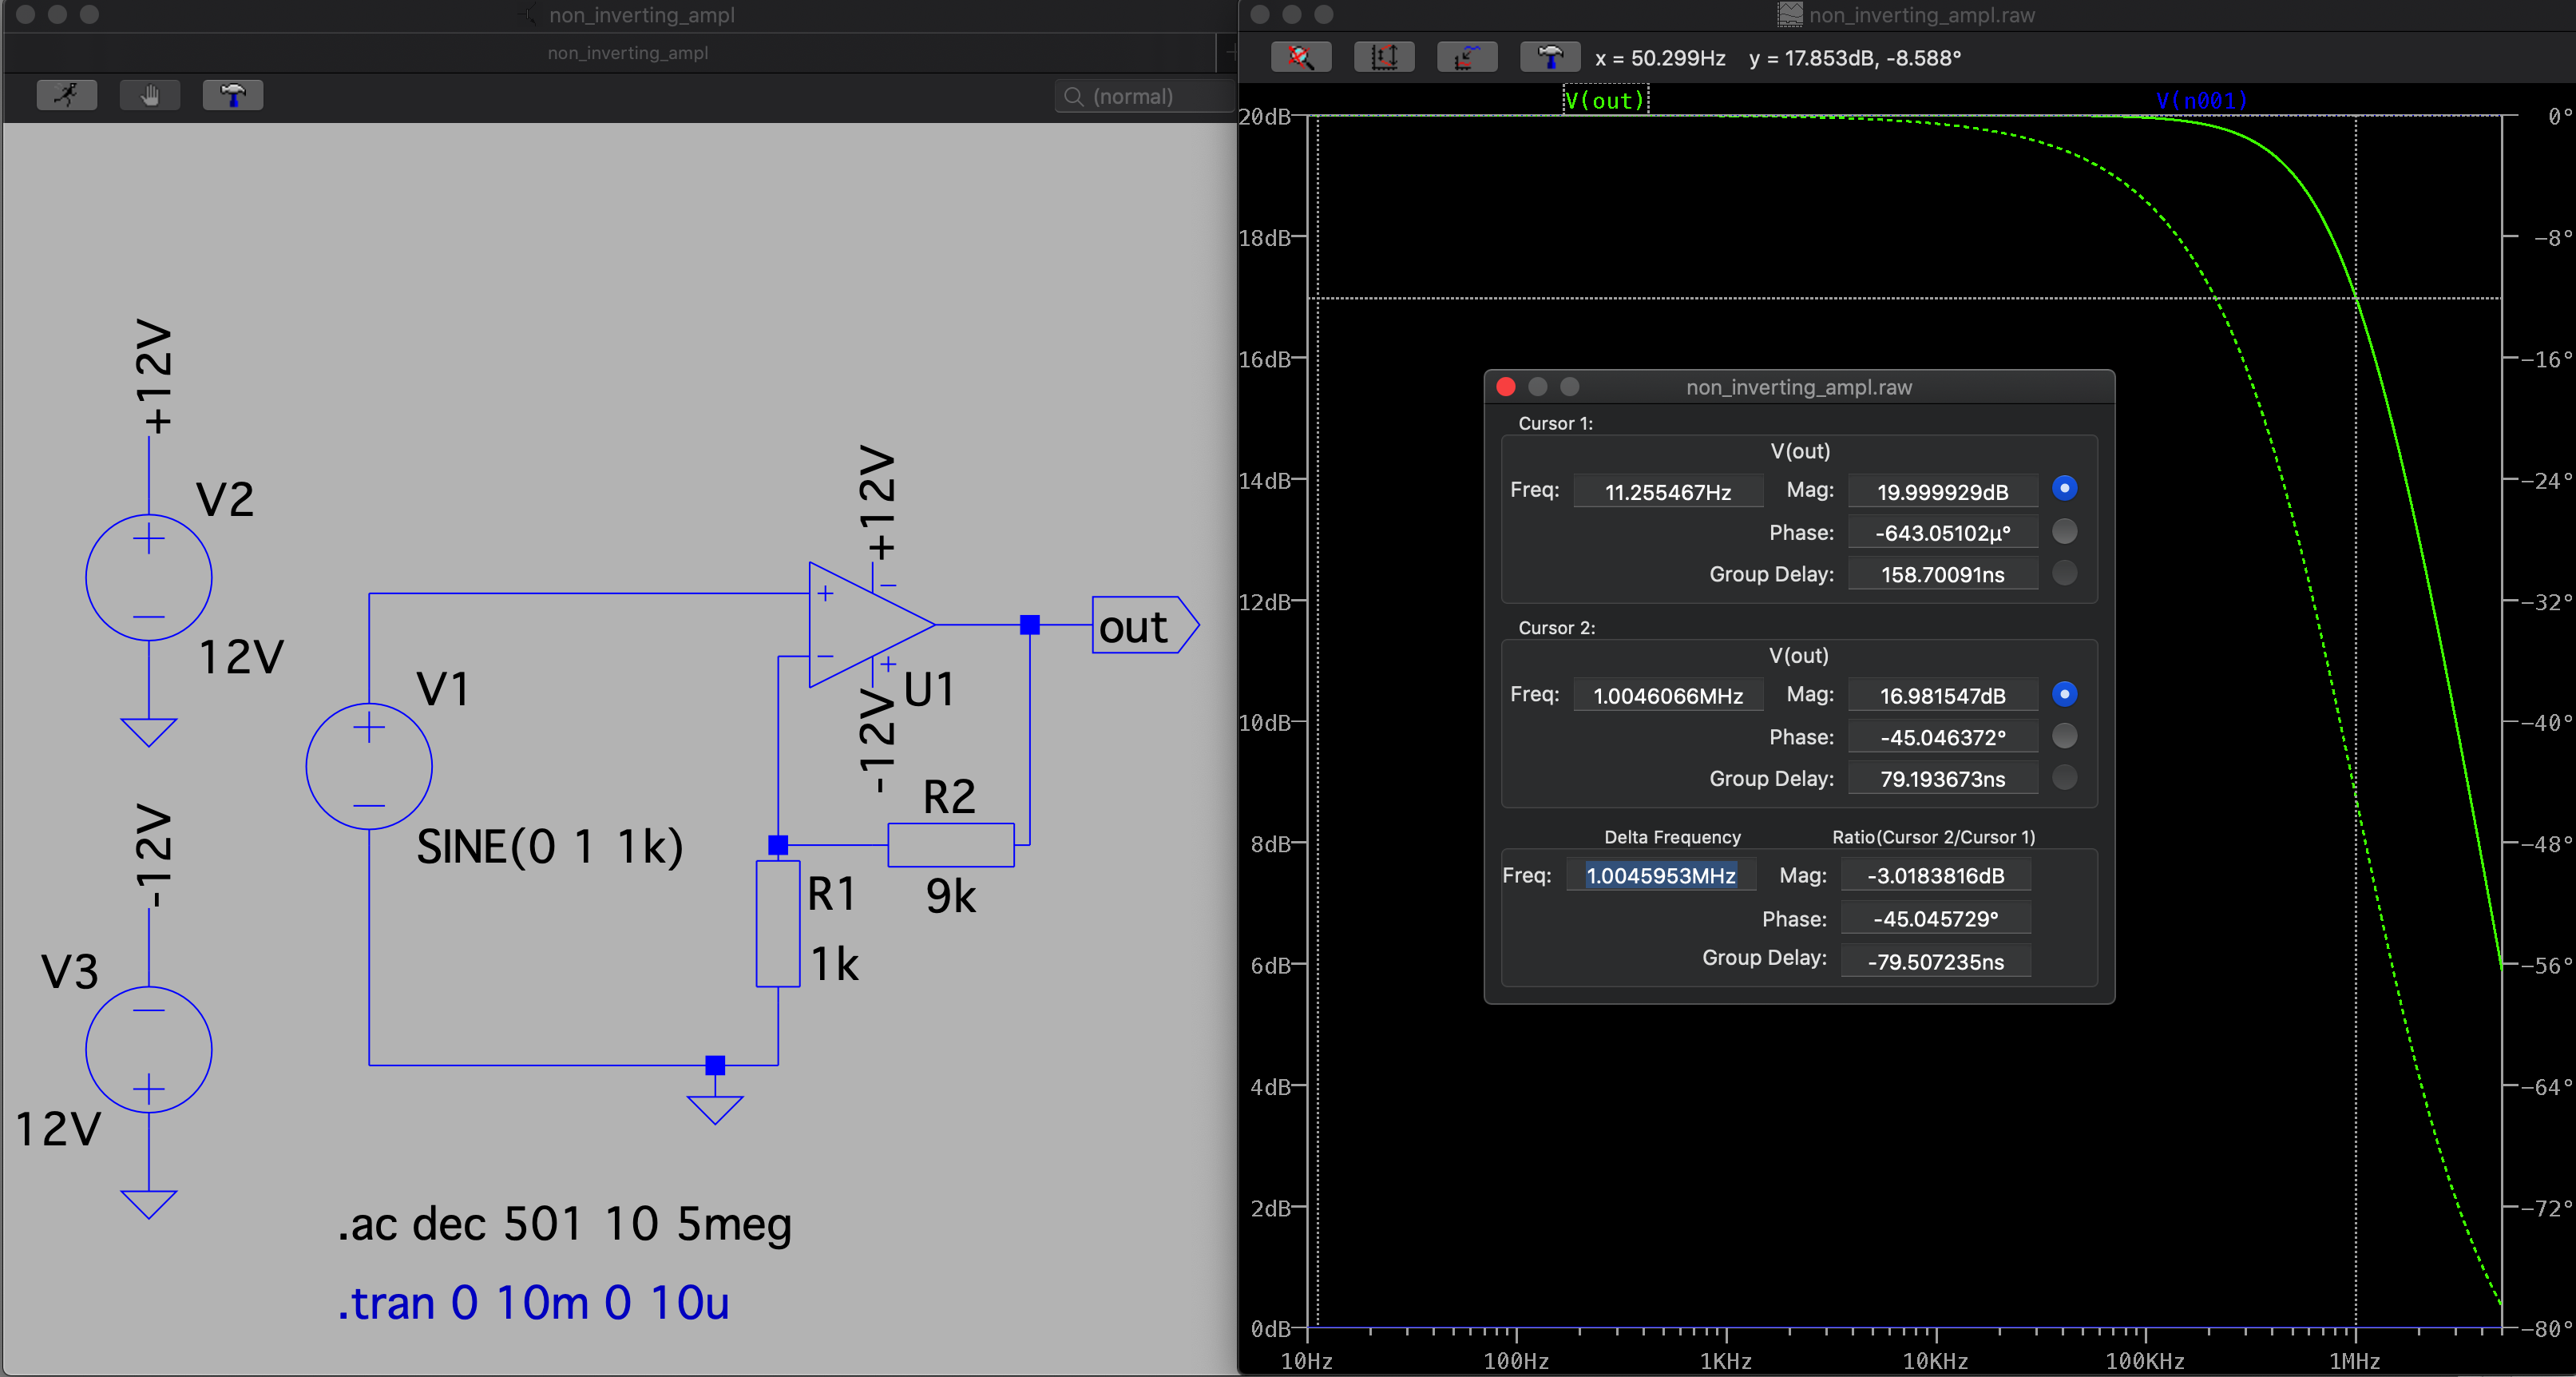
\includegraphics[width=\linewidth]{pictures/bode_2.png}
                  \end{minipage} 
                  \\
                \end{tabular}
      
              \end{table}
               
              \end{tiny} \end{spacing}

          \end{frame}%opv-transient, ac, non inverting
  
\section{Projekt - Temperaturmessbrücke}

\begin{frame}[t]{Überblick}

    \begin{spacing}{0.9} \begin{tiny}
            \begin{minipage}{\textwidth}
                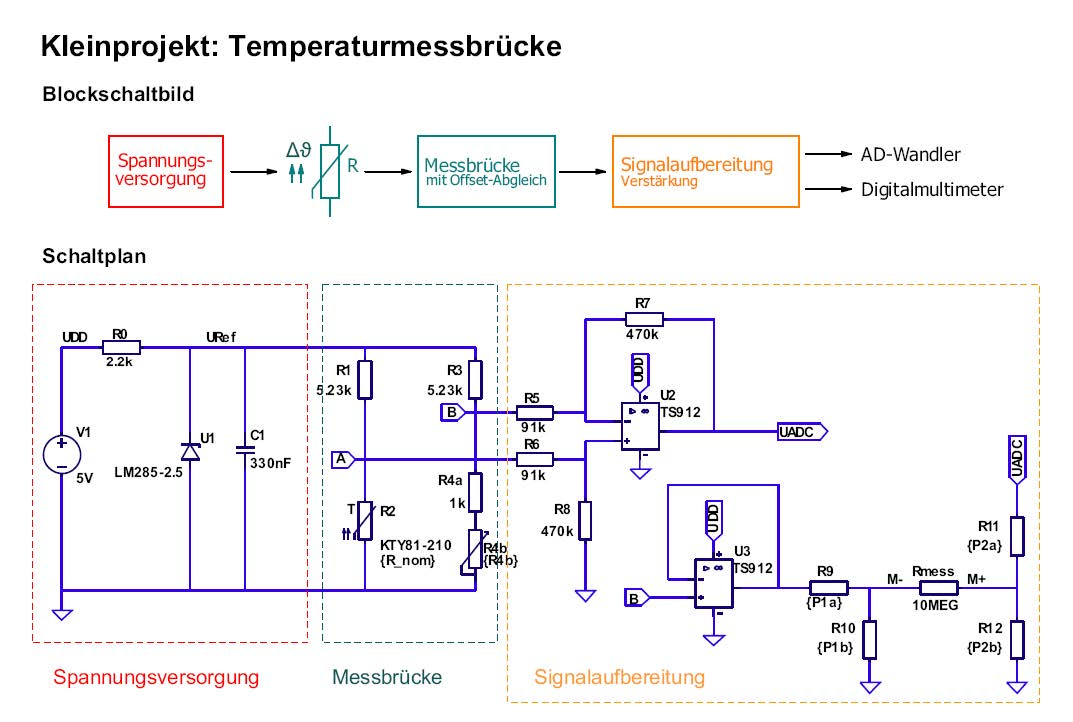
\includegraphics[width=\linewidth]{pictures/projekt_overview.jpg}
            \end{minipage}
        \end{tiny} \end{spacing}

\end{frame}

\begin{frame}[t]{Vorgehenhensweise}

    Zu diesem Zeitpunkt sollten wir alle in der Lage sein einfache Simulationen in DC-,AC-Sweep sowie transient
    durchführen zu können. Sie sollten den Bauteileditor sowie die grundlegenden Schematic-Funktionen (Rotate, Cut, \dots)
    sicher beherrschen.

    Wir werden nun die Bruecke und dir vorgestellten Bestandteile Stück für Stück aufbauen.
    \textbf{Bitte beachtet Folgendes:}

    \begin{enumerate}
        \item Bitte speichert alle Zwischenschritte ab, wir werden Teile später wiederverwenden
        \item Bei Fragen bitten wir euch uns direkt im MS Teams zu benachrichtigen, sodass wir euren
              Fortschritt so gut wie möglich unterstützen können.
    \end{enumerate}
\end{frame}
 % einleitung ins projekt
%\input{messbruecke/brueckenschaltung_op.tex} % Brückenschaltung und OP analyse
%\input{messbruecke/brueckenschaltung_rt.tex} % Brückenschaltung mit variablen Wiederstand
%\input{messbruecke/kty_81.tex} % einführung Kty
%\input{messbruecke/brueckenschaltung_linearisiert.tex} % linearisierung
%\input{messbruecke/brueckenschaltung_diff_amp.tex} % differenzenverstärker
%\input{messbruecke/brueckenschaltung_multimeer.tex} % anpassung multineter
%\input{messbruecke/brueckenschaltung_gesamt.tex} % anpassung multineter


\end{document} 	